\pdfminorversion=4 % for acroread
%\documentclass[aspectratio=169,t,xcolor={usenames,dvipsnames}]{beamer}
\documentclass[aspectratio=169,t,handout,xcolor={usenames,dvipsnames}]{beamer}
\usepackage{../beamerstyle}
\usepackage{dsfont}
\usepackage{bm}
\usepackage[english]{babel}
\usepackage[utf8]{inputenc}
\usepackage{graphicx}
\usepackage{algorithm}
\usepackage[ruled,vlined,algo2e,linesnumbered]{algorithm2e}
%\usepackage[boxed,vlined]{algorithm2e}
\usepackage{hyperref}
\usepackage{booktabs}
\usepackage{mathtools}

\usepackage{amsmath,amssymb}
\usepackage{listings}
\lstset{frame=lines,framesep=3pt,numbers=left,numberblanklines=false,basicstyle=\ttfamily\small}

\usepackage{subfig}
\usepackage{multicol}
%\usepackage{appendixnumberbeamer}
%
\usepackage{tcolorbox}

\usepackage{pgfplots}
\usepackage{tikz}
\usetikzlibrary{trees} 
\usetikzlibrary{shapes.geometric}
\usetikzlibrary{positioning,shapes,shadows,arrows,calc,mindmap}
\usetikzlibrary{positioning,fadings,through}
\usetikzlibrary{decorations.pathreplacing}
\usetikzlibrary{intersections}
\usetikzlibrary{positioning,fit,calc,shadows,backgrounds}
\pgfdeclarelayer{background}
\pgfdeclarelayer{foreground}
\pgfsetlayers{background,main,foreground}
\tikzstyle{activity}=[rectangle, draw=black, rounded corners, text centered, text width=8em]
\tikzstyle{data}=[rectangle, draw=black, text centered, text width=8em]
\tikzstyle{myarrow}=[->, thick, draw=black]

% Define the layers to draw the diagram
\pgfdeclarelayer{background}
\pgfdeclarelayer{foreground}
\pgfsetlayers{background,main,foreground}

%\usepackage{listings}
%\lstset{numbers=left,
%  showstringspaces=false,
%  frame={tb},
%  captionpos=b,
%  lineskip=0pt,
%  basicstyle=\ttfamily,
%%  extendedchars=true,
%  stepnumber=1,
%  numberstyle=\small,
%  xleftmargin=1em,
%  breaklines
%}

 
\definecolor{blue}{RGB}{0, 74, 153}

\usetheme{Boadilla}
%\useinnertheme{rectangles}
\usecolortheme{whale}
\setbeamercolor{alerted text}{fg=blue}
\useoutertheme{infolines}
\setbeamertemplate{navigation symbols}{\vspace{-5pt}} % to lower the logo
\setbeamercolor{date in head/foot}{bg=white} % blue
\setbeamercolor{date in head/foot}{fg=white}
\setbeamercolor{author  in head/foot}{bg=white} %blue
\setbeamercolor{title in head/foot}{bg=white} % blue
\setbeamercolor{title}{fg=white, bg=blue}
\setbeamercolor{block title}{fg=white,bg=blue}
\setbeamercolor{block body}{bg=blue!10}
\setbeamercolor{frametitle}{fg=white, bg=blue}
\setbeamercovered{invisible}

\makeatletter
\setbeamertemplate{footline}
{
  \leavevmode%
  \hbox{%
  \begin{beamercolorbox}[wd=.333333\paperwidth,ht=2.25ex,dp=1ex,center]{author in head/foot}%
%    \usebeamerfont{author in head/foot}\insertshortauthor
  \end{beamercolorbox}%
  \begin{beamercolorbox}[wd=.333333\paperwidth,ht=2.25ex,dp=1ex,center]{title in head/foot}%
    \usebeamerfont{title in head/foot}\insertshorttitle
  \end{beamercolorbox}%
  \begin{beamercolorbox}[wd=.333333\paperwidth,ht=2.25ex,dp=1ex,right]{date in head/foot}%
    \usebeamerfont{date in head/foot}\insertshortdate{}\hspace*{2em}
%    \insertframenumber\hspace*{2ex} 
  \end{beamercolorbox}}%
  \vskip0pt%
}
\makeatother

%\pgfdeclareimage[height=1.2cm]{automl}{images/logos/automl.png}
%\pgfdeclareimage[height=1.2cm]{freiburg}{images/logos/freiburg}

%\logo{\pgfuseimage{freiburg}}

\renewcommand{\comment}[1]{
	\noindent
	%\vspace{0.25cm}
	{\color{red}{\textbf{TODO:} #1}}
	%\vspace{0.25cm}
}
\newcommand{\notefh}[1]{\textcolor{red}{\textbf{FH:} #1}}
\renewcommand{\comment}[1]{}
\newcommand{\hide}[1]{}
\newcommand{\cemph}[2]{\emph{\textcolor{#1}{#2}}}

\newcommand{\lit}[1]{{\footnotesize\color{black!60}[#1]}}

\newcommand{\litw}[1]{{\footnotesize\color{blue!20}[#1]}}


\newcommand{\myframe}[2]{\begin{frame}[c]{#1}#2\end{frame}}
\newcommand{\myframetop}[2]{\begin{frame}{#1}#2\end{frame}}
\newcommand{\myit}[1]{\begin{itemize}#1\end{itemize}}
\newcommand{\myblock}[2]{\begin{block}{#1}#2\end{block}}


\newcommand{\votepurple}[1]{\textcolor{Purple}{$\bigstar$}}
\newcommand{\voteyellow}[1]{\textcolor{Goldenrod}{$\bigstar$}}
\newcommand{\voteblue}[1]{\textcolor{RoyalBlue}{$\bigstar$}}
\newcommand{\votepink}[1]{\textcolor{Pink}{$\bigstar$}}

\newcommand{\diff}{\mathop{}\!\mathrm{d}}
\newcommand{\refstyle}[1]{{\small{\textcolor{gray}{#1}}}}
\newcommand{\hands}[0]{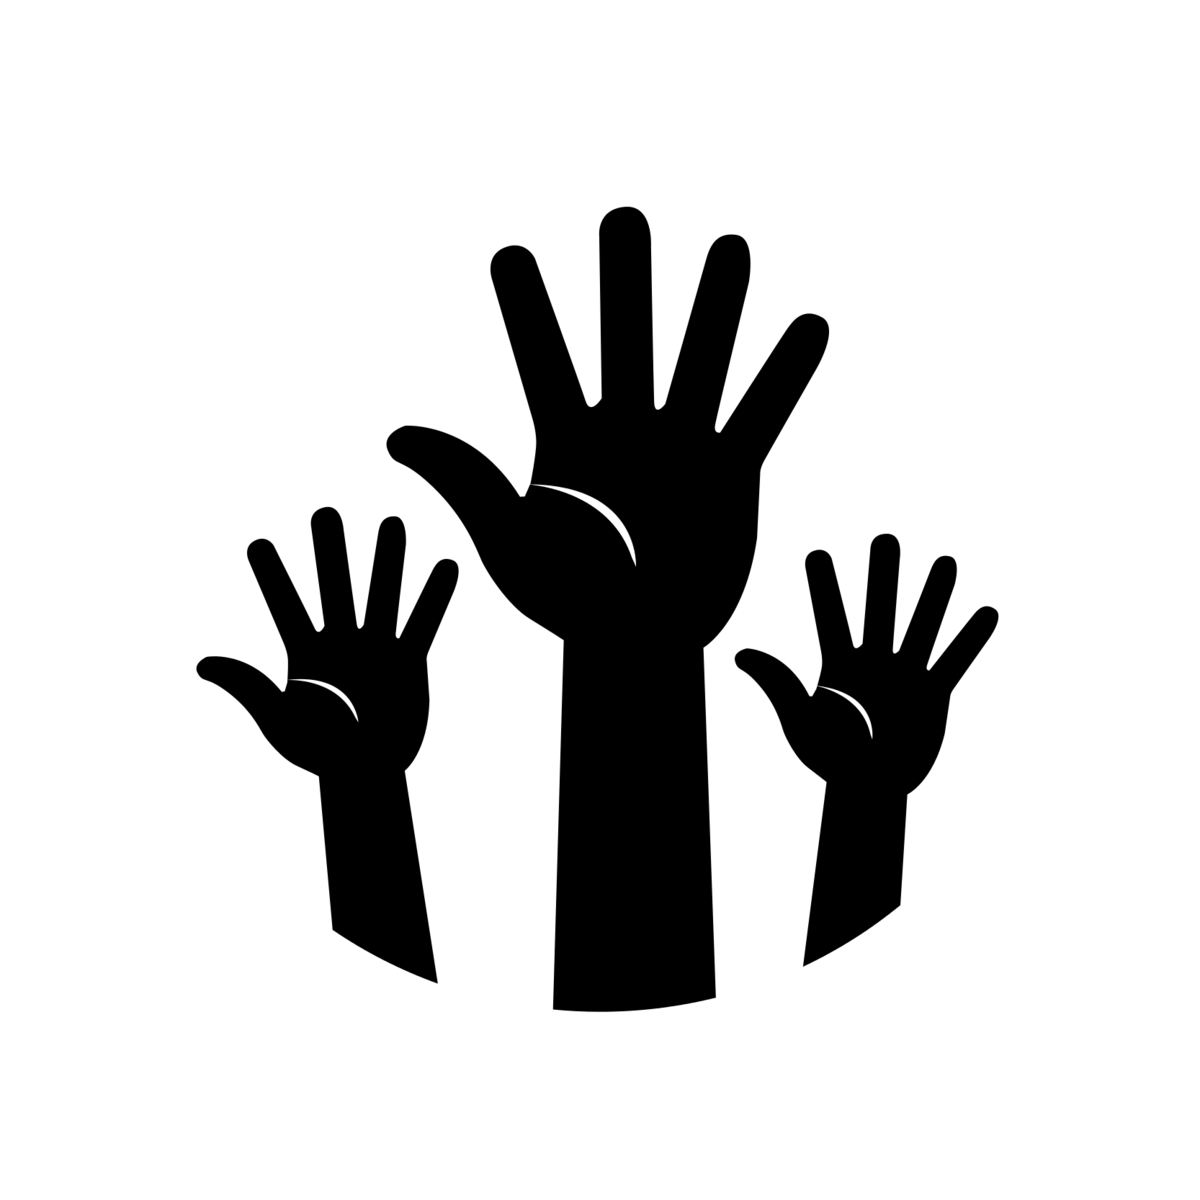
\includegraphics[height=1.5em]{images/hands}}
\newcommand{\transpose}[0]{{\textrm{\tiny{\sf{T}}}}}
\newcommand{\norm}{{\mathcal{N}}}
\newcommand{\cutoff}[0]{\kappa}
\newcommand{\instD}[0]{\dataset}
\newcommand{\insts}[0]{\mathcal{I}}
\newcommand{\inst}[0]{i}
\newcommand{\instI}[1]{i^{(#1)}}

% Iteration specific instance of variable/function/anything
% Introduced in the BO section, but moved up here to make it available within other macros
\newcommand{\iter}[2][\bocount]{{#2}^{(#1)}}

%--------HPO parameter macros-----------

% Parameter Configuration Space
\newcommand{\pcs}[0]{\pmb{\Lambda}}

% ???
\newcommand{\bx}[0]{\conf}

% Parameter Configuration
\newcommand{\conf}[0]{\pmb{\lambda}}

% Final Configuration
\newcommand{\finconf}[0]{\pmb{\hat{\lambda}}}

% Configuration corresponding to a given iteration -- better use \iter!
\newcommand{\confI}[1]{{\conf}^{(#1)}}

% Default Configuration
\newcommand{\defconf}[0]{{\conf}_{\text{def}}}

% Incumbent Configuration
\newcommand{\incumbent}[1][\bocount]{\iter[#1]{\finconf}}

% Optimal Configuration
\newcommand{\optconf}[0]{{\conf}^*}

% Configuration Space
\newcommand{\confs}[0]{\pcs}

%----------------------------------------

%\newcommand{\vlambda}[0]{\bm{\lambda}}
%\newcommand{\vLambda}[0]{\bm{\Lambda}}
\newcommand{\dataset}[0]{\mathcal{D}}
\newcommand{\datasets}[0]{\mathbf{D}}
\newcommand{\loss}[0]{L}
\newcommand{\risk}{\mathcal{R}}
\newcommand{\riske}{\mathcal{R}_{\text{emp}}}
\newcommand{\cost}[0]{c}
\newcommand{\costI}[1]{c^{(#1)}}

% Gaussian Process
\newcommand{\gp}{\mathcal{G}}
% Family of Objective Functions
\newcommand{\objF}{F}

%---------------BO Macros------------------

% BO loop counter
\newcommand{\bocount}{t}
% BO loop counter max, the counter runs from 1 to this value
\newcommand{\bobudget}{T}
% BO loop observation
\newcommand{\obs}[1][\conf]{\cost({#1})}
% BO loop observation space
\newcommand{\obsspace}{\mathcal{Y}}
% BO loop next observation
\newcommand{\bonextobs}{\obs[\iter{\conf}]}
% Acquisition Function, no args
\newcommand{\acq}{u}
% Standard Normal PDF
\newcommand{\pdf}{\phi}
% Standard Normal CDF
\newcommand{\cdf}{\Phi}
% Mean
\newcommand{\mean}{\mu}
% Standard Deviation
\newcommand{\stddev}{\sigma}
% Variance
\newcommand{\variance}{\sigma^2}
% Noise
\newcommand{\noise}{\nu}
% BO loop next selected sample
\newcommand{\bonextsample}{\confI{\bocount}}

% Single hyperparameter
\newcommand{\hyperparam}{\lambda}

% Single hyperparameter within a hyperparameter configuration
\newcommand{\hyperparami}[1][i]{{\hyperparam}_#1}

% Full definition of final configuration
\newcommand{\finconffull}{\incumbent[\bobudget]}

% Dataset
\newcommand{\datasetHPO}{{\dataset}_{HPO}}

% Dataset definition
\newcommand{\datasetHPOdef}{{\langle \bonextsample,\,\bonextobs \rangle}_{\bocount=1}^{\bobudget}}

% Double Display Fraction, forces large displays for everything in numerator and denominator
\newcommand\ddfrac[2]{\frac{\displaystyle #1}{\displaystyle #2}}

% Conditional Probability "Given That" Relation, source:https://tex.stackexchange.com/a/141685/205886
\newcommand\given[1][]{\:#1\vert\:}

% Expectation as a math operator
\DeclareMathOperator*{\E}{\mathbb{E}}

% Citation 
\newcommand{\source}[1]{
    \begin{flushright}
    	Source: \lit{#1}
    \end{flushright}
}
%-------------------------------------------

%Real numbers set
\newcommand{\realnum}{\mathbb{R}}
%Configuration space - do not use
%\newcommand{\configspace}{\Theta}
%Instances - do not use
%\newcommand{\instances}{\mathcal{I}}
%Expected value
\newcommand{\expectation}{\mathbb{E}}
%Kernel
\newcommand{\kernel}{\kappa}
%Constraint function
\newcommand{\constraintf}{c}
%Normal distribution
\newcommand{\normaldist}{\mathcal{N}}

% \renewcommand{\vec}[1]{\mathbf{#1}}
\newcommand{\hist}[0]{\dataset_{\text{Hist}}}
\newcommand{\param}[0]{p}
\newcommand{\algo}[0]{\mathcal{A}}
\newcommand{\algos}[0]{\mathbf{A}}
%\newcommand{\nn}[0]{N}
\newcommand{\feats}[0]{\mathcal{X}_{\text{meta}}}
\newcommand{\feat}[0]{\x_{\text{meta}}}
%\newcommand{\cluster}[0]{\vec{h}}
%\newcommand{\clusters}[0]{\vec{H}}
\newcommand{\perf}[0]{\mathbb{R}}
%\newcommand{\surro}[0]{\mathcal{S}}
\newcommand{\surro}[0]{\hat{\cost}}
\newcommand{\func}[0]{f}
\newcommand{\epm}[0]{\surro}
\newcommand{\portfolio}[0]{\mathbf{P}}
\newcommand{\schedule}[0]{\mathcal{S}}

% Machine Learning
\newcommand{\mdata}[0]{\dataset_{\text{meta}}}
\newcommand{\datasettrain}[0]{\dataset_{\text{train}}}
\newcommand{\datasetval}[0]{\dataset_{\text{val}}}
\newcommand{\datasettest}[0]{\dataset_{\text{test}}}
\newcommand{\x}[0]{\mathbf{x}}
\newcommand{\y}[0]{y}
\newcommand{\xI}[1]{\mathbf{x}^{(#1)}}
\newcommand{\yI}[1]{y^{(#1)}}
\newcommand{\fx}{f(\mathbf{x})}  % f(x), continuous prediction function
\newcommand{\Hspace}{\mathcal{H}} % hypothesis space where f is from
\newcommand{\fh}{\hat{f}}       % f hat, estimated prediction function

% Deep Learning
\newcommand{\weights}[0]{\theta}
\newcommand{\metaweights}[0]{\phi}


% reinforcement learning
\newcommand{\policies}[0]{\mathbf{\Pi}}
\newcommand{\policy}[0]{\pi}
\newcommand{\actionRL}[0]{a}
\newcommand{\stateRL}[0]{s}
\newcommand{\statesRL}[0]{\mathcal{S}}
\newcommand{\rewardRL}[0]{r}
\newcommand{\rewardfuncRL}[0]{\mathcal{R}}

\RestyleAlgo{algoruled}
\DontPrintSemicolon
\LinesNumbered
\SetAlgoVlined
\SetFuncSty{textsc}

\SetKwInOut{Input}{Input}
\SetKwInOut{Output}{Output}
\SetKw{Return}{return}

%\newcommand{\changed}[1]{{\color{red}#1}}

%\newcommand{\citeN}[1]{\citeauthor{#1}~(\citeyear{#1})}

\renewcommand{\vec}[1]{\mathbf{#1}}
\DeclareMathOperator*{\argmin}{arg\,min}
\DeclareMathOperator*{\argmax}{arg\,max}

%\newcommand{\aqme}{\textit{AQME}}
%\newcommand{\aslib}{\textit{ASlib}}
%\newcommand{\llama}{\textit{LLAMA}}
%\newcommand{\satzilla}{\textit{SATzilla}}
%\newcommand{\satzillaY}[1]{\textit{SATzilla'{#1}}}
%\newcommand{\snnap}{\textit{SNNAP}}
%\newcommand{\claspfolioTwo}{\textit{claspfolio~2}}
%\newcommand{\flexfolio}{\textit{FlexFolio}}
%\newcommand{\claspfolioOne}{\textit{claspfolio~1}}
%\newcommand{\isac}{\textit{ISAC}}
%\newcommand{\eisac}{\textit{EISAC}}
%\newcommand{\sss}{\textit{3S}}
%\newcommand{\sunny}{\textit{Sunny}}
%\newcommand{\ssspar}{\textit{3Spar}}
%\newcommand{\cshc}{\textit{CSHC}}
%\newcommand{\cshcpar}{\textit{CSHCpar}}
%\newcommand{\measp}{\textit{ME-ASP}}
%\newcommand{\aspeed}{\textit{aspeed}}
%\newcommand{\autofolio}{\textit{AutoFolio}}
%\newcommand{\cedalion}{\textit{Cedalion}}
\newcommand{\fanova}{\textit{fANOVA}}
\newcommand{\sbs}{\textit{SB}}
\newcommand{\oracle}{\textit{VBS}}

% like approaches
\newcommand{\claspfoliolike}[1]{\texttt{claspfolio-#1-like}}
\newcommand{\satzillalike}[1]{\texttt{SATzilla'#1-like}}
\newcommand{\isaclike}{\texttt{ISAC-like}}
\newcommand{\ssslike}{\texttt{3S-like}}
\newcommand{\measplike}{\texttt{ME-ASP-like}}

\newcommand{\irace}{\textit{I/F-race}}
\newcommand{\gga}{\textit{GGA}}
\newcommand{\smac}{\textit{SMAC}}
\newcommand{\paramils}{\textit{ParamILS}}
\newcommand{\spearmint}{\textit{Spearmint}}
\newcommand{\tpe}{\textit{TPE}}


\usepackage{pifont}
\newcommand{\itarrow}{\mbox{\Pisymbol{pzd}{229}}}
\newcommand{\ithook}{\mbox{\Pisymbol{pzd}{52}}}
\newcommand{\itcross}{\mbox{\Pisymbol{pzd}{56}}}
\newcommand{\ithand}{\mbox{\raisebox{-1pt}{\Pisymbol{pzd}{43}}}}

%\DeclareMathOperator*{\argmax}{arg\,max}

\newcommand{\ie}{{\it{}i.e.\/}}
\newcommand{\eg}{{\it{}e.g.\/}}
\newcommand{\cf}{{\it{}cf.\/}}
\newcommand{\wrt}{\mbox{w.r.t.}}
\newcommand{\vs}{{\it{}vs\/}}
\newcommand{\vsp}{{\it{}vs\/}}
\newcommand{\etc}{{\copyedit{etc.}}}
\newcommand{\etal}{{\it{}et al.\/}}

\newcommand{\pscProc}{{\bf procedure}}
\newcommand{\pscBegin}{{\bf begin}}
\newcommand{\pscEnd}{{\bf end}}
\newcommand{\pscEndIf}{{\bf endif}}
\newcommand{\pscFor}{{\bf for}}
\newcommand{\pscEach}{{\bf each}}
\newcommand{\pscThen}{{\bf then}}
\newcommand{\pscElse}{{\bf else}}
\newcommand{\pscWhile}{{\bf while}}
\newcommand{\pscIf}{{\bf if}}
\newcommand{\pscRepeat}{{\bf repeat}}
\newcommand{\pscUntil}{{\bf until}}
\newcommand{\pscWithProb}{{\bf with probability}}
\newcommand{\pscOtherwise}{{\bf otherwise}}
\newcommand{\pscDo}{{\bf do}}
\newcommand{\pscTo}{{\bf to}}
\newcommand{\pscOr}{{\bf or}}
\newcommand{\pscAnd}{{\bf and}}
\newcommand{\pscNot}{{\bf not}}
\newcommand{\pscFalse}{{\bf false}}
\newcommand{\pscEachElOf}{{\bf each element of}}
\newcommand{\pscReturn}{{\bf return}}

%\newcommand{\param}[1]{{\sl{}#1}}
\newcommand{\var}[1]{{\it{}#1}}
\newcommand{\cond}[1]{{\sf{}#1}}
%\newcommand{\state}[1]{{\sf{}#1}}
%\newcommand{\func}[1]{{\sl{}#1}}
\newcommand{\set}[1]{{\Bbb #1}}
%\newcommand{\inst}[1]{{\tt{}#1}}
\newcommand{\myurl}[1]{{\small\sf #1}}

\newcommand{\Nats}{{\Bbb N}}
\newcommand{\Reals}{{\Bbb R}}
\newcommand{\extset}[2]{\{#1 \; | \; #2\}}

\newcommand{\vbar}{$\,\;|$\hspace*{-1em}\raisebox{-0.3mm}{$\,\;\;|$}}
\newcommand{\vendbar}{\raisebox{+0.4mm}{$\,\;|$}}
\newcommand{\vend}{$\,\:\lfloor$}


\newcommand{\goleft}[2][.7]{\parbox[t]{#1\linewidth}{\strut\raggedright #2\strut}}
\newcommand{\rightimage}[2][.3]{\mbox{}\hfill\raisebox{1em-\height}[0pt][0pt]{\includegraphics[width=#1\linewidth]{#2}}\vspace*{-\baselineskip}}





% Bayesian Optimization SS 2020 macros
\def\Put(#1,#2)#3{\leavevmode\makebox(0,0){\put(#1,#2){#3}}}

% FH: I created this command videotitle (and file title_slide.tex) to show a new title slide for each video without the need of any repeating boiler plate code. Please do not change this anymore.
\newcommand{\videotitle}[1]{\subtitle{#1}%%%%%%%%%%%%%%%%% Title slide -- only change title %%%%%%%%%%%%%%%
%\title{\lecturetitle}
%\subtitle{\weektitle}
%\\\vspace*{0.3cm}
% ---------------------------------------------------------------------
{
\setbeamertemplate{footline}{} % remove footer on first slide
	\frame[c]{
	\titlepage
	}
}
}
\newcommand{\fhpause}{\pause} % for taping

% for final handout:
\renewcommand{\videotitle}[1]{\subtitle{#1}\section{#1}%%%%%%%%%%%%%%%%% Title slide -- only change title %%%%%%%%%%%%%%%
%\title{\lecturetitle}
%\subtitle{\weektitle}
%\\\vspace*{0.3cm}
% ---------------------------------------------------------------------
{
\setbeamertemplate{footline}{} % remove footer on first slide
	\frame[c]{
	\titlepage
	}
}
}
\renewcommand{\fhpause}{} % for final handout

\title[Speedup Techniques for Hyperparameter Optimization]{Speedup Techniques for Hyperparameter Optimization} % week title
\author[Frank Hutter]{Bernd Bischl \and \underline{Frank Hutter} \and Lars Kotthoff\newline \and Marius Lindauer \and Joaquin Vanschoren}
\institute{}
\date{}


\AtBeginSection[] % Show a table of contents between videos for easier navigation and making available a single PDF per lecture. 
{
  \begin{frame}{Outline}
    \bigskip
    \vfill
    \tableofcontents[currentsection]
  \end{frame}
}


\begin{document}
	
\maketitle
%%-------------------------------------------------
\begin{frame}{Beyond Black-box Optimization}
\medskip
Recall general blackbox optimization:\\
        \bigskip
        \begin{center}
        \scalebox{0.7}{\hspace*{1.0cm}
        \newcommand{\myblackbox}{\fcolorbox{black}{black}{
    \minipage[t]{\dimexpr0.111\linewidth-2\fboxsep-2\fboxrule\relax}
        ~~~\\
        ~~~\\
        ~~~\\
    \endminipage}}
    
    
    	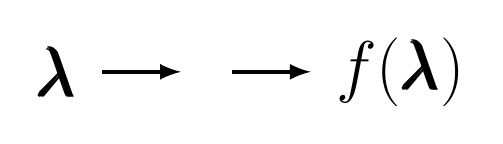
\begin{tikzpicture}
\tikzstyle{every node}=[draw,fill=white,minimum width=0cm,thin]
\tikzstyle{every path}=[-latex,ultra thick]
\node (A) [draw=white]{{\Huge{$\conf$}}};
\node (B) [right=14mm of A,draw=white] {\myblackbox{}};
\node (C) [right=14mm of B,draw=white] {{\Huge{$f(\conf)$}}};
%\node (D) [below=7mm of B, align=center, fill=black!10] {\large{Bayesian}\\\large{optimization}};

\draw ($(A.east)+(0.2,0.0)$) -- ($(B.west)+(-0.2,0.0)$);
\draw ($(B.east)+(0.2,0.0)$) -- ($(C.west)+(-0.2,0.0)$);
%\draw ($(C.south)+(0.0,-0.2)$) -| ++(0.0,0.0) |- ($(D.east)+(0.2,0.0)$);
%\draw ($(D.west)+(-0.2,0.0)$) |- ++(0.0,0.0) -| ($(A.south)+(0.0,-0.2)$);
\end{tikzpicture}
}\\
        \bigskip
         Only mode of interaction with $f$: querying $f$'s value at a given $\conf$
        
\pause
        \bigskip
        \bigskip
        \huge{\textcolor{red}{Too slow for tuning expensive models}}
        
        \end{center}
\vspace*{-6cm}
\begin{center}
\scalebox{15}{\color{Red}{$\bm{\times}$}}
\end{center}    
    
\end{frame}
%-------------------------------------------------

%-------------------------------------------------
%  \begin{frame}{Outline}
%    \bigskip
%    \vfill
%    \tableofcontents
%  \end{frame}
%-------------------------------------------------

\begin{frame}[c]{Methods for Going Beyond Blackbox Bayesian Optimization}

\begin{columns}

    \column{0.5\textwidth}
    \begin{itemize}
        \item One possible cheap approximation of an expensive function: use a data subset
        \begin{itemize}
            \item Many cheap evaluations on small subsets
            \item Few expensive evaluations on the full data
        \end{itemize}
    \end{itemize}
    
    \column{0.5\textwidth}
    \begin{figure}
        \centering
        \includegraphics[width=0.3\textwidth]{w07_hpo_grey_box/images/intro/black_blocks.png}
    \end{figure}

\end{columns}

\begin{itemize}
    \item E.g.: Support Vector Machines (SVM) on MNIST dataset (hyperparameters: C, $\gamma$)
\end{itemize}

% Screen shots were clipped to 114, 500, 1860, 940
\only<1>{
    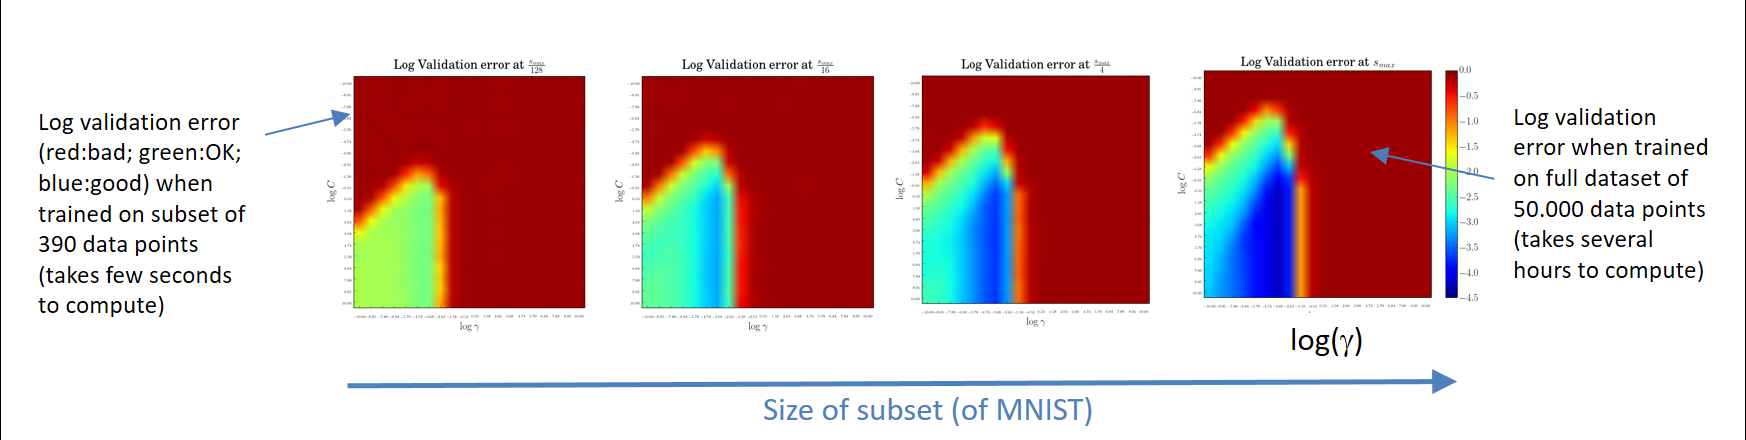
\includegraphics[width=\textwidth,trim=5px 10px 5px 10px, clip]{w07_hpo_grey_box/images/intro/animation_1.png}
}

\only<2->{
    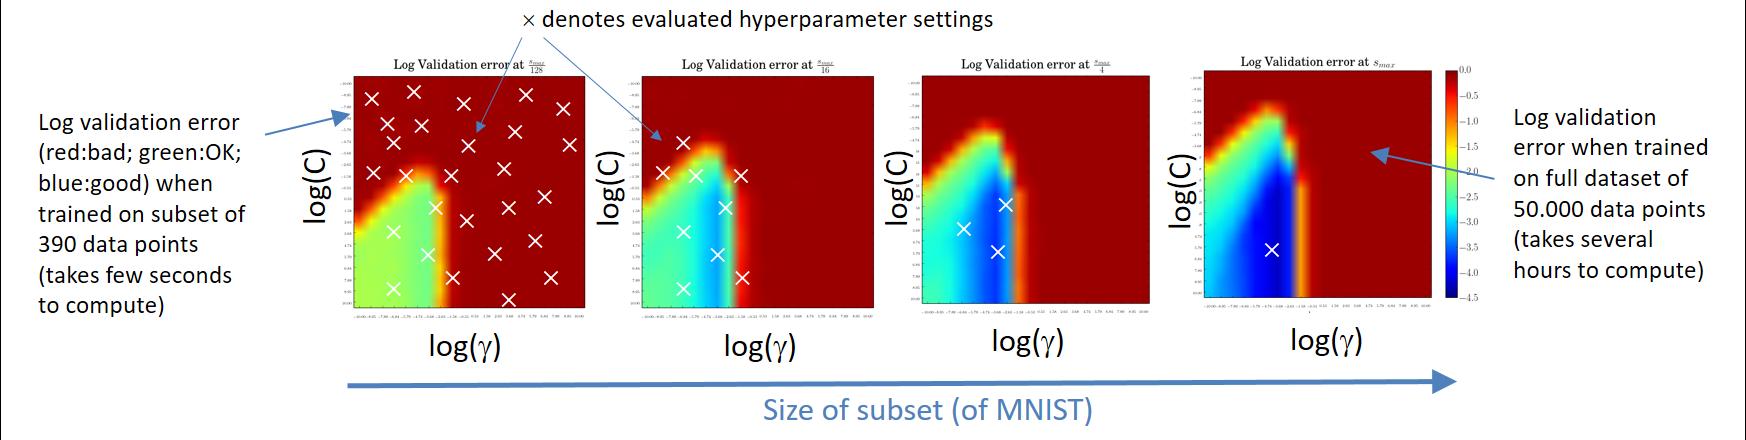
\includegraphics[width=\textwidth,trim=5px 10px 5px 10px, clip]{w07_hpo_grey_box/images/intro/animation_2.png}
}

\vskip -15pt

\only<3->{
    $\rightarrow$ up to 1000x speedups over blackbox optimization on full data \lit{\href{http://proceedings.mlr.press/v54/klein17a/klein17a.pdf}{Klein et al, AISTATS 2017}}
}

\end{frame}

%-----------------------------------------------------------------------

\begin{frame}[c]{Learning Goals of this Lecture}
\framesubtitle{After this lecture, students can ...}

\begin{itemize}
    \item Describe many different ways of using \alert{meta-learning} to speed up HPO
    \item Discuss several ways of predicting \alert{learning curves}
    \item Explain how to \alert{exploit multiple fidelities in Bayesian optimization} 
    \item Explain the \alert{Successive Halving} and \alert{Hyperband} algorithms 
    \item Explain how to combine Bayesian optimization and Hyperband in \alert{BOHB}
    \item Discuss \alert{success stories} of speeding up Bayesian optimization
\end{itemize}
\end{frame}

%-----------------------------------------------------------------------











%-------------------------------------------------
\iffalse


%-------------------------------------------------
\begin{frame}{Recall: Black-box optimization}

\begin{figure}
    \centering
    


\tikzset{every picture/.style={line width=0.75pt}} %set default line width to 0.75pt        

\begin{tikzpicture}[x=0.70pt,y=0.70pt,yscale=-1,xscale=1]
%uncomment if require: \path (0,300); %set diagram left start at 0, and has height of 300

%Straight Lines [id:da5075678478287002] 
\draw    (74.5,104) -- (218.5,104) ;
\draw [shift={(220.5,104)}, rotate = 180] [color={rgb, 255:red, 0; green, 0; blue, 0 }  ][line width=0.75]    (10.93,-3.29) .. controls (6.95,-1.4) and (3.31,-0.3) .. (0,0) .. controls (3.31,0.3) and (6.95,1.4) .. (10.93,3.29)   ;
%Shape: Square [id:dp6368535923226633] 
\draw  [fill={rgb, 255:red, 0; green, 25; blue, 255 }  ,fill opacity=1 ] (14,79) -- (64,79) -- (64,129) -- (14,129) -- cycle ;
%Shape: Square [id:dp8011400143211207] 
\draw  [fill={rgb, 255:red, 0; green, 25; blue, 255 }  ,fill opacity=1 ] (561,79) -- (611,79) -- (611,129) -- (561,129) -- cycle ;
%Straight Lines [id:da6772752516220095] 
\draw    (401.5,101) -- (540.5,101.99) ;
\draw [shift={(542.5,102)}, rotate = 180.41] [color={rgb, 255:red, 0; green, 0; blue, 0 }  ][line width=0.75]    (10.93,-3.29) .. controls (6.95,-1.4) and (3.31,-0.3) .. (0,0) .. controls (3.31,0.3) and (6.95,1.4) .. (10.93,3.29)   ;
%Straight Lines [id:da7102938160527976] 
\draw    (39.5,242) -- (39.01,143) ;
\draw [shift={(39,141)}, rotate = 449.72] [color={rgb, 255:red, 0; green, 0; blue, 0 }  ][line width=0.75]    (10.93,-3.29) .. controls (6.95,-1.4) and (3.31,-0.3) .. (0,0) .. controls (3.31,0.3) and (6.95,1.4) .. (10.93,3.29)   ;
%Straight Lines [id:da5275375794470956] 
\draw    (39.5,242) -- (123.5,242) ;
%Straight Lines [id:da11206880859629287] 
\draw    (123.5,242) -- (586.5,242) ;
%Straight Lines [id:da8957848321230528] 
\draw    (586.5,135) -- (586.5,242) ;
%Image [id:dp5678753924043267] 
\draw (313.5,101.5) node  {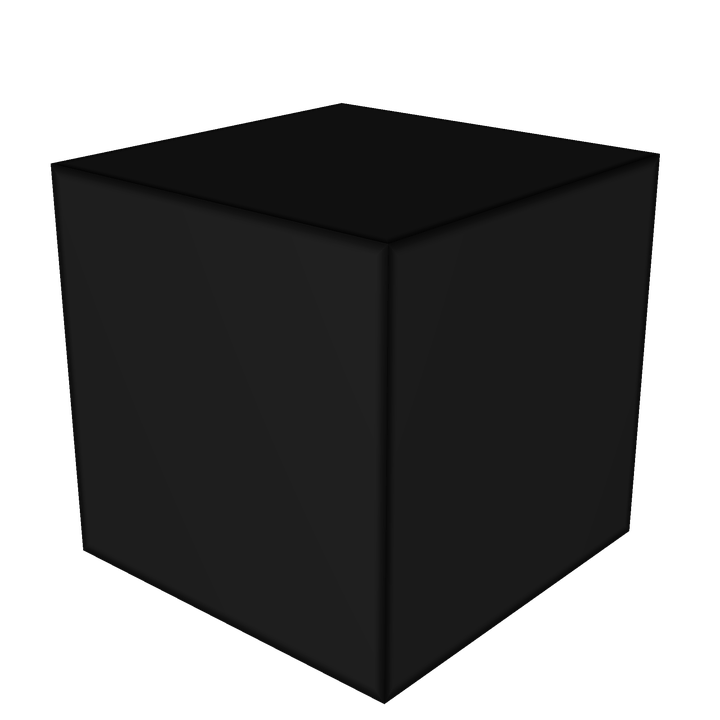
\includegraphics[width=106.5pt,height=104.25pt]{w07_hpo_grey_box/images/intro/black_box.png}};

% Text Node
\draw (284,106.5) node   [align=left] { \textcolor[rgb]{1,1,1}{{\Huge ?}}};
% Text Node
\draw (39,104) node   [align=left] {\textcolor[rgb]{1,1,1}{X}};
% Text Node
\draw (586,102) node   [align=left] {\textcolor[rgb]{1,1,1}{f(X)}};
% Text Node
\draw (317,28) node   [align=left] {Objective function};
% Text Node
\draw (309,254) node   [align=left] {Only interaction: Query of function at $\displaystyle \conf$ to obtain $\displaystyle \cost(\conf)$};


\end{tikzpicture}

\end{figure}
\pause
\begin{itemize}
    \item Can we do better?
\end{itemize}
%\source{\lit{\href{https://slideslive.com/38917532/greybox-bayesian-optimization-for-automl}{Peter Frazier: Grey-box Bayesian Optimization for AutoML}}}
    
    \textcolor{red}{FH: can you please create this figure yourself, using the same picture for black box and looking inside the black box, except that for ``looking inside'' the lid is open. For one (not necessarily optimal) way to do this in tikz, see: http://www.texample.net/tikz/examples/annotated-3d-box/}
    
\end{frame}
%-------------------------------------------------




%\section{Introduction to grey-box approaches}
%-------------------------------------------------
%-------------------------------------------------
\begin{frame}{Recall: Black-box optimization}
\begin{figure}
    \centering
    


\tikzset{every picture/.style={line width=0.75pt}} %set default line width to 0.75pt        

\begin{tikzpicture}[x=0.70pt,y=0.70pt,yscale=-1,xscale=1]
%uncomment if require: \path (0,300); %set diagram left start at 0, and has height of 300

%Straight Lines [id:da5075678478287002] 
\draw    (74.5,104) -- (218.5,104) ;
\draw [shift={(220.5,104)}, rotate = 180] [color={rgb, 255:red, 0; green, 0; blue, 0 }  ][line width=0.75]    (10.93,-3.29) .. controls (6.95,-1.4) and (3.31,-0.3) .. (0,0) .. controls (3.31,0.3) and (6.95,1.4) .. (10.93,3.29)   ;
%Shape: Square [id:dp6368535923226633] 
\draw  [fill={rgb, 255:red, 0; green, 25; blue, 255 }  ,fill opacity=1 ] (14,79) -- (64,79) -- (64,129) -- (14,129) -- cycle ;
%Shape: Square [id:dp8011400143211207] 
\draw  [fill={rgb, 255:red, 0; green, 25; blue, 255 }  ,fill opacity=1 ] (561,79) -- (611,79) -- (611,129) -- (561,129) -- cycle ;
%Straight Lines [id:da6772752516220095] 
\draw    (401.5,101) -- (540.5,101.99) ;
\draw [shift={(542.5,102)}, rotate = 180.41] [color={rgb, 255:red, 0; green, 0; blue, 0 }  ][line width=0.75]    (10.93,-3.29) .. controls (6.95,-1.4) and (3.31,-0.3) .. (0,0) .. controls (3.31,0.3) and (6.95,1.4) .. (10.93,3.29)   ;
%Straight Lines [id:da7102938160527976] 
\draw    (39.5,242) -- (39.01,143) ;
\draw [shift={(39,141)}, rotate = 449.72] [color={rgb, 255:red, 0; green, 0; blue, 0 }  ][line width=0.75]    (10.93,-3.29) .. controls (6.95,-1.4) and (3.31,-0.3) .. (0,0) .. controls (3.31,0.3) and (6.95,1.4) .. (10.93,3.29)   ;
%Straight Lines [id:da5275375794470956] 
\draw    (39.5,242) -- (123.5,242) ;
%Straight Lines [id:da11206880859629287] 
\draw    (123.5,242) -- (586.5,242) ;
%Straight Lines [id:da8957848321230528] 
\draw    (586.5,135) -- (586.5,242) ;
%Image [id:dp5678753924043267] 
\draw (313.5,101.5) node  {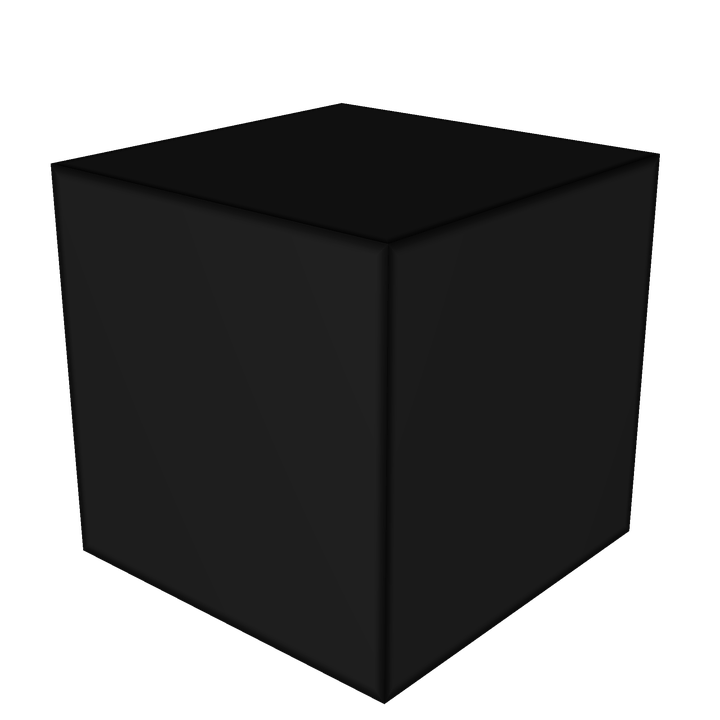
\includegraphics[width=106.5pt,height=104.25pt]{w07_hpo_grey_box/images/intro/black_box.png}};

% Text Node
\draw (284,106.5) node   [align=left] { \textcolor[rgb]{1,1,1}{{\Huge ?}}};
% Text Node
\draw (39,104) node   [align=left] {\textcolor[rgb]{1,1,1}{X}};
% Text Node
\draw (586,102) node   [align=left] {\textcolor[rgb]{1,1,1}{f(X)}};
% Text Node
\draw (317,28) node   [align=left] {Objective function};
% Text Node
\draw (309,254) node   [align=left] {Only interaction: Query of function at $\displaystyle \conf$ to obtain $\displaystyle \cost(\conf)$};


\end{tikzpicture}

\end{figure}
\pause
\begin{itemize}
    \item Can we do better?
\end{itemize}
%\source{\lit{\href{https://slideslive.com/38917532/greybox-bayesian-optimization-for-automl}{Peter Frazier: Grey-box Bayesian Optimization for AutoML}}}
    
    \textcolor{red}{FH: can you please create this figure yourself, using the same picture for black box and looking inside the black box, except that for ``looking inside'' the lid is open. For one (not necessarily optimal) way to do this in tikz, see: http://www.texample.net/tikz/examples/annotated-3d-box/}
    
\end{frame}
%-------------------------------------------------
%-------------------------------------------------
\begin{frame}{Looking inside the box}
\begin{figure}
    \centering
    


\tikzset{every picture/.style={line width=0.75pt}} %set default line width to 0.75pt        

\begin{tikzpicture}[x=0.70pt,y=0.70pt,yscale=-1,xscale=1]
%uncomment if require: \path (0,300); %set diagram left start at 0, and has height of 300

%Straight Lines [id:da5075678478287002] 
\draw    (74.5,104) -- (218.5,104) ;
\draw [shift={(220.5,104)}, rotate = 180] [color={rgb, 255:red, 0; green, 0; blue, 0 }  ][line width=0.75]    (10.93,-3.29) .. controls (6.95,-1.4) and (3.31,-0.3) .. (0,0) .. controls (3.31,0.3) and (6.95,1.4) .. (10.93,3.29)   ;
%Shape: Square [id:dp6368535923226633] 
\draw  [fill={rgb, 255:red, 0; green, 25; blue, 255 }  ,fill opacity=1 ] (14,79) -- (64,79) -- (64,129) -- (14,129) -- cycle ;
%Shape: Square [id:dp8011400143211207] 
\draw  [fill={rgb, 255:red, 0; green, 25; blue, 255 }  ,fill opacity=1 ] (561,79) -- (611,79) -- (611,129) -- (561,129) -- cycle ;
%Straight Lines [id:da6772752516220095] 
\draw    (401.5,101) -- (540.5,101.99) ;
\draw [shift={(542.5,102)}, rotate = 180.41] [color={rgb, 255:red, 0; green, 0; blue, 0 }  ][line width=0.75]    (10.93,-3.29) .. controls (6.95,-1.4) and (3.31,-0.3) .. (0,0) .. controls (3.31,0.3) and (6.95,1.4) .. (10.93,3.29)   ;
%Straight Lines [id:da7102938160527976] 
\draw    (39.5,242) -- (39.01,143) ;
\draw [shift={(39,141)}, rotate = 449.72] [color={rgb, 255:red, 0; green, 0; blue, 0 }  ][line width=0.75]    (10.93,-3.29) .. controls (6.95,-1.4) and (3.31,-0.3) .. (0,0) .. controls (3.31,0.3) and (6.95,1.4) .. (10.93,3.29)   ;
%Straight Lines [id:da5275375794470956] 
\draw    (39.5,242) -- (123.5,242) ;
%Straight Lines [id:da11206880859629287] 
\draw    (123.5,242) -- (586.5,242) ;
%Straight Lines [id:da8957848321230528] 
\draw    (586.5,135) -- (586.5,242) ;
%Image [id:dp9410017568713034] 
\draw (307.5,95) node  {
\includegraphics[width=94.5pt,height=76.5pt]{w07_hpo_grey_box/images/intro/opened_box.png}};
%Straight Lines [id:da7498039648909043] 
\draw    (264,72) -- (222.18,45.08) ;
\draw [shift={(220.5,44)}, rotate = 392.77] [color={rgb, 255:red, 0; green, 0; blue, 0 }  ][line width=0.75]    (10.93,-3.29) .. controls (6.95,-1.4) and (3.31,-0.3) .. (0,0) .. controls (3.31,0.3) and (6.95,1.4) .. (10.93,3.29)   ;

% Text Node
\draw (39,104) node   [align=left] {\textcolor[rgb]{1,1,1}{X}};
% Text Node
\draw (586,102) node   [align=left] {\textcolor[rgb]{1,1,1}{f(X)}};
% Text Node
\draw (317,28) node   [align=left] {Objective function};
% Text Node
\draw (309,254) node   [align=left] {Only interaction: Query of function at $\displaystyle \conf$ to obtain $\displaystyle \cost(\conf)$};
% Text Node
\draw (158,38) node   [align=left] {other information};


\end{tikzpicture}

\end{figure}

    \textcolor{red}{FH: can you please create this figure yourself, using the same picture for black box and looking inside the black box, except that for ``looking inside'' the lid is open. For one (not necessarily optimal) way to do this in tikz, see: http://www.texample.net/tikz/examples/annotated-3d-box/}

%\hspace{6.5cm}\lit{\href{https://slideslive.com/38917532/greybox-bayesian-optimization-for-automl}{Peter Frazier: Grey-box Bayesian Optimization for AutoML}}
\end{frame}
%-------------------------------------------------


\begin{frame}{Looking inside the box}
Utilize additional knowledge available about the objective function to improve optimization performance:
\begin{itemize}
    \item Learning curves:
    \begin{itemize}
        \item Early stopping
        \item Freezing \& Thawing
    \end{itemize}
    \item Cheap-to-evaluate proxies
    \begin{itemize}
        \item Trained neural network on small part of $\dataset$ 
    \end{itemize}
    \item Multi-task learning
    \begin{itemize}
        \item Solve multiple learning tasks simultaneously.
        \item Exploit commonalities and differences across tasks.
    \end{itemize}
    \item Warm starts
    \begin{itemize}
        \item Reuse trained hyperparameter configurations from similar models or datasets.
    \end{itemize}
\end{itemize}
\end{frame}
%-------------------------------------------------
%-------------------------------------------------
%\iffalse
\begin{frame}{Learning Curves}

\centering
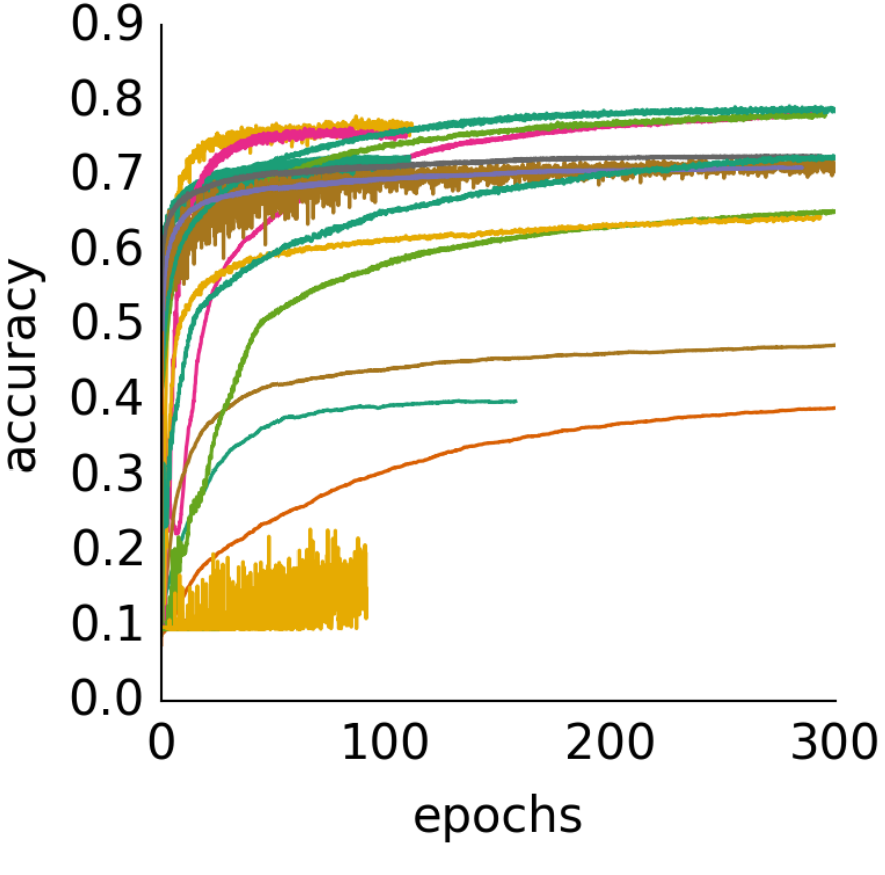
\includegraphics[width=0.4\textwidth]{w07_hpo_grey_box/images/intro/learning_curves.png}

Exemplary learning curves of training deep neural networks\\
Many ML algorithms iteratively optimize a (loss) function

\end{frame}
%-------------------------------------------------
%-------------------------------------------------
\begin{frame}{Stopping poor evaluations early}

\centering
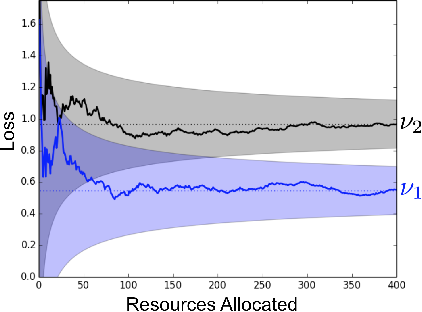
\includegraphics[width=0.5\textwidth]{w07_hpo_grey_box/images/intro/differetiatingConfigurations.png}

Only stop evaluations after they have spent sufficient resources to differentiate between them in terms of quality.

\end{frame}
\fi
%\videotitle{Meta-Learning}
%----------------------------------------------------------------------

\begin{frame}[c]{Introduction}

\notefh{Please add the visualization on the first slide for meta-learning}

\begin{itemize}
	\item Learning essentially never stops:
	\begin{itemize}
		\item Many models are periodically re-fit to track changes in the data
		\item Many models are re-fit to perform well on new tasks
	\end{itemize}
	
    \item Machine Learning is often done from scratch
    
    \item We humans do not start from scratch all the time \\ - we learned how to learn!
\end{itemize}

\end{frame}
% %----------------------------------------------------------------------
% %----------------------------------------------------------------------
% \begin{frame}[c]{Meta-Learning}
% \framesubtitle{Introduction}

% \begin{columns}
% 	\column{0.18\textwidth}
% 	Ren\'e Magritte
% 	\centering
% 	
\includegraphics[width=.9\textwidth]{../w07_hpo_speedup/images/meta_learning/magritte_1.jpg}
% 	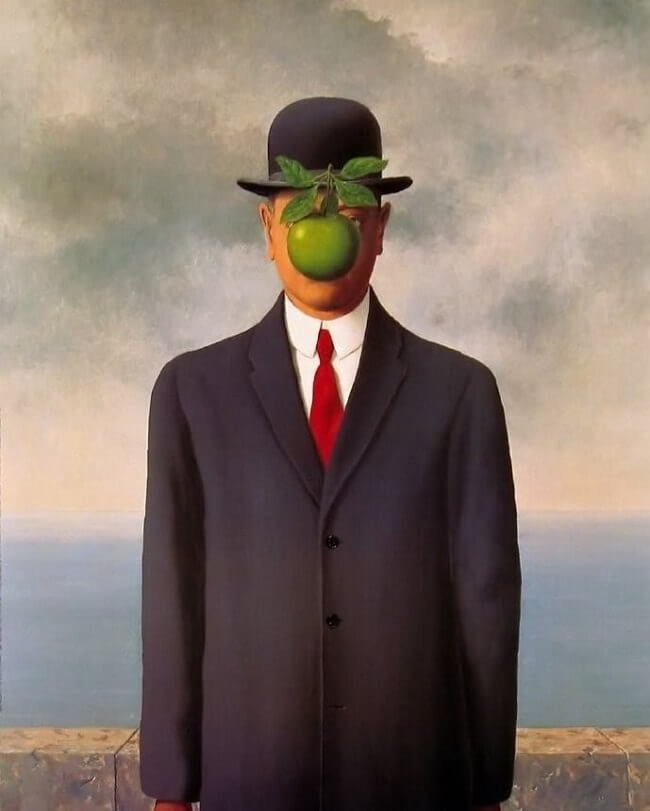
\includegraphics[width=.9\textwidth]{../w07_hpo_speedup/images/meta_learning/magritte_2.jpg}
% 	\column{0.258\textwidth}
% 	Francis Picabia
% 	\centering
% 	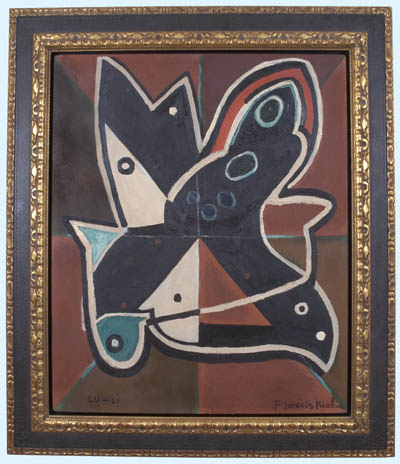
\includegraphics[width=.7\textwidth]{../w07_hpo_speedup/images/meta_learning/picabia_3.jpg}
% 	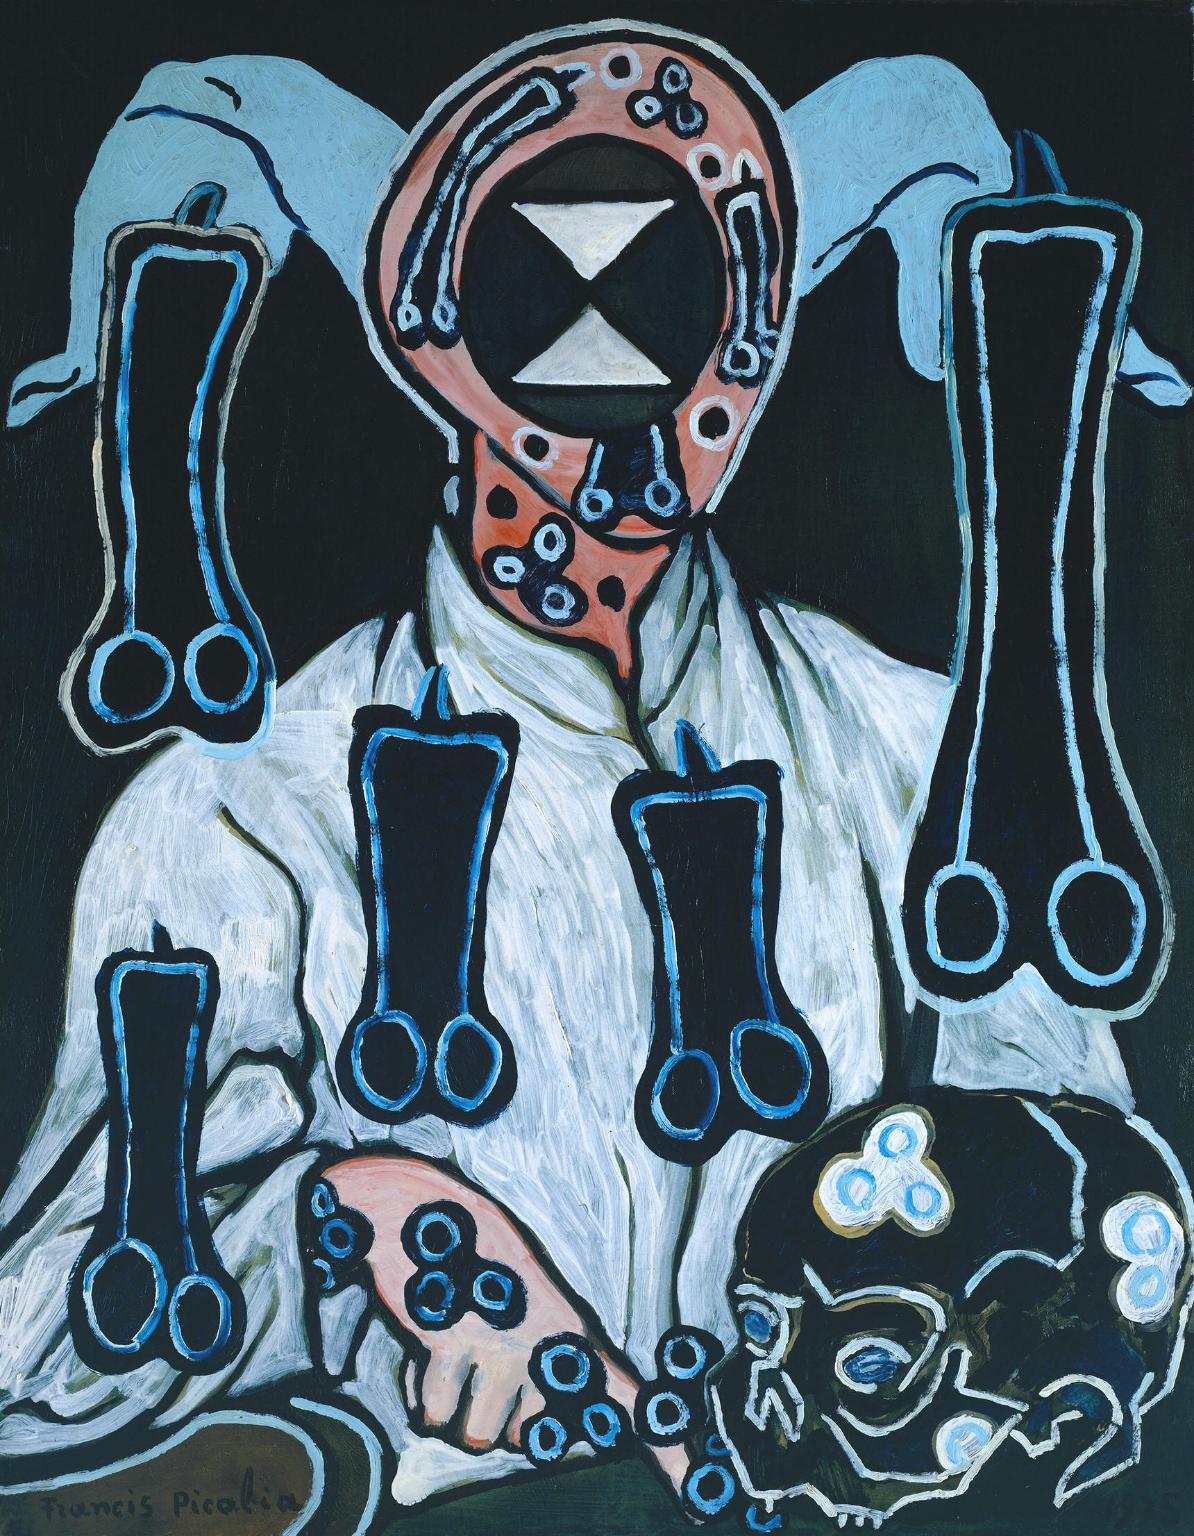
\includegraphics[width=.6\textwidth]{../w07_hpo_speedup/images/meta_learning/picabia_1.jpg}
% 	\column{0.3\textwidth}
% 	\centering
% 	Who painted that?
% 	
\includegraphics[width=.7\textwidth]{../w07_hpo_speedup/images/meta_learning/magritte_3.jpg}
	
% 	\pause
% 	Most likely most of you can identify the painter correctly, 
% 	although I presented only two pictures of each.
% \end{columns}

% \end{frame}
% % %----------------------------------------------------------------------
% % %----------------------------------------------------------------------

%----------------------------------------------------------------------
%----------------------------------------------------------------------
\begin{frame}[c]{Learning from model evaluations}

\begin{itemize}
    \item Similarly, while building ML models for a specific task, we exploit our experience with related tasks
    \item The challenge of meta-learning is to provide a systematic and data-driven approach to learn from experience 
    \item Consider that we have an access to:
        \begin{itemize}
            \item set of prior tasks: $t_{j} \in \mathcal{T}$,
            \item set of new tasks: $t_{\text{new}} \in \mathcal{T}$,
            \item set of learning algorithms, fully defined by $\theta_{i} \in \Theta$
            \item set of prior evaluations: $\dataset$, where $\dataset_{i, j} = \cost(\theta_{i}, t_{j})$
            \begin{itemize}
                \item $\dataset_{\text{new}}$ is the set of known evaluations $\cost_{i, \text{new}}$ on a new task $t_{\text{new}}$
            \end{itemize}
        \end{itemize}
    \item \emph{Goal.} Train a meta-learner using meta-data $\dataset \cup \dataset_{\text{new}}$, such that it recommends configurations for a new task better than a black-box algorithm
\end{itemize}

\hspace{11cm}\lit{\href{https://www.springer.com/gp/book/9783030053178}{AutoML Book: Chapter 2}}

\end{frame}
% %----------------------------------------------------------------------
% %----------------------------------------------------------------------

%----------------------------------------------------------------------
%----------------------------------------------------------------------
\begin{frame}[c]{Learning from task properties}

\begin{itemize}
    \item Other than characterize the data by its performance, we can extract characterizations (called \alert{meta-features}) from data at hand 
    \item Each task $t_j$ can be described by a vector of $K$ meta-features:
        \begin{equation*}
            m(t_j) = (m_{j, 1}, \dots, m_{j, K})
        \end{equation*}
    \item This vector can be used to define the similarity measure between two tasks, e.g. calculating the Euclidean distance between $m(t_i)$ and $m(t_j)$
    \item Based on similarity, we can transfer information from the most similar tasks to the new task $t_{\text{new}}$
    \end{itemize}

\hspace{11cm}\lit{\href{https://www.springer.com/gp/book/9783030053178}{AutoML Book: Chapter 2}}

\end{frame}
% %----------------------------------------------------------------------
% %----------------------------------------------------------------------

% \begin{frame}[c]{Meta-Learning}
% \framesubtitle{Supervised Learning revisited}

% Dataset:
% \begin{equation*}
% \dataset = \{(x_1, y_1), \ldots, (x_k, y_k) \}
% \end{equation*}

% \bigskip
% \pause

% Learning a model $\phi$ (e.g., weights of a neural network):
% \begin{eqnarray*}
% \argmax_{\phi} \log p(\phi|\dataset)\\
% \pause
% = \argmax_{\phi} \log p(\dataset | \phi) + \log p(\phi) \\
% \pause
% = \argmax_{\phi} \sum_i \log p(y_i | x_i, \phi) + \log p(\phi)
% \end{eqnarray*}

% \pause

% Challenge:
% \begin{itemize}
% 	\item Learning starts from scratch
% 	\item We might only have very few examples in $\dataset$ 
% \end{itemize}

% \end{frame}
% %----------------------------------------------------------------------
% %----------------------------------------------------------------------
% \begin{frame}[c]{Meta-Learning}
% \framesubtitle{Problem formulation}

% Dataset:
% \begin{equation*}
% \dataset = \{(x_1, y_1), \ldots, (x_k, y_k) \}
% \end{equation*}
% Set of datasets (meta-datasets):
% \begin{equation*}
% \mdata = \{\mathcal{D}_1, \ldots, \mathcal{D}_n, \}
% \end{equation*}

% \pause
% Can we include these meta-datasets to improve learning on $\dataset$?
% \begin{equation*}
% \argmax_{\phi} \log p(\phi|\dataset, \mdata)
% \end{equation*}

% \pause
% \medskip

% \alert{Idea:} Instead of keeping $\mdata$ forever, we want to distill the knowledge into \alert{meta-parameters $\theta$}: $p(\theta|\mdata)$
 
% \end{frame}
% %----------------------------------------------------------------------
% %----------------------------------------------------------------------
% \begin{frame}[c]{Meta-Learning}
% \framesubtitle{Problem formulation}

% In meta-learning, we want to learn:
% \begin{eqnarray*}
% \argmax_{\phi} \log p(\phi|\dataset, \mdata) \\
% \pause
% = \argmax_{\phi} \log \int_{\Theta} p(\phi \mid \dataset, \theta) p(\theta \mid \mdata) d\theta\\
% \pause
% \approx \argmax_{\phi} \log p(\phi | \dataset, \theta^*) + \log p(\theta^* | \mdata)\\
% \pause
% = \argmax_{\phi} \log p(\phi | \dataset, \theta^*)
% \end{eqnarray*}

% \pause

% \begin{center}
% \begin{minipage}{0.5\textwidth}
% \begin{block}{Meta-learning problem}
% \begin{equation*}
% \theta^* \in \argmax_{\theta} \log p(\theta | \mdata)
% \end{equation*}
% \end{block}
% \end{minipage}
% \end{center}

% \end{frame}
% %-----------------------------------------------------------------------
% %-----------------------------------------------------------------------
% \begin{frame}[c]{Meta-Learning}
% \framesubtitle{AutoML $\subset$ Meta-Learning}

% \begin{itemize}
% 	\item AutoML can be seen as a special case of meta-learning \pause
% 	\medskip
% 	\item $\theta$ could be:
% 	\begin{itemize}
% 		\item a hyperparameter configuration ($\lambda$) 
% 		\item a neural network architecture
% 	\end{itemize}
% 	\pause
% 	\medskip
% 	\item What would be $\mdata$ here? 
% 	\pause
% 	\begin{itemize}
% 		\item A dataset on which we optimized $\lambda$ (e.g. CIFAR-10)\\ such that we can use it on another dataset (e.g. imagenet)
% 	\end{itemize}
% \end{itemize}	

% \end{frame}
% %-----------------------------------------------------------------------
% %-----------------------------------------------------------------------
% \begin{frame}[c]{Meta-Learning}
% \framesubtitle{Meta-Learning $\subset$ AutoML}

% \begin{itemize}
% 	\item Meta-learning can be powerful to complement AutoML
% 	\pause
% 	\medskip
% 	\item We can learn a lot of things from $\mdata$ to improve the performance on new datasets, e.g.:
% 	\begin{itemize}
% 		\item pre-initialization of networks weights
% 		\item learning a meta-DNN to predict how to train another target-DNN	\end{itemize}
% \end{itemize}	

% \end{frame}
%-----------------------------------------------------------------------
%-----------------------------------------------------------------------
\begin{frame}[c]{Meta-Features in Machine Learning}

\begin{itemize}
	\item \alert{Simple} - easily extracted from the data, describe the basic dataset structure: e.g. number of features, patterns or classes. \pause
	
	\item \alert{Statistical} - characterize the data via descriptive statistics: e.g. average, standard deviation, correlation, the kurtosis or the dispersion of the label distribution. \pause
	
	\item \alert{Information-theoretic} - measure the class entropy in the data, capturing the amount of information in the data and their complexity. \pause 
    
    \item \alert{Model-based} - extracted from a model induced using the training data, they are often based on properties of decision tree models: e.g. the number of leaves, the number of nodes, the shape of the tree. \pause
		
	\item \alert{Landmarking} - computed by running several fast machine learning algorithms on the dataset. Based on their learning scheme they can capture different properties of the dataset, like e.g. linear separability. \pause
	
	\item \alert{Others} - not included in the previous groups, such as standalone measures, time related measures, concept and case-based measures, clustering and distance-based measures.
	
\end{itemize}

\end{frame}
%-----------------------------------------------------------------------
%-----------------------------------------------------------------------
\begin{frame}[c]{Warmstarting}
	
\begin{itemize}
	\item Recap: Instead of starting from a random configuration we often start from a expert-defined configuration for hyperparameter optimization (HPO)
	\pause
	\item We also know that such a default configuration often does not perform well on a new dataset
	\begin{itemize}
		\item Otherwise there would be no point in HPO
	\end{itemize}
	\pause
	\item \alert{Can we learn from previous datasets $\mdata$ how to initialize HPO?}\\
	(i.e., running an initial design)
%	\begin{itemize}
%		\item the same ideas also apply to NAS
%		\item for simplicity we focus on HPO 
%	\end{itemize}
\end{itemize}

\end{frame}
%-----------------------------------------------------------------------
%----------------------------------------------------------------------
%----------------------------------------------------------------------
\begin{frame}[c]{Model-Warmstarting}

\begin{itemize}
	\item Many HPO optimizers make use of some kind of a predictive model,\\
	e.g., Bayesian optimization
	\item By running HPO over and over again on different datasets,
	we can actually learn something about the search landscape
	\begin{itemize}
		\item E.g., what are bad regions of the configuration space in general
	\end{itemize}
	\smallskip
	\item Given: $n$ predictive models $\surro_{\dataset_i}: \pcs \to \mathbb{R}$ from HPO on $\dataset_{\text{meta}}$	
	\item \alert{How can we use these $\surro_{\dataset_i}$ to speed up HPO?}
\end{itemize}


\end{frame}
%-----------------------------------------------------------------------

%-----------------------------------------------------------------------
%-----------------------------------------------------------------------
\begin{frame}[c]{Task-independent Recommendations}

\begin{columns}[T] % align columns
\begin{column}{.48\textwidth}

    \only<1->{
    \begin{itemize}
        \item \emph{Idea:} learn a sorted list of defaults
        \item \emph{Method:} mostly greedy 
        \item \emph{Results:} improves over Random Search and Bayesian Optimization
    \end{itemize}}

    \only<2->{
    \begin{block}{Advantages}
    \begin{itemize}
    	\item Easy to share and use
    	\item Strong anytime performance
    	\item Embarrassingly parallel
    \end{itemize}
    \end{block}}
    
    \only<2->{
    \begin{block}{Disadvantages}
    \begin{itemize}
    	\item Not adaptive
    \end{itemize}
    \end{block}}

\end{column}%

\hfill%

\begin{column}{.48\textwidth}

    \centering
    \onslide<1->{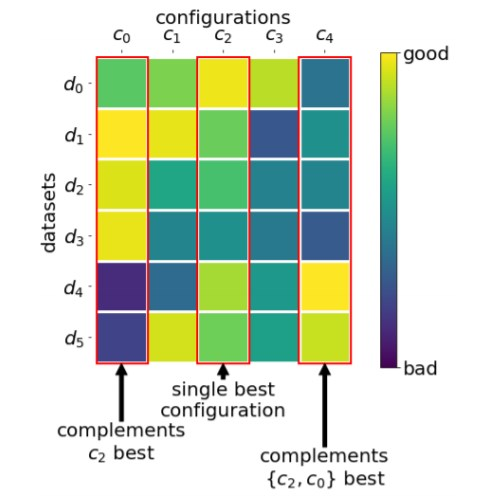
\includegraphics[width=.8\textwidth]{../w07_hpo_speedup/images/meta_learning/task_independent.jpg}}
%    \only<2->{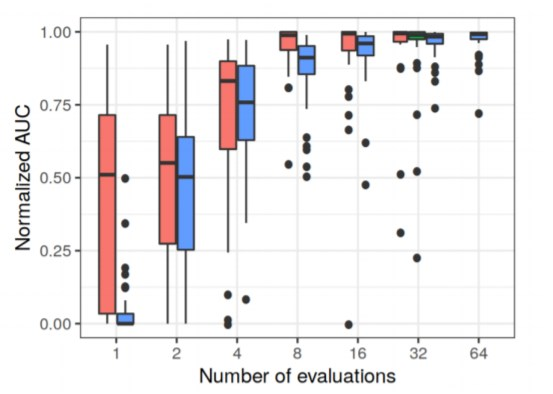
\includegraphics[width=.9\textwidth]{../w07_hpo_speedup/images/meta_learning/task_independent_results.jpg}}


\end{column}
\end{columns}  



\vspace{0.5cm}
\hspace{6cm}
\lit{\href{https://link.springer.com/article/10.1007/s10994-017-5684-y}{Wistuba et al. 2015a}}, \lit{\href{https://arxiv.org/pdf/1802.02219.pdf}{Feurer et al. 2018}},  \lit{\href{}{Pfisterer et al. 2018}}



\end{frame}
%-----------------------------------------------------------------------
%-----------------------------------------------------------------------

%-----------------------------------------------------------------------
%-----------------------------------------------------------------------
\begin{frame}[c]{Joint model for Bayesian optimization}

\begin{columns}[T] % align columns
\begin{column}{.38\textwidth}

\begin{itemize}
    \item<1-> Jointly train a „deep“ neural network on all tasks 
    \item<2-> Have a separate output layer (head) for each tasks 
    \item<3-> Each head is a Bayesian linear regression 
    \item<4-> Feature extraction on hyperparameter configurations 
    \item<5-> (Recall DNGO)
\end{itemize}
\end{column}%

\hfill%

\begin{column}{.58\textwidth}
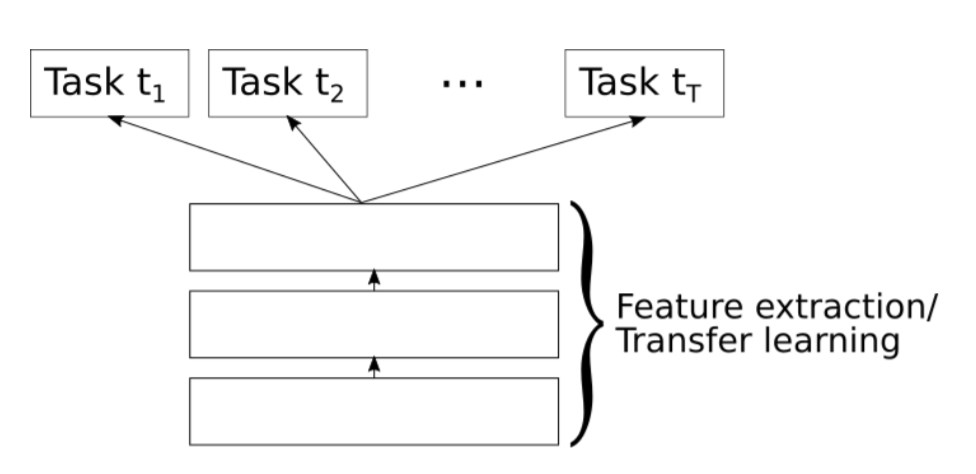
\includegraphics[width=0.9\textwidth]{../w07_hpo_speedup/images/meta_learning/perrone_int.jpg}
\end{column}%
\end{columns}

\hspace{12cm}\lit{\href{http://papers.nips.cc/paper/7917-scalable-hyperparameter-transfer-learning.pdf}{Perrone et al. 2018}}

\end{frame}
%-----------------------------------------------------------------------
%-----------------------------------------------------------------------
%\begin{frame}[c]{Joint model for Bayesian optimization}
%
%\centering
%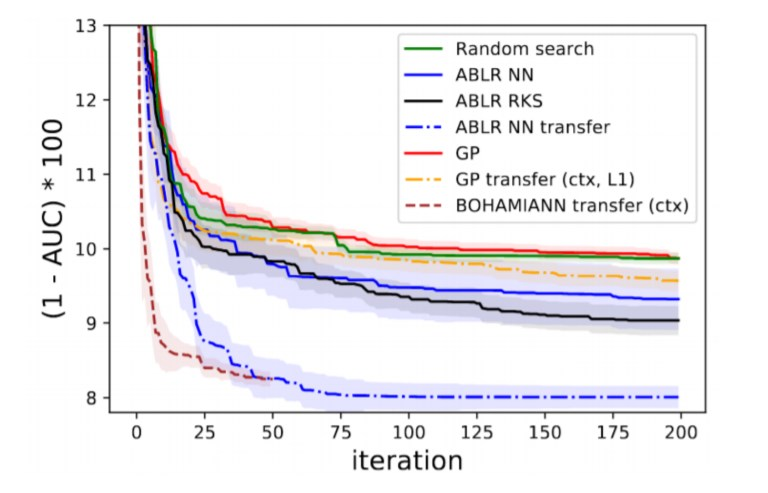
\includegraphics[width=0.7\textwidth]{../w07_hpo_speedup/images/meta_learning/perrone_res.jpg}
%
%\end{frame}
%-----------------------------------------------------------------------
%-----------------------------------------------------------------------

%----------------------------------------------------------------------
%----------------------------------------------------------------------
\begin{frame}[c]{Learning a Black-box Optimization Algorithm from Data}

\myit{

    \item Recall the black box optimization setting:
    \begin{enumerate}
        \item Given the current state of knowledge $\iter[\bocount]{h}$, propose the next query point $\iter[\bocount]{x}$
        \item Observe the response $\iter[\bocount]{y}$ \& update any internal statistics to produce $\iter[\bocount+1]{h}$
    \end{enumerate}
    
    \pause
    \bigskip
    
    \item \alert{Learning} a blackbox optimization algorithm
    \myit{
        \item Learn a mapping from $\iter[\bocount]{h}$ to next query $\iter[\bocount]{x}$
        \item This mapping can be a (recurrent) neural net $\text{NN}_{\phi}: \iter[\bocount]{h} \mapsto \iter[\bocount]{x}$ parameterized by weights $\phi$   
\pause        
        \item \alert{This mapping $\text{NN}_{\phi}$ constitutes a blackbox optimization algorithm}
        \myit{
            \item Should be learned on a \alert{meta-train} set of blackbox functions \& generalize to new functions
%            \item Like a manually-designed algorithm ...
        }

%\pause
%        \item Since $\iter[\bocount]{h}$ captures a \alert{sequence}, a recurrent NN $RNN_{\phi}:\iter[\bocount]{h} \mapsto \iter[\bocount]{x}$ makes sense

\pause
\bigskip
    
    }
    
    \item Existing approaches for learning a blackbox optimizer
    \myit{
        \item \alert{Gradient descent} on $\phi$  \lit{\href{http://proceedings.mlr.press/v70/chen17e.html}{Chen et al. 2017}}
        \myit{
            \item Simplest technique, but requires backpropagation through the optimization trace
            \item This also requires the blackbox functions $f$ used for training to be differentiable
       }
        \item \alert{Reinforcement learning} \lit{\href{https://arxiv.org/abs/1606.01885}{Li \& Malik, 2016}}
        \myit{
            \item Can be harder to get to work, but does not require differentiable $f$
        }
    
%        \item Gradient-free approaches should also work

    }
}

\end{frame}
%----------------------------------------------------------------------
%----------------------------------------------------------------------
%-----------------------------------------------------------------------
%-----------------------------------------------------------------------
\begin{frame}[c]{Learning Acquisition Functions}

\begin{itemize}
	\item Learning a complete optimization algorithm  \alert{requires a lot of data}
	\item A more \alert{sample-efficient} would be to \alert{only replace hand-designed parts} of an algorithm

\bigskip
\pause
	\item In Bayesian optimization, a critical hand-designed heuristic is the acquisition function
	\begin{itemize}
		\item Trade-off between exploitation and exploration
		\item Depending on the problem at hand, you might need a different acquisition function
		\pause
		\item Choices: PI, EI, UCB, ES, KG, \dots 
		%all of them are \alert{myopic} (no long-term look-ahead)
	\end{itemize}
\pause
\bigskip

    \item \alert{Idea:} Learn a \alert{neural acquisition function} from data, but still make use of the sample efficiency of Gaussian processes \lit{\href{https://openreview.net/forum?id=ryeYpJSKwr}{Volpp et al. 2020}}

\pause
\medskip
    \item Two options:
    \myit{
        \item Only depend on predicted mean and variance: $\acq_\theta(x) = \acq_\theta(\mu_t(x), \sigma_t(x))$ 
        \myit{
            \item This allows to learn a general acquisition function
        }
        \item Also depend on the $x$ value: $\acq_\theta(x) = \acq_\theta(\mu_t(x), \sigma_t(x), \alert{x})$  
    }

\end{itemize}


\end{frame}
%-----------------------------------------------------------------------

%-----------------------------------------------------------------------
\begin{frame}[c]{Questions to Answer for Yourself / Discuss with Friends}

\begin{itemize}
    \item \alert{Repetition.} What are the different kind of meta-features which can be used to describe machine learning datasets?
    
    \medskip

    \item \alert{Discussion.}
    \begin{itemize}
        \item How would you pick meta-features to be used in meta-learning hyperparameter optimization?
        \item What will happen with the meta-learning system if all prior tasks are dissimilar to the target task?
    \end{itemize}
\end{itemize}

\end{frame}
%\section{Learning Curve Prediction}
\begin{frame}{Learning Curves}
\notefh{Please add the visualization on the first slide}

\begin{figure}
   \centering
   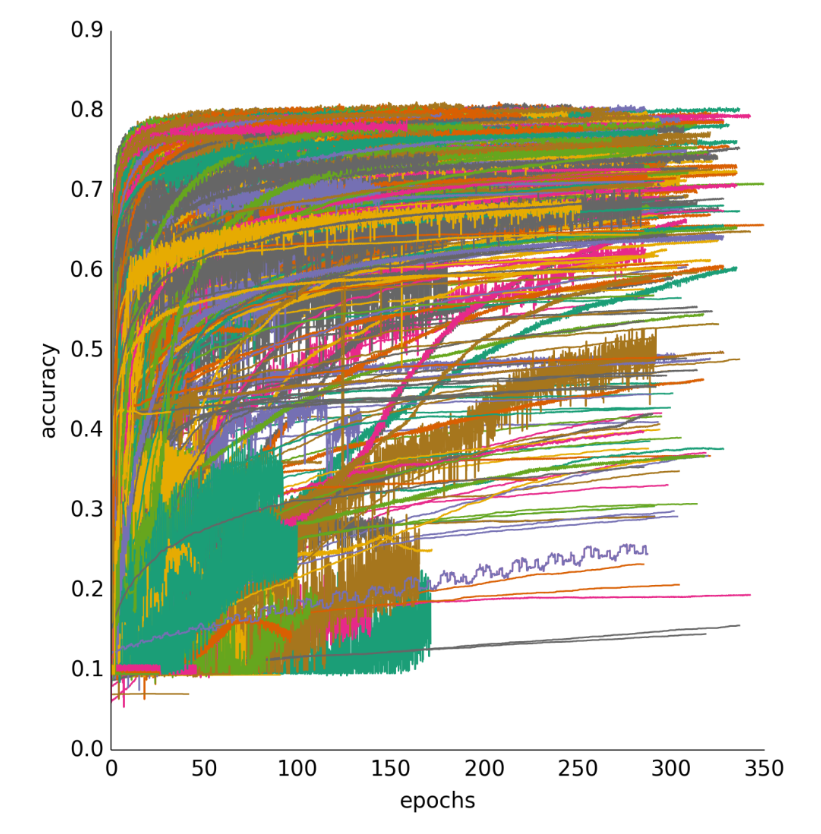
\includegraphics[width=0.44\textwidth]{w07_hpo_grey_box/images/learningcurve/learning_curve_domhan.png}
   \caption{Exemplary learning curves of training deep neural networks}
\end{figure}




\end{frame}
%-----------------------------------------------------------------------

%-----------------------------------------------------------------------
\begin{frame}{Learning Curve Predictions}
\onslide<1->
\begin{figure}
    \centering
    \only <1>{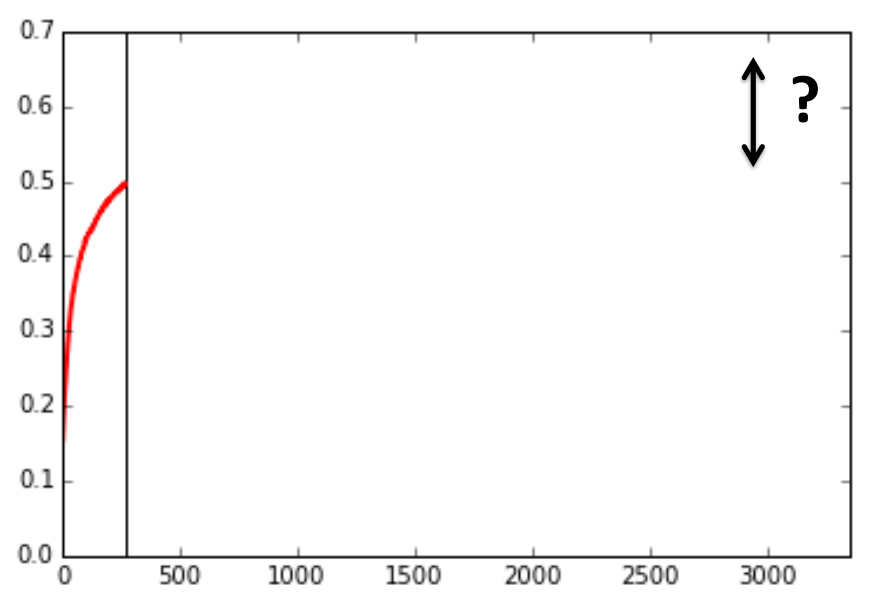
\includegraphics[width=0.5\textwidth]{w07_hpo_grey_box/images/learningcurve/learning_curve_questionmark.png}}
    \only <2->{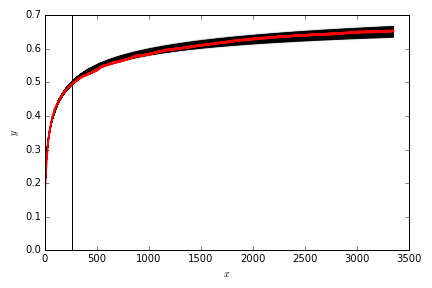
\includegraphics[width=0.5\textwidth]{w07_hpo_grey_box/images/learningcurve/learning_curve_single_pred.jpg}}
    
\end{figure}


\begin{enumerate}
  \item Observe learning curve for the first $n$ steps (here $n=250$)
  \pause
  \item \alert{Extrapolation}: fit parametric model on partial learning curve to predict remaining learning curve
  \pause
  \begin{itemize}
      \item Various models can be used (see following slides) 
  \end{itemize}
  
 % Which model to use? E.g.,
 % \begin{itemize}
%	\item Parametric density models: give table with equations
%	\item Neural network with learning curve layer
%	\item Recurrent neural network
%%    \item Good model depends on shape of curve $\to$ e.$\,$g., depends on optimizer  
%%    \item[$\leadsto$] combination of several models
%  \end{itemize}
  
\end{enumerate}

\end{frame}
%-----------------------------------------------------------------------

%-----------------------------------------------------------------------
\begin{frame}{Learning Curves: Early Termination}

\centering
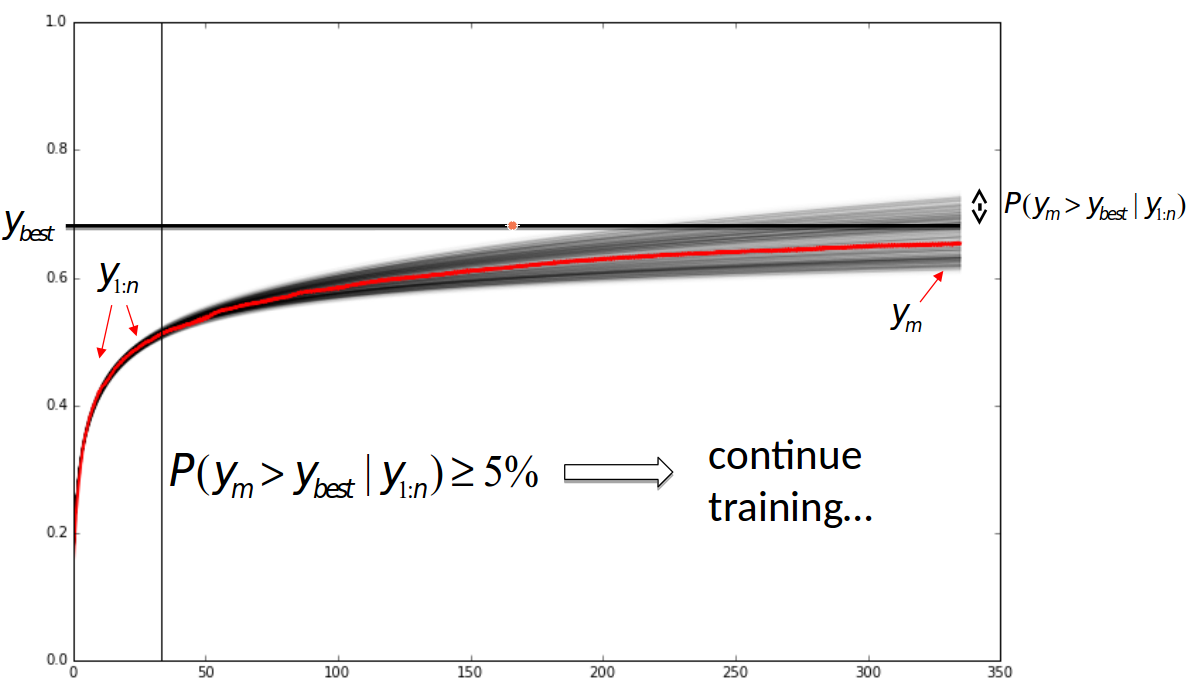
\includegraphics[width=0.8\textwidth]{w07_hpo_grey_box/images/learningcurve/learning_curve_dec.png}

$\rightarrow$ need for \alert{probabilistic predictions / quantification of uncertainty}

\end{frame}
%-----------------------------------------------------------------------
%-----------------------------------------------------------------------
\begin{frame}{Learning Curves: Early Termination}

\centering
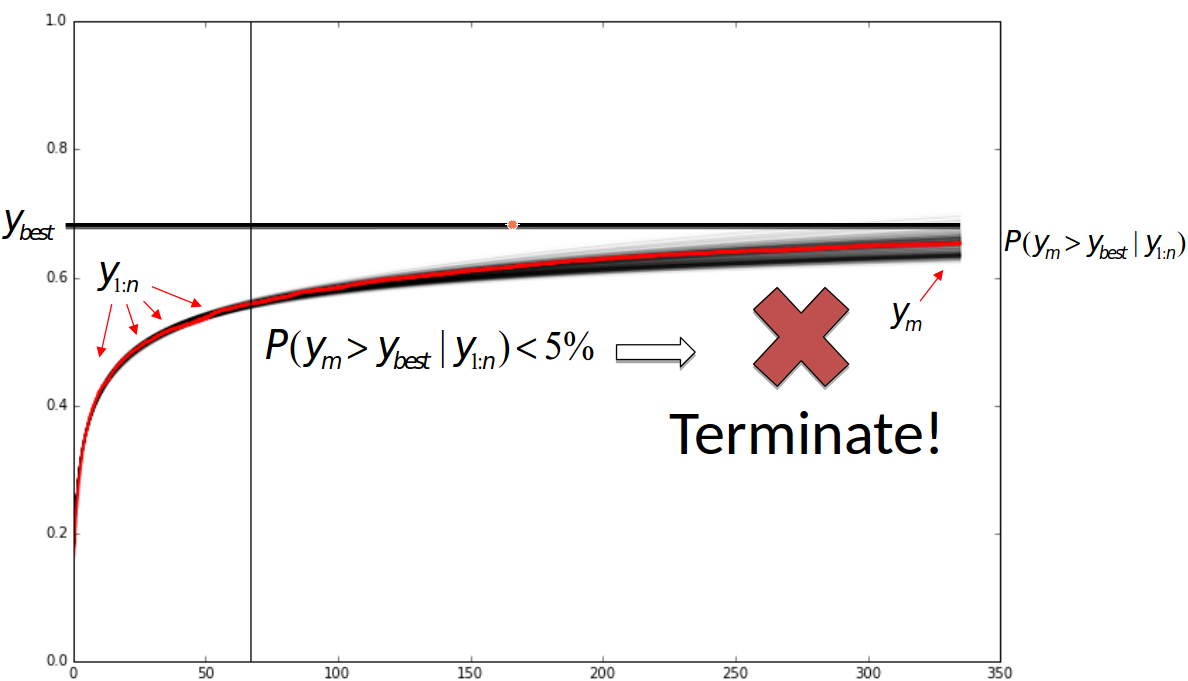
\includegraphics[width=0.8\textwidth]{w07_hpo_grey_box/images/learningcurve/learning_curve_dec2.png}

$\rightarrow$ need for \alert{probabilistic predictions / quantification of uncertainty}

\end{frame}
%-----------------------------------------------------------------------

%-----------------------------------------------------------------------
\begin{frame}{Parametric Learning Curves}

\myit{
	\item Use a parametric model $f_k$ with parameters $\boldsymbol{\theta}$ to model performance at step $t$ as:
	\alert{$y_t = f_k(t|\boldsymbol{\theta}) + \epsilon$}, with $\epsilon \sim \mathcal{N}(0, \sigma^2)$.
\pause
	\item Linear combination of $K=11$ parametric types of models:
	\alert{$f_{comb}(t|\bm{\xi}) = \sum_{k=1}^K w_k f_k(t|\boldsymbol{\theta}_k)$},
where $\bm{\xi} = (w_1, \dots, w_{K}, \boldsymbol{\theta}_1, \dots, \boldsymbol{\theta}_{K}, \sigma^2)$
%	\item MSc Thesis in my group, 2015
}
\begin{center}
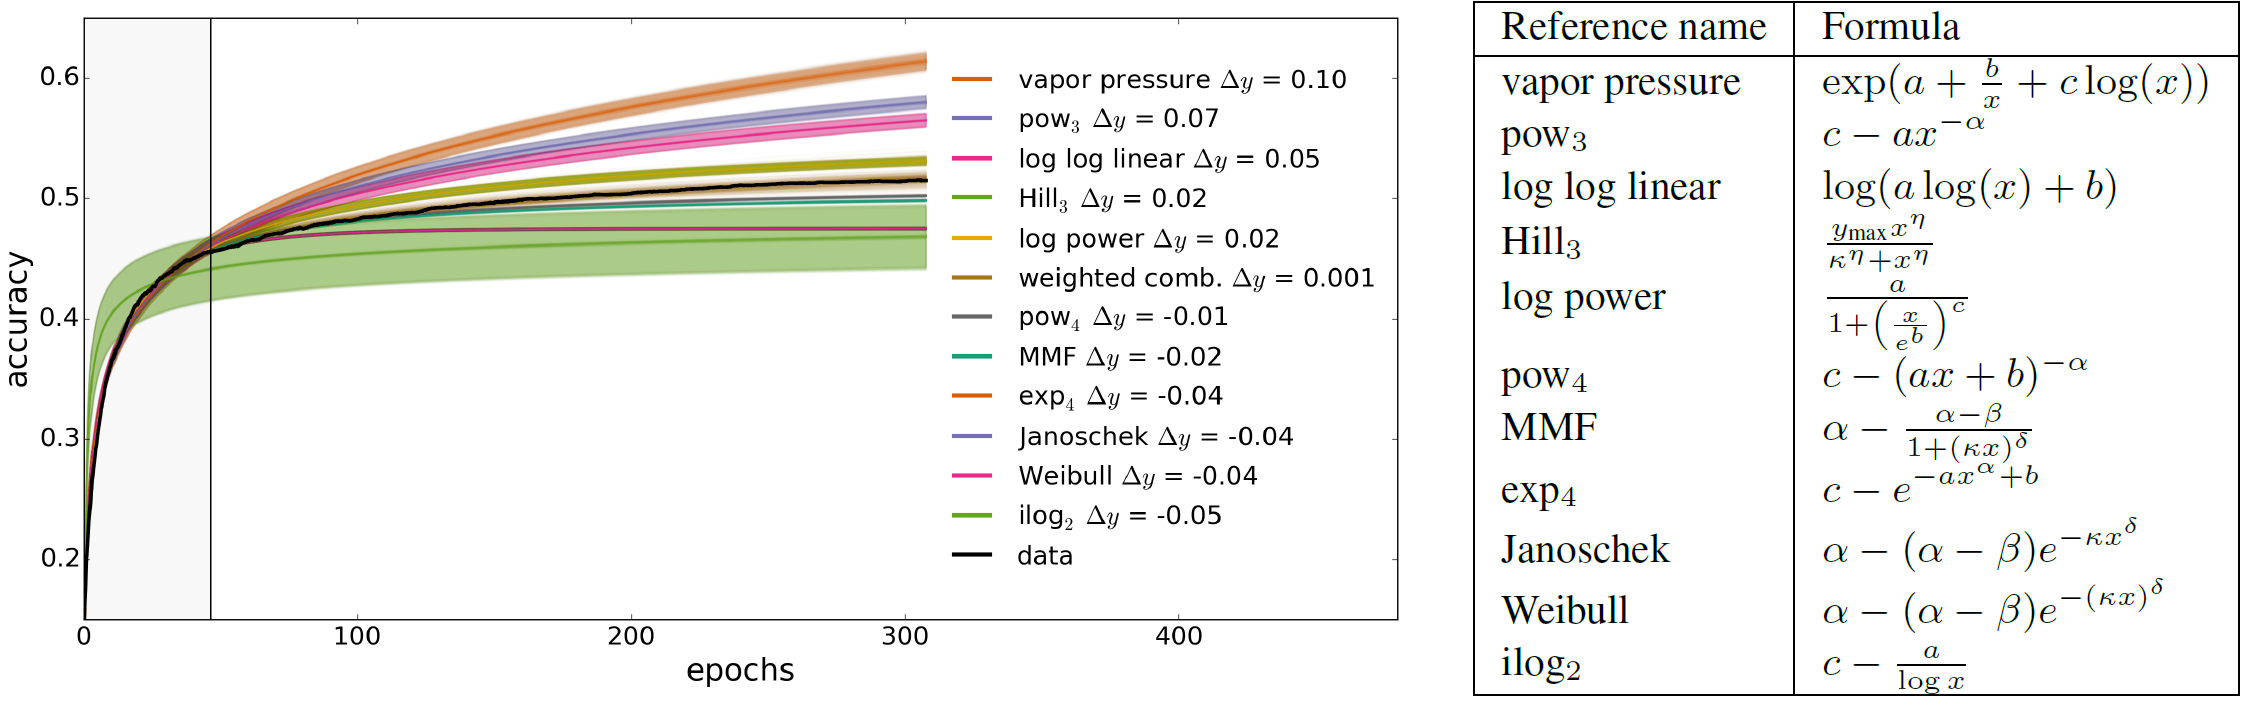
\includegraphics[width=0.9\textwidth]{w07_hpo_grey_box/images/learningcurve/Domhan_types_of_curves.png}\\
\scriptsize{$K=11$ parametric families for modelling learning curves}
\end{center}

\pause
\myit{
	\item Use Markov Chain Monte Carlo sampling of $\bm{\xi}$ to obtain uncertainties
}

\end{frame}
%-----------------------------------------------------------------------

%-----------------------------------------------------------------------
\begin{frame}{Predictive Termination}

{
\begin{center}
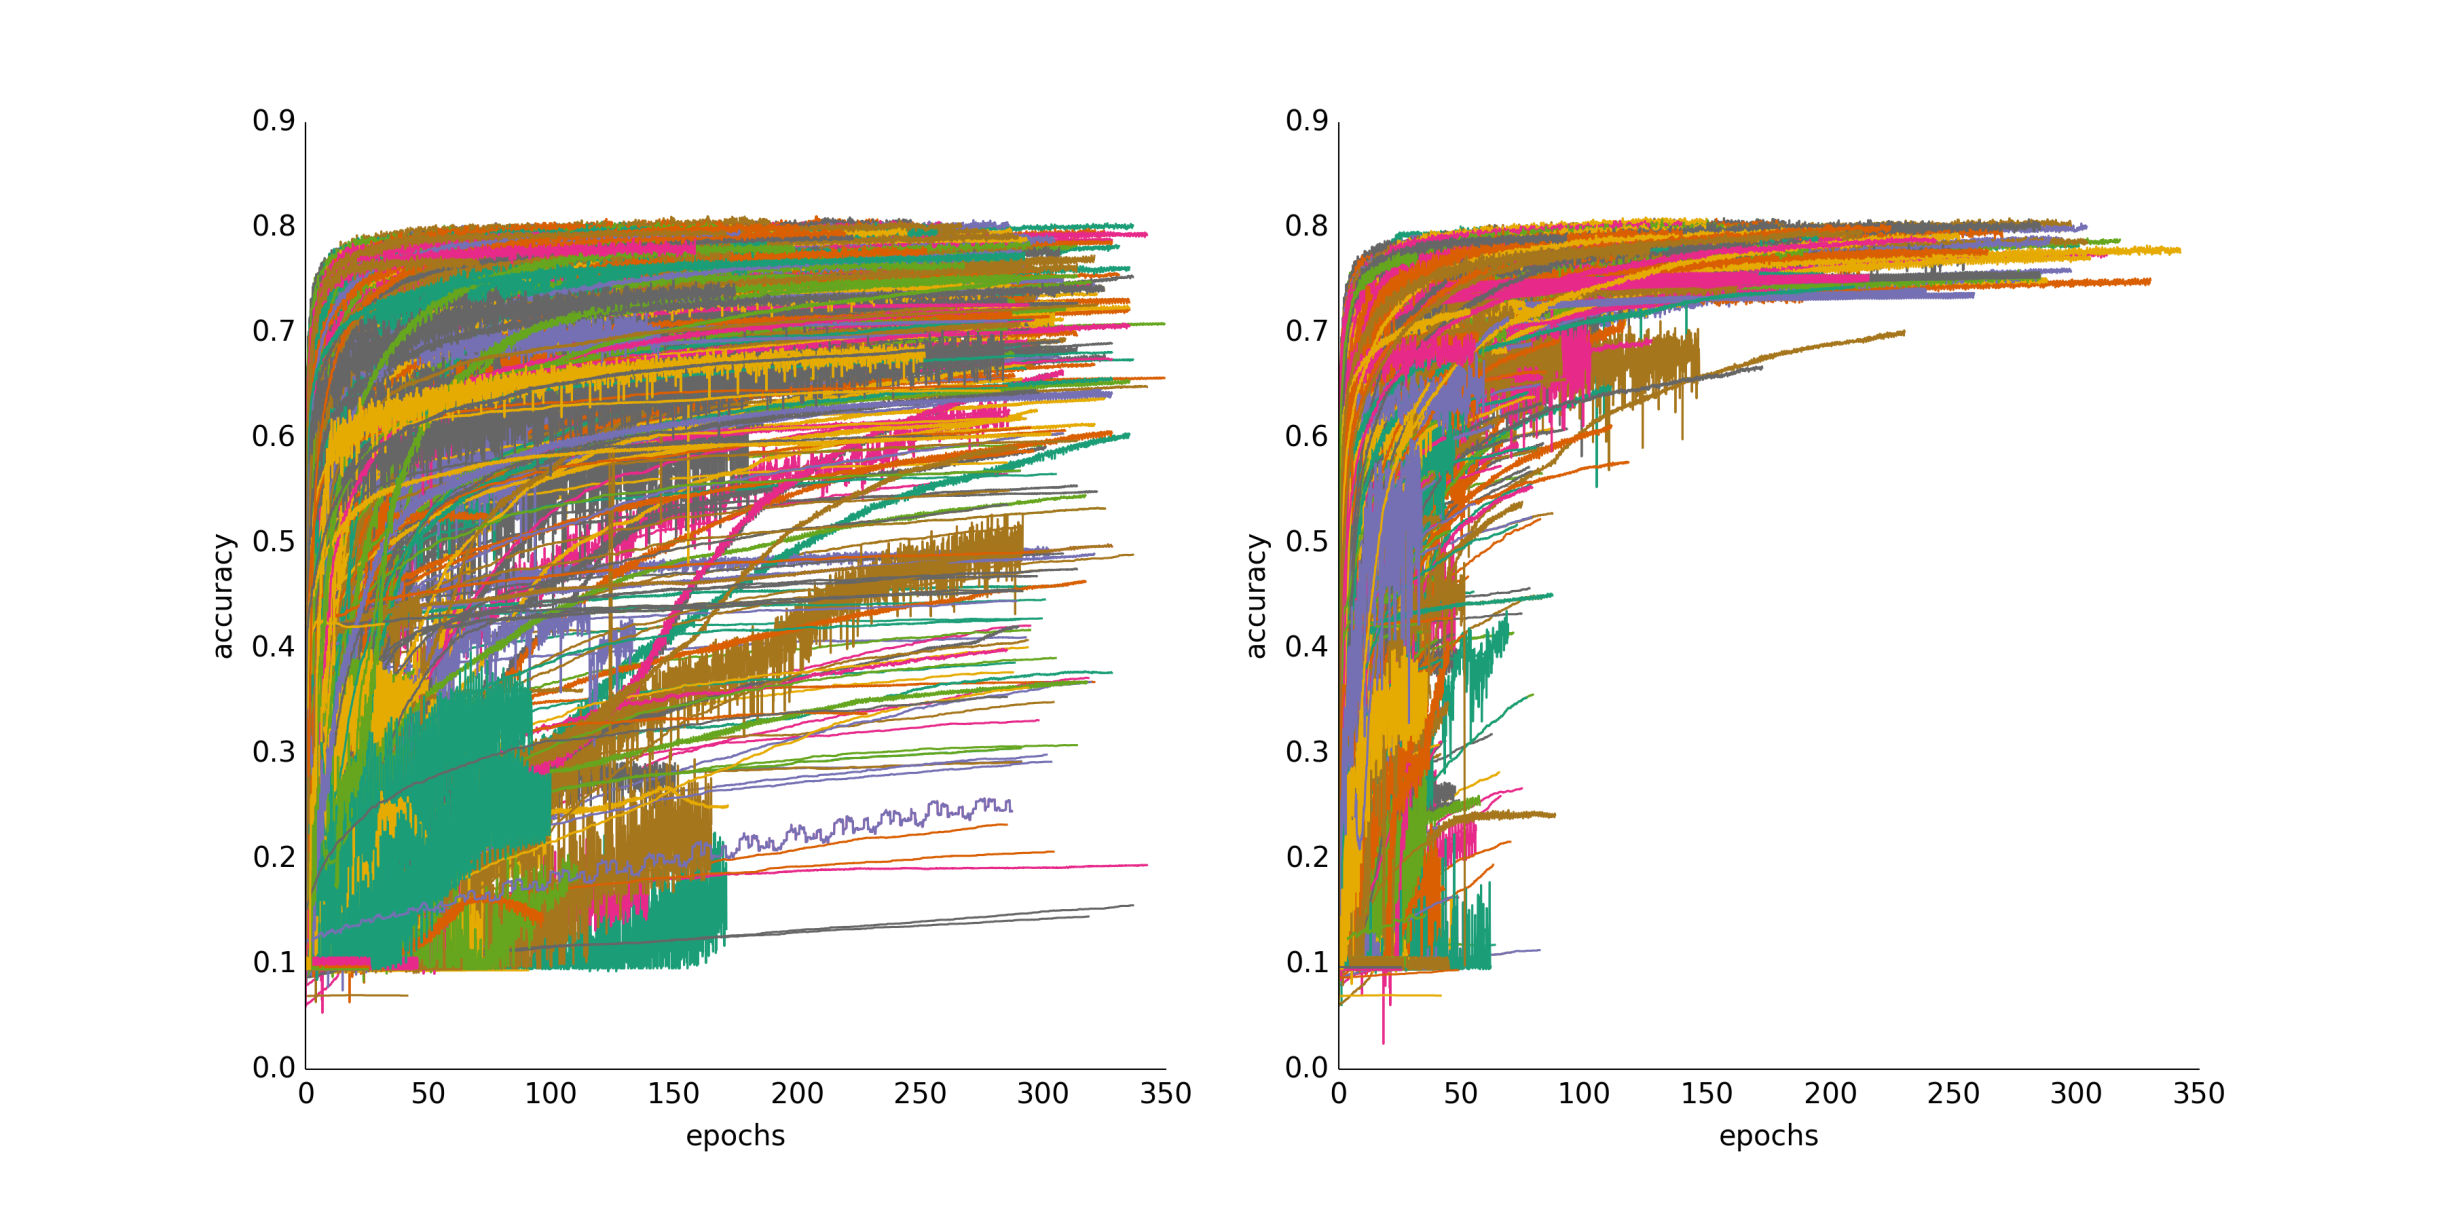
\includegraphics[width=0.9\textwidth]{w07_hpo_grey_box/images/learningcurve/learning_curve_tuning.jpg}

All learning curves vs. learning curves with early termination
\end{center}
}




\end{frame}
%-----------------------------------------------------------------------
%-----------------------------------------------------------------------
\begin{frame}{Predictive Termination}

{
\begin{center}
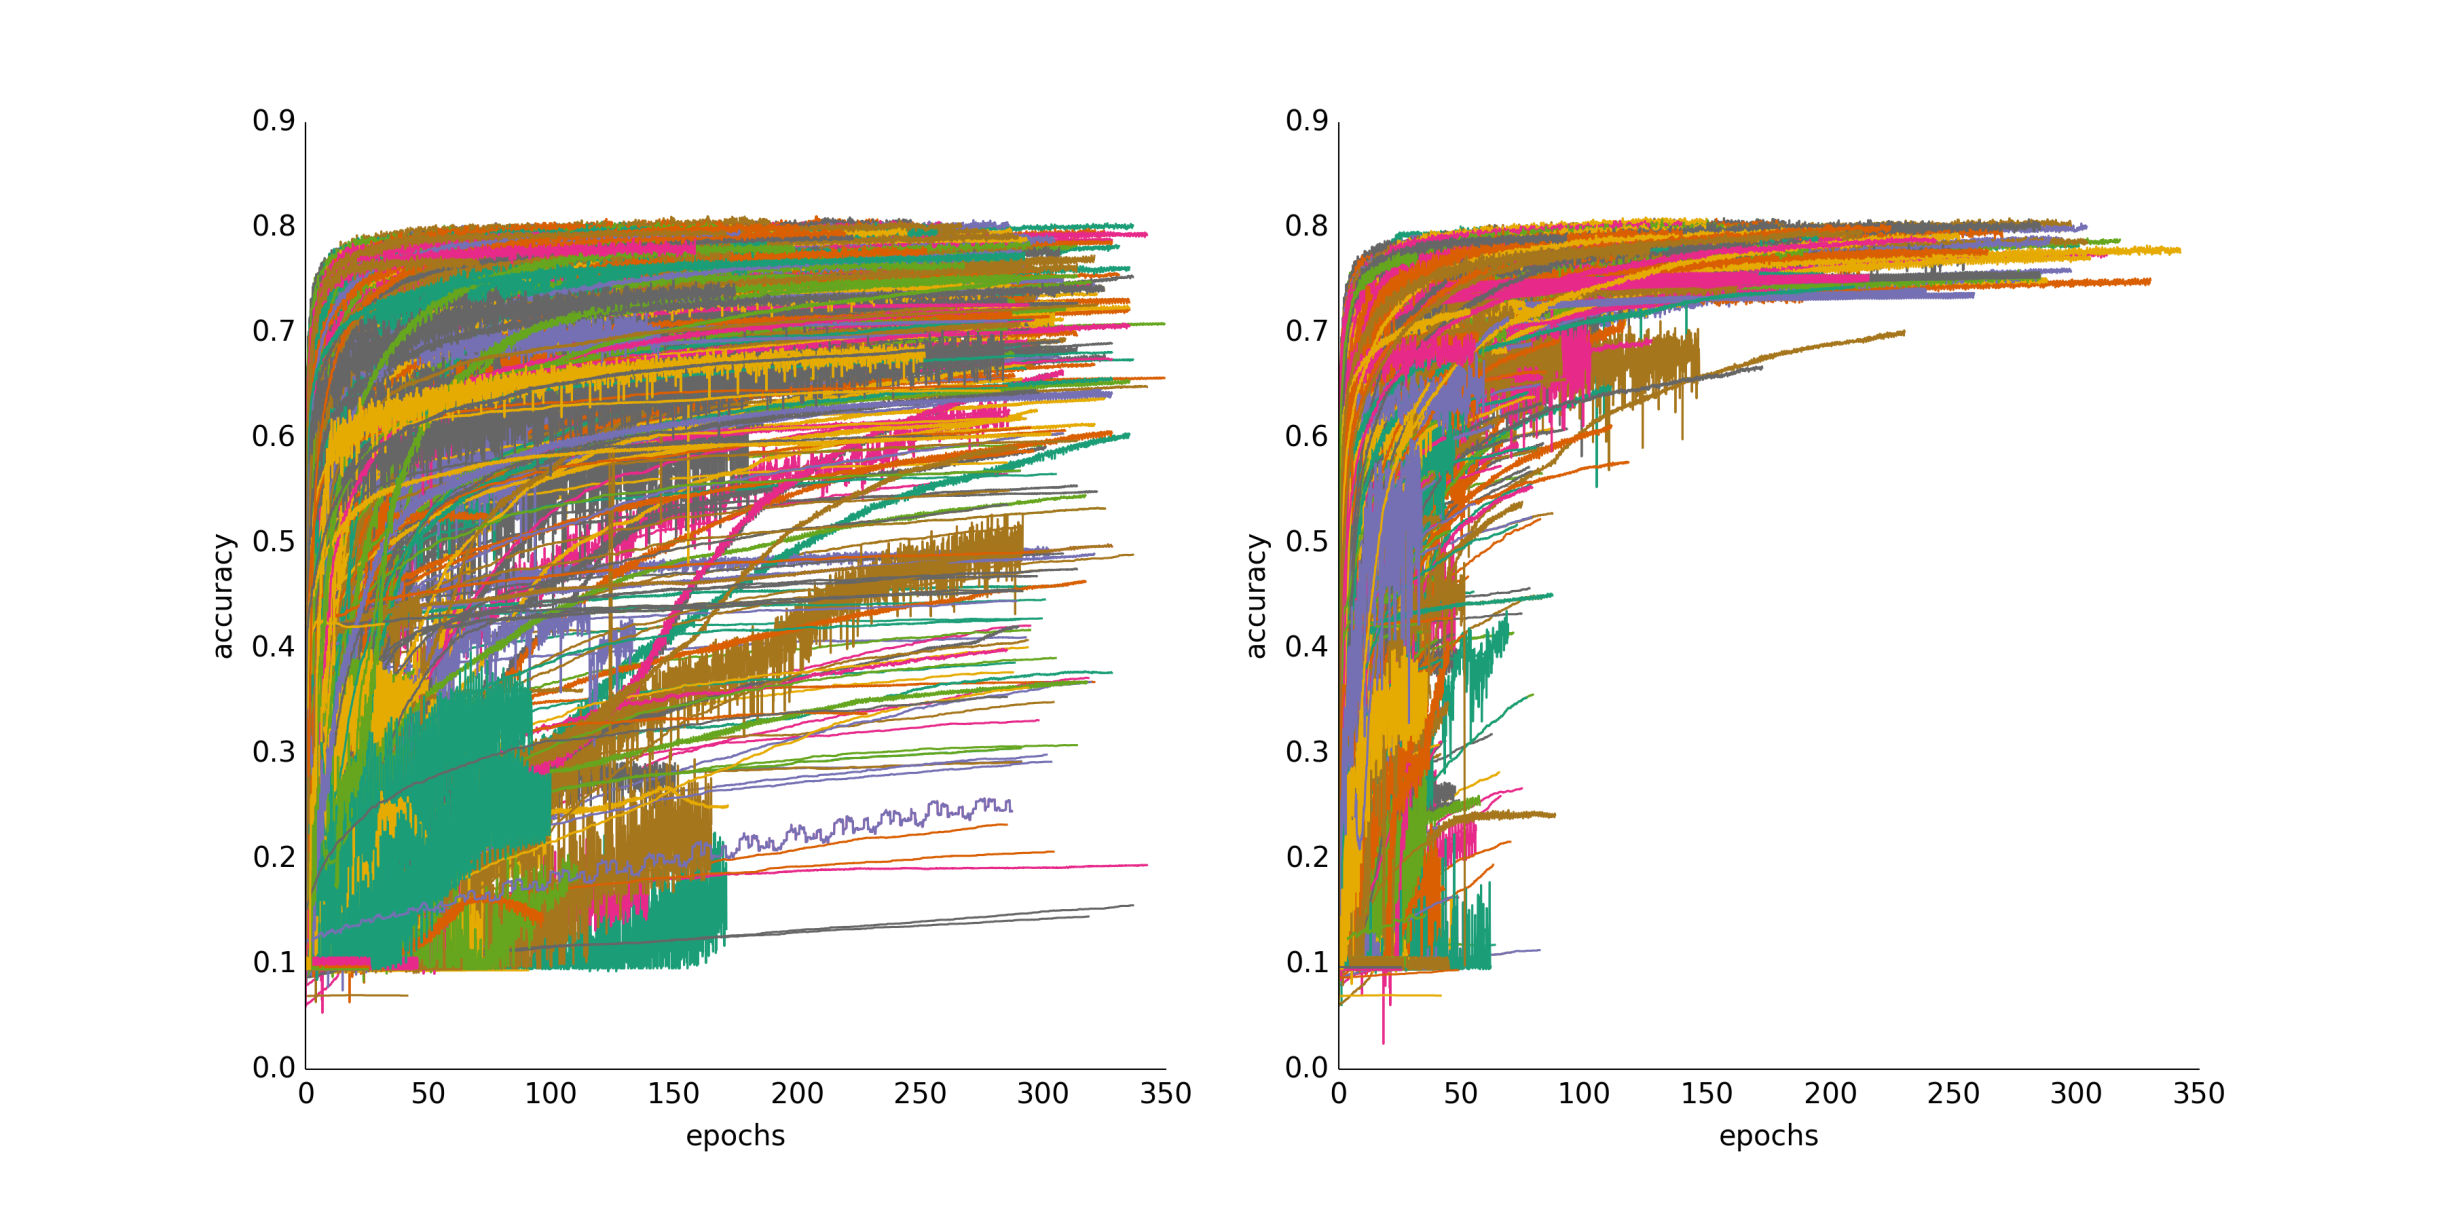
\includegraphics[width=0.5\textwidth]{w07_hpo_grey_box/images/learningcurve/learning_curve_tuning.jpg}

All learning curves vs. learning curves with early termination
\end{center}
}
\myit{
	\item Disadvantages of this model?
\pause
	\myit{
		\item Relies on manually-selected parametric families of curves
		\item Does not take into account hyperparameters used 
		\myit{
			\item[$\rightarrow$] can't learn across hyperparameters
		}
		\item Does not learn across curves; simply extrapolates one at a time
%		\item Cannot quickly integrate new information from extending the curve
	}
}

\end{frame}

%-----------------------------------------------------------------------
\begin{frame}{LC-Net}

\vspace*{-0.25em}
{
	\rightimage[.4]{w07_hpo_grey_box/images/learningcurve/LC-Net-network.png}
	\myit{
		\item \goleft[.45]{Make a layer out of the parametric learning curves by Domhan et al.}
		\item \goleft[.45]{Also support hyperparameters as inputs (in the figure denoted by $x_1, \dots, x_d$)}
%		\item \goleft[.45]{Work by my Phd student Aaron Klein and postdoc Stefan Falkner}
	}
}

\pause
\myit{
	\item Disadvantages of this model?
	\pause
	\myit{
		\item \goleft[.45]{Relies on manually-selected parametric families of curves}
		\item \goleft[.45]{Cannot quickly integrate new information from extending the current curve \\ (or from new runs)}
	}
}
\end{frame}
%-----------------------------------------------------------------------




%-----------------------------------------------------------------------
\begin{frame}{Sequence Models {\smaller{(e.g., Bayesian RNN)}}}

	\myit{
		\item Learning curves are \alert{sequences}
		\myit{
			\item Previous models don't treat them like this
			\item We can use an RNN (in particular, an LSTM) to predict the next value from a given sequence
			\item We can use variational dropout to obtain uncertainty estimates:
\pause
		}
	}

\begin{center}
	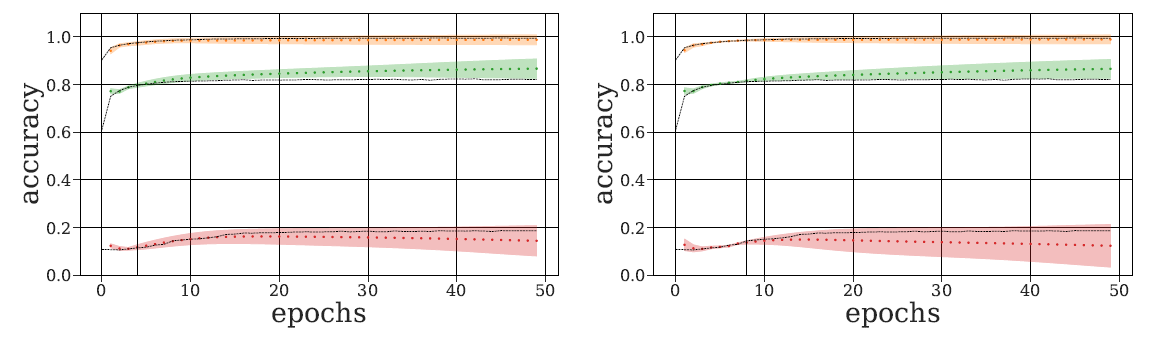
\includegraphics[width=0.58\textwidth]{w07_hpo_grey_box/images/learningcurve/Gargiani-MNIST-extrapolations_1.png}\\
	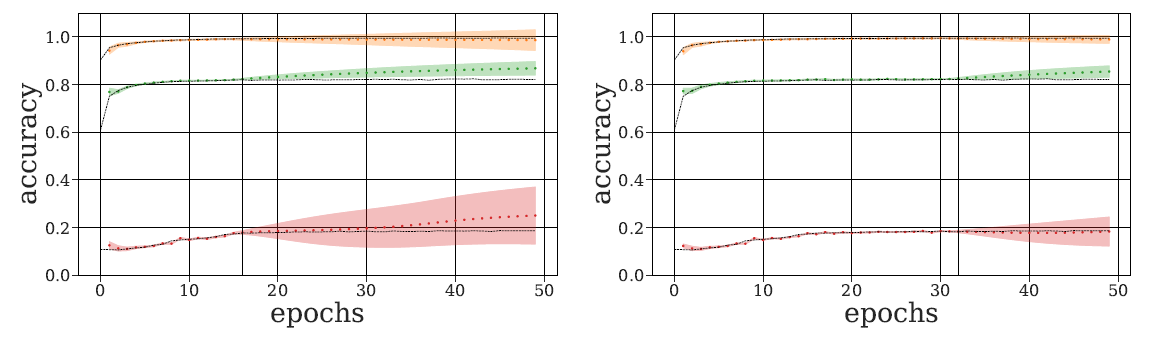
\includegraphics[width=0.58\textwidth]{w07_hpo_grey_box/images/learningcurve/Gargiani-MNIST-extrapolations_2.png}\\
\end{center}	
	
\end{frame}
%-----------------------------------------------------------------------
%-----------------------------------------------------------------------
\begin{frame}{Sequence Models {\smaller{(e.g., Bayesian RNN)}}}

	\myit{
		\item Note: we can also use a simpler model
		\myit{
			\item E.g., a random forest to map from a fixed-size window to the next value
		}
	}
\begin{center}
	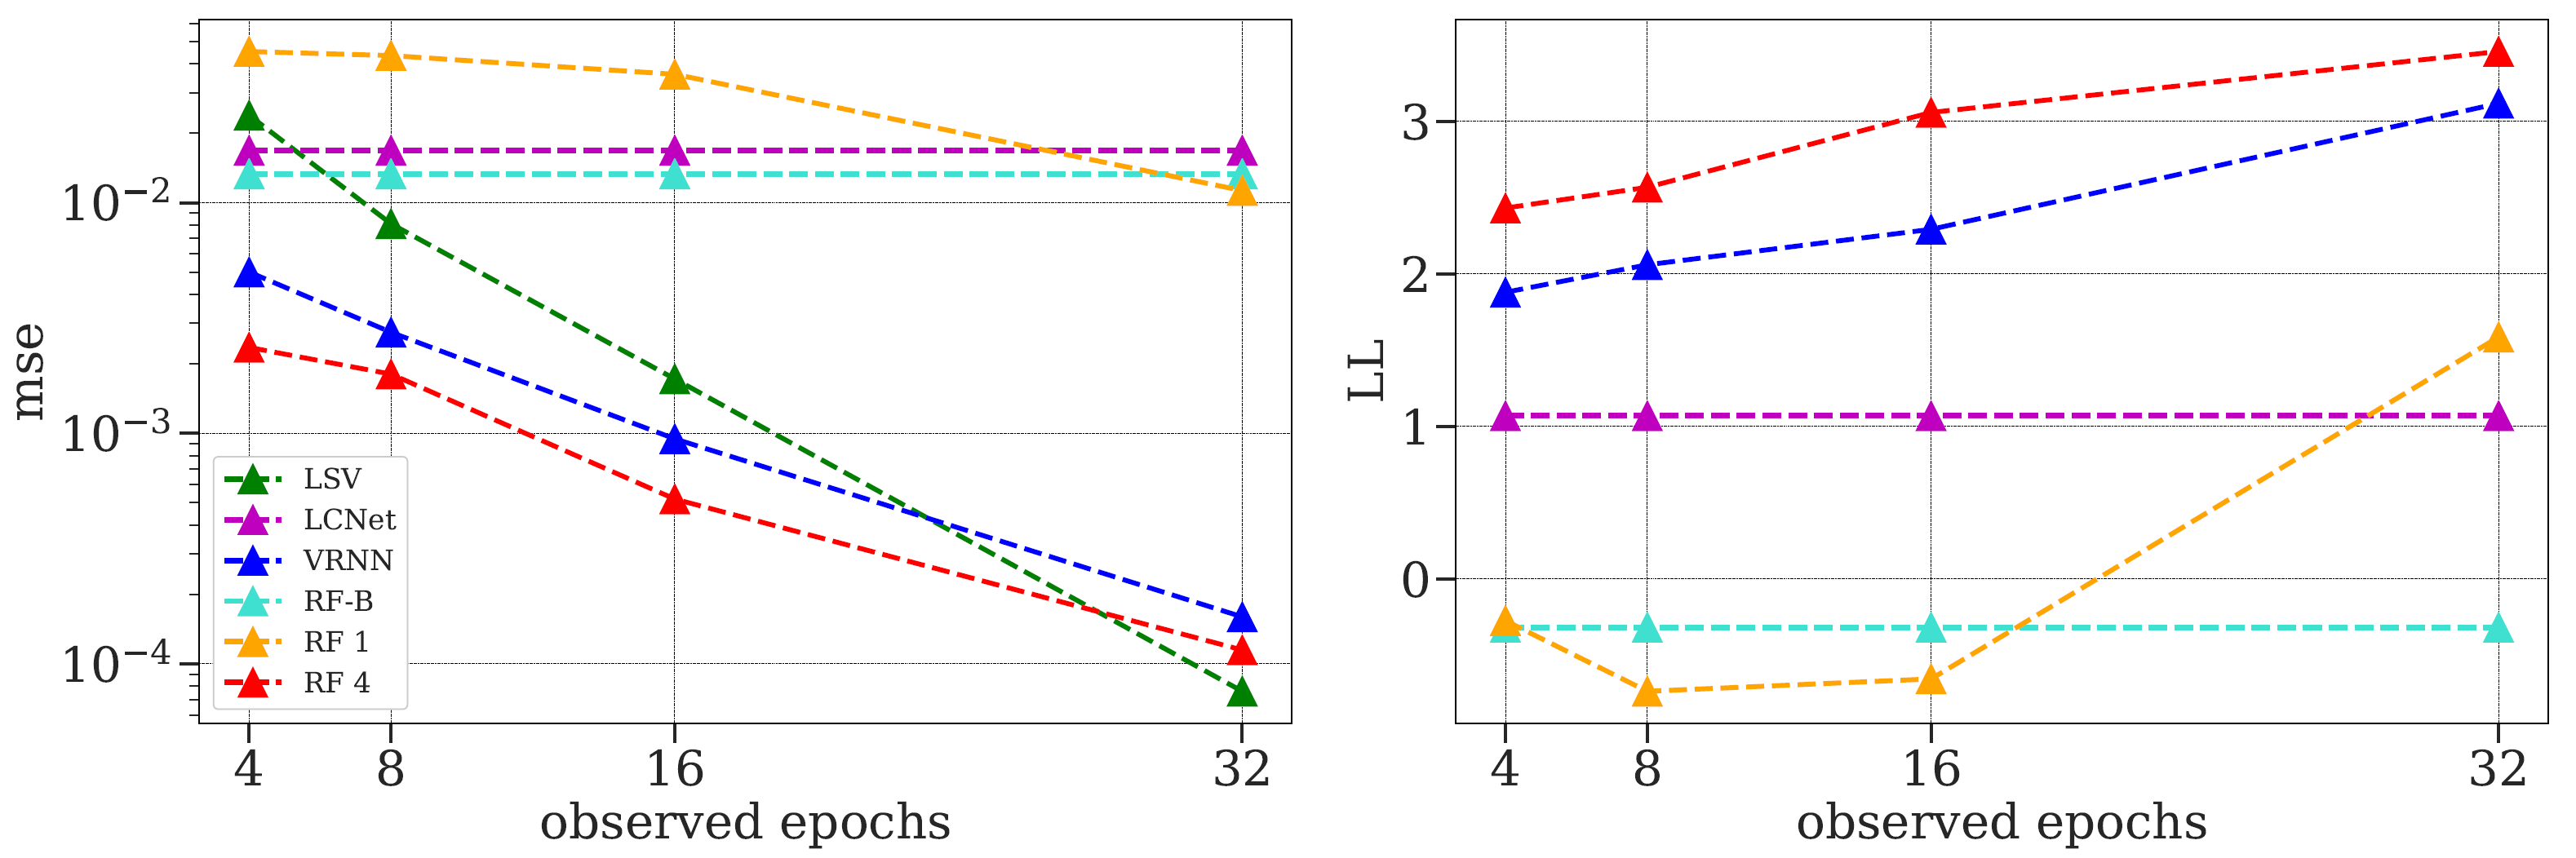
\includegraphics[width=0.9\textwidth]{w07_hpo_grey_box/images/learningcurve/Gargiani-MNIST-extrapolation-quality-based-on-different-sized-prefixes.png}
\end{center}	
\end{frame}
%-----------------------------------------------------------------------
%-----------------------------------------------------------------------
\begin{frame}{Compare: Baker et al, 2017}

	\myit{
		\item Idea: Map from configurations (including architectural hyperparameters) 
		and partial learning curves to the final performance

		\item Advantages
		\myit{
			\item \alert{Much simpler idea} than all the approaches just discussed: no need to model the entire learning curve
			\item \alert{Much easier to implement}
		}
		\item Disadvantage? \pause
		\alert{$\rightarrow$ requires many (e.g., 100) fully-evaluated learning curves as training data}
		\myit{
			\item After 100 full function evaluations we want to be pretty much converged in practice
			\item But definitely helpful for speeding up RL
			
		}
	}

%Describe simple idea, and how that works extremely well when you have a budget of 10.000 of function evaluations.

\end{frame}
%-----------------------------------------------------------------------
%-----------------------------------------------------------------------
\begin{frame}{Freeze-Thaw Bayesian Optimization}

\myit{
	\item Use a Gaussian process with inputs $\conf$ and $t$; special kernel for $t$
	\item For $N$ configurations and $T$ epochs each: $O(N^3 t^3)$ $\rightarrow$ approximation
	\item Iteratively: either extend existing configuration or try new one
\pause
	\item Result for probabilistic matrix factorization:
	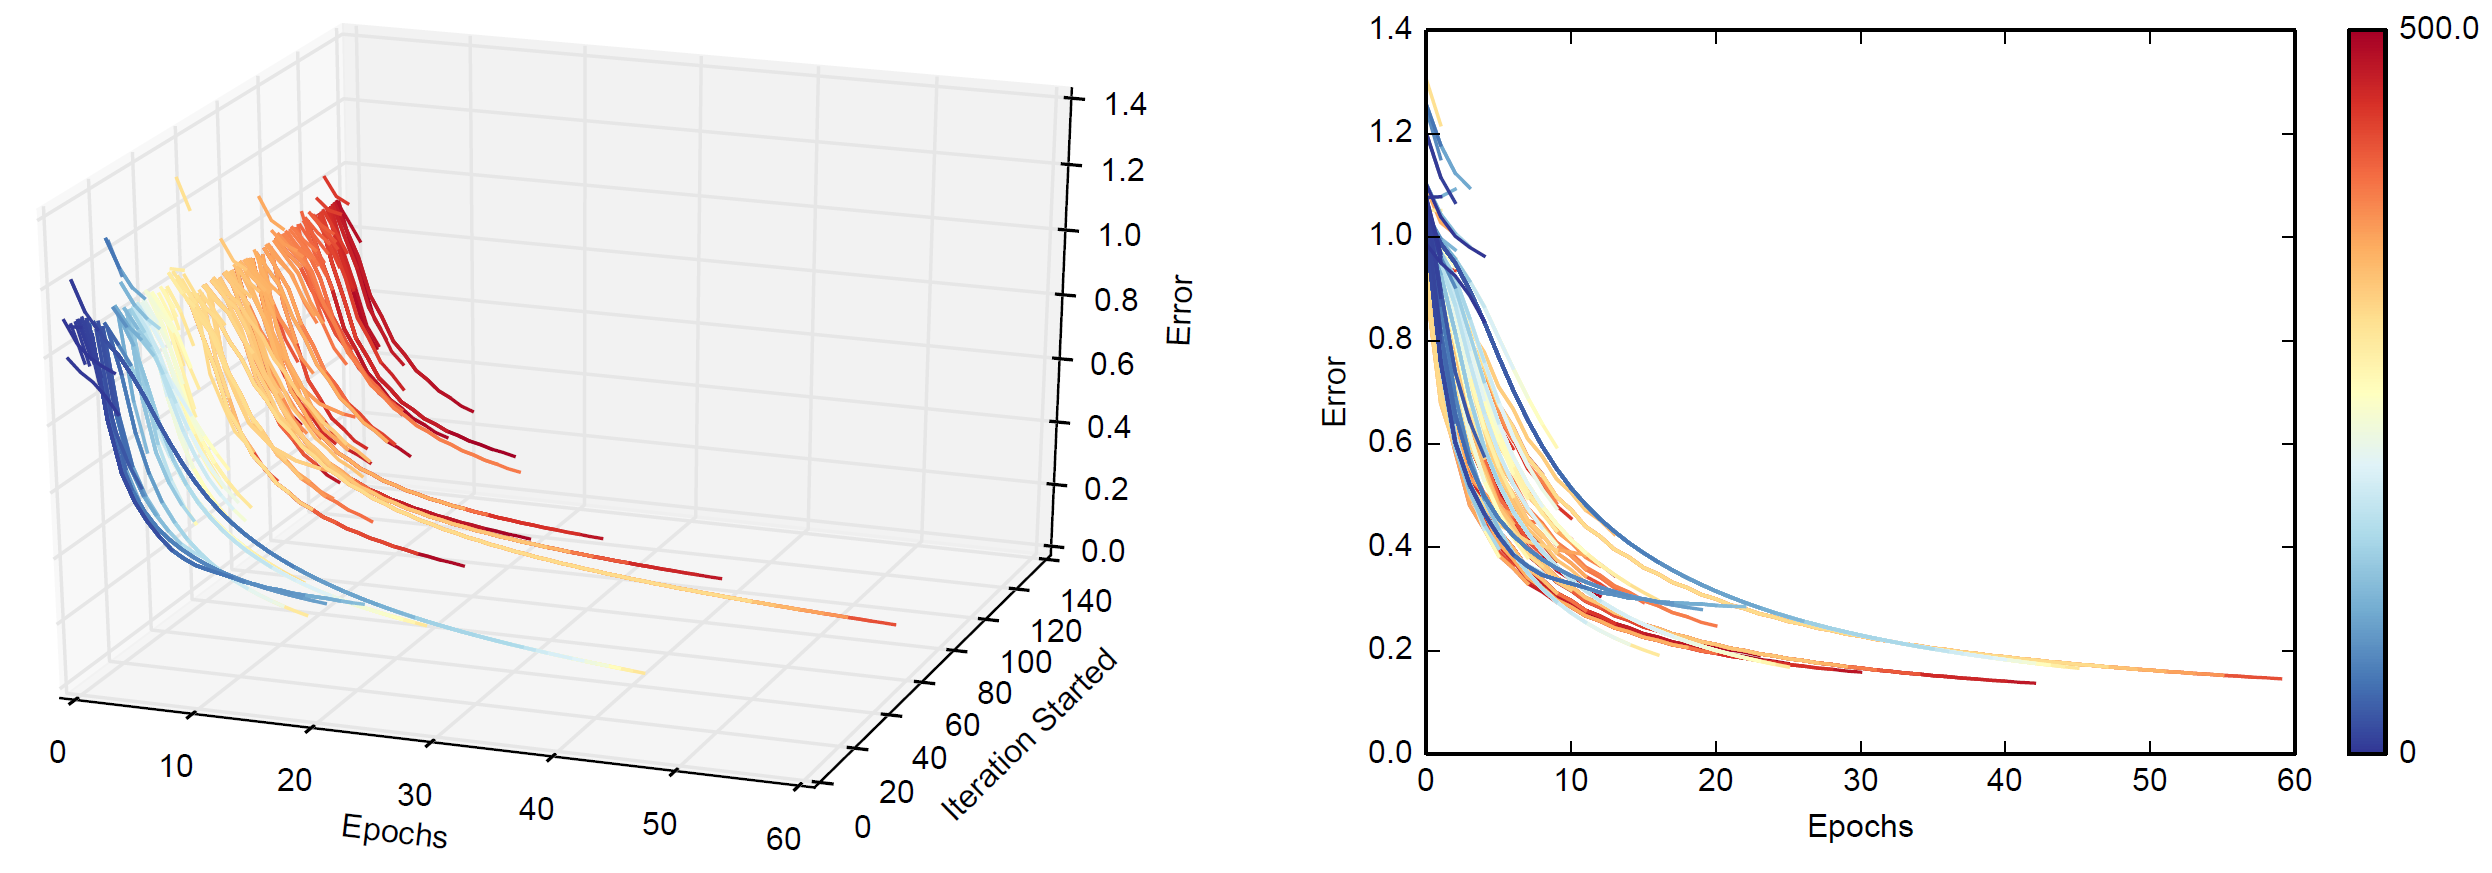
\includegraphics[width=0.8\textwidth]{w07_hpo_grey_box/images/learningcurve/FTBO.png}
\pause
	\item Unfortunately, no results for DNNs; no code available
}


\end{frame}
%-----------------------------------------------------------------------




\myframe{Possible extension of LC models waiting to be done}{
	\myit{
		\item We could keep track of additional information to feed to our model for better predictions
		\myit{
			\item E.g., training \& validation cross-entropy loss \& accuracy
			\myit{
				\item Instead of only validation accuracy
			}
			\item E.g., split cross-entropy into data-dependent \& weight dependent parts
			\item E.g., keep track of gradient norms, activation statistics, \ldots
		}
\bigskip
        \item Information about learning rate (\& weight decay) at each step
%		\begin{itemize}
%		    \item Only Predictive termination leads to a practically usable algorithm
%		\end{itemize}
	}
}

%-----------------------------------------------------------------------
\begin{frame}[c]{Questions to Answer for Yourself / Discuss with Friends}

\begin{itemize}
    \item 
    \alert{Discussion.} 
    \begin{itemize}
        \item Is it dangerous (in terms of performance) to cut evaluations early on, i.e., could one cut evaluations that would be final best?
        \item How would you set the new hyperparameters, such as the 5\% for early learning curve termination, in practice?
    \end{itemize}
\end{itemize}

\end{frame}
%\section{Overview of Multi-Fidelity Optimization}
%----------------------------------------------------------------------
\begin{frame}[c]{Motivating Example}

\begin{itemize}
    \item Performance of a support vector machine (SVM) on MNIST and subsets of it:\\~\\
	    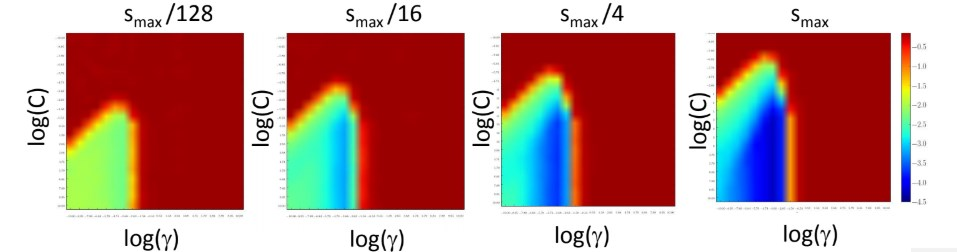
\includegraphics[width=0.9\textwidth]{../w07_hpo_speedup/images/fabolas/example_mnist.jpg}
	    \begin{itemize}
            \item Computational cost grows quadratically in dataset size $z$
            \item Error shrinks smoothly with $z$
        \end{itemize}
\bigskip
    \item Evaluations on the smallest subset (about 400 data points) cost 10\,000$\times$ less than on the full data set (50\,000 data points)
    
\end{itemize}
\end{frame}
%----------------------------------------------------------------------

%----------------------------------------------------------------------
\begin{frame}[c]{Motivating Example 2: Shorter Runs of Anytime Algorithms}

\begin{itemize}
    \item Performance with shorter runs of an anytime algorithm (such as SGD):\\~\\
\centering
\includegraphics[width=0.5\linewidth]{../w07_hpo_speedup/images/hyperband/Figure_1_2.png}

\end{itemize}
\end{frame}
%----------------------------------------------------------------------


%----------------------------------------------------------------------
\myframe{Multi-Fidelity Optimization In General}{

Exploit cheap approximations of an expensive blackbox function $\rightarrow$ afford more configurations\\

\begin{columns}[T]
    \begin{column}{.5\textwidth}
        \myit{
            \item Idea: eliminate poor configurations early, allocate more resources to promising ones.
        }
    \end{column}
    
    \begin{column}{.4\linewidth}
        \begin{figure}
        \centering
        \includegraphics[width=0.9\linewidth]{../w07_hpo_speedup/images/hyperband/Figure_1_2.png}
        \end{figure}
    \end{column}
\end{columns}

\begin{columns}
    \begin{column}{.9\linewidth}
    \vspace{-10em}
\pause
\medskip
    \myit{
    	\item Possible Resources:
    	\myit{
    	    \item Runtime
    	    \item Number of epochs/iterations
    	    \item Data subset size
    	    \item Downsampled size of images in object recognition
    	    \item Depth / width of neural networks
    	    \item Number of trees 
    	    \item Number of features
    	    \item Number of cross validation folds\\~
    	    \item General concept, even in fields outside ML, e.g., fluid simulation:
    	    \myit{
    	        \item Number of particles
    	        \item Time scale of simulation
    	    }
    	}
    }
\end{column}
\begin{column}{0\linewidth}
\end{column}
\end{columns}
}


%----------------------------------------------------------------------
\begin{frame}[c]{General Remarks on Multi-Fidelity Optimization}

\myit{
    \item Often, we have a \alert{choice} which resources we use as budget
\bigskip
\pause
    \item For multi-fidelity optimization to be helpful, \alert{performance with low budgets should be informative about performance with high budgets}  
\bigskip    
\pause  
    \item In the simplest case: 
    Good with low resources $\leftrightarrow$ good with high resources.
    \myit{
        \item In practice, this is of course not always true
    }
    
}


\end{frame}



%-----------------------------------------------------------------------
\begin{frame}{How Useful is the Cheap Approximation? The Rank Correlation}

Given:
\myit{
    \item A set of configurations $\pcs = \{\conf_1, ..., \conf_n\}$
    \item The performances $f(\conf_1), ..., f(\conf_n)$ on the expensive black box
    \item The performances $g(\conf_1), ..., g(\conf_n)$ on a cheap approximation of the black box

\bigskip
\pause

}
    We compute the \alert{Spearman rank correlation} between $[f(\conf_1), ..., f(\conf_n)]$ and $[g(\conf_1), ..., g(\conf_n)]$
\myit{    
    \item If this is high (in the extreme: 1), the relative ranking of the configurations is the same on $f$ and $g$
    \myit{
        \item In that case, we can optimize cheaply on $g$ and also obtain an optimum for $f$
    }
    \item If it is low, optimizing g does not tell us anything about f

}

\bigskip
\pause
Goal: find approximations g that are very cheap but have high rank correlations with f

\end{frame}
%----------------------------------------------------------------------

%-----------------------------------------------------------------------
\begin{frame}{Questions to Answer for Yourself / Discuss with Friends}

\bigskip

\begin{itemize}
    \item \alert{Repetition.} Which cheap approximation is better in this hypothetical case?
    \myit{
        \item Downscaling images (5x cheaper, rank correlation of 0.8)
        \item Less epoch of SGD (4x cheaper, rank correlation of 0.75)
    }

\medskip
    \item \alert{Discussion.} 
    Can you think of a multi-fidelity approximation we did not discuss yet?

\end{itemize}

\end{frame}
%----------------------------------------------------------------------
%----------------------------------------------------------------------
%\section{Multi-fidelity Bayesian optimization}
%----------------------------------------------------------------------
%----------------------------------------------------------------------
\begin{frame}[c]{Motivating example}

\begin{itemize}
    % \item Traditional Bayesian hyperparamter optimizers model \\ the loss of ML algorithm given the dataset and seek to find \\ the minimum of such black-box function.
    % \item \emph{FABOLAS} models the loss and computational cost \\ \alert{across dataset size} and carries BO with an extra degree of freedom.
    \item Performance of an SVM on MNIST and subsets of it:\\~\\
	    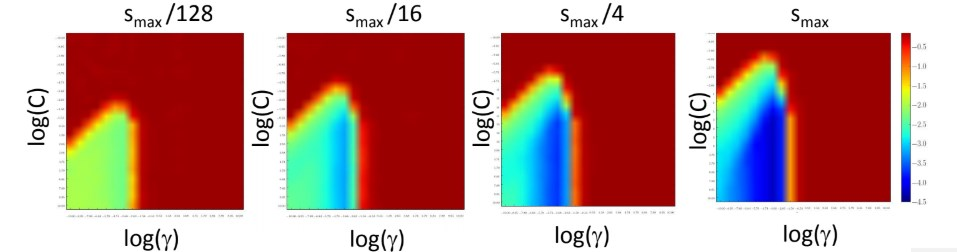
\includegraphics[width=0.9\textwidth]{../w07_hpo_speedup/images/fabolas/example_mnist.jpg}
	    \begin{itemize}
            \item Computational cost grows quadratically in dataset size $z$
            \item Error shrinks smoothly with $z$
        \end{itemize}
	\item Evaluations on the smallest subset (about 400 data points) cost 10\,000$\times$ less than on the full data set
    
\end{itemize}
\end{frame}
%----------------------------------------------------------------------
%----------------------------------------------------------------------

%----------------------------------------------------------------------
%----------------------------------------------------------------------
\begin{frame}[c]{Idea}

\alert{Multi-fidelity Bayesian optimization} for fidelity with values $z\in \mathcal{Z}$ 
\begin{itemize}
	\item Standard Bayesian optimization uses a model $\surro(\conf) \approx y$ to select the next $\conf$
	\item \alert{Multi-fidelity} Bayesian optimization uses a model $\surro(\conf\alert{, z}) \approx y$ to select the next $(\conf\alert{, z})$
    \pause
    \bigskip
    

	
%	\item BOCA - a general approach
%	\begin{itemize}
%	    \item Introduces continuity in fidelity space
%		\item Based on \alert{UCB}
%	\end{itemize}
%   
%	\item FABOLAS - a Gaussian process for extrapolating from small to large datasets
%	\begin{itemize}
%		\item This approach uses dataset size as a fidelity $(z \in [0, 1])$
%		\item Based on \alert{Entropy Search}
%	\end{itemize}


    \item Our goal:
        \begin{equation*}
            \optconf = \argmin_{\conf \in \pcs} \func(\conf) = \argmin_{\conf \in \pcs} \surro(\alert{z_{\bullet}}, \conf)
        \end{equation*}

    \pause
    \bigskip

    \item Model $\surro$ needs to be good at extrapolating from small to large $z$

\end{itemize}




\end{frame}
%----------------------------------------------------------------------
%----------------------------------------------------------------------

%----------------------------------------------------------------------
%----------------------------------------------------------------------
%\begin{frame}[c]{Bayesian Optimization with Continuous Approximations}
%
%\begin{itemize}
%    \item \emph{Goal.} Use the cheap approximations to guide search for the optimum of $\func$, \\ reduce the overall cost of optimization
%    \item \emph{Example.} Tuning of a classification algorithm over a space of hyperparameters $\conf$ 
%        \begin{itemize}
%            \item using $N_{\bullet}$ data points
%            \item via iterative algorithm for $T_{\bullet}$ iterations
%        \end{itemize}
%    \item \emph{Solution.} Approximate validation loss using fewer data points $N < N_{\bullet}$ and/or fewer iterations $T < T_{\bullet}$, such that search deploys:
%        \begin{itemize}
%            \item cheap low fidelity experiments with small $(N, T)$ to discard bad hyperparameters 
%            \item expensive high fidelity experiments with large $(N, T)$ for promising regions
%        \end{itemize}
%    
%\end{itemize}
%\end{frame}
%----------------------------------------------------------------------
%----------------------------------------------------------------------

%----------------------------------------------------------------------
%----------------------------------------------------------------------
%\begin{frame}[c]{Bayesian Optimization with Continuous Approximations}
%
%\begin{itemize}
%
%        \begin{itemize}
%            \item surrogate function $\surro : \alert{\mathcal{Z}} \times \conf \rightarrow  \mathbb{R}$
%            \item e.g. fidelity space $\mathcal{Z} = [1, N_{\bullet}] \times  [1, T_{\bullet}], z_{\bullet} = [N_{\bullet}, T_{\bullet}]$
%
%        \end{itemize}
%
%    \item Determine the fidelity $\iter[\bocount]{z} \in \mathcal{Z}$ to query $\surro$:
%        \begin{enumerate}
%            \item Select a subset  $\iter[\bocount]{Z}$ of $\mathcal{Z}$, that:
%                \begin{itemize}
%                    \item considers only cheaper fidelities,
%                    \item trades of \emph{information gain} and \emph{cost} while enforcing more exploration \\ in cheaper regions in the early stage of the search, %
%                    \item excludes fidelities in a close neighborhood of $z_{\bullet}$.
%                \end{itemize}
%            \item If the subset is empty: $\iter[\bocount]{z} = z_{\bullet}$
%            \item Otherwise: $\iter[\bocount]{z} \in \argmin_{z \in \iter[\bocount]{Z}} \cost(z)$
%        \end{enumerate}
%
%\end{itemize}
%\end{frame}
%----------------------------------------------------------------------
%----------------------------------------------------------------------

% %----------------------------------------------------------------------
% %----------------------------------------------------------------------
% \begin{frame}[c]{Fast Bayesian Optimization on Large Datasets}
% \framesubtitle{Multi-fidelity Bayesian optimization}

% \alert{Multi-fidelity Bayesian optimization} for fidelity with values $z\in \mathcal{Z}$ 
% \begin{itemize}
% 	\item Standard Bayesian optimization uses a model $\func(\conf) \approx y$ to select the next $\conf$
% 	\item \alert{Multi-fidelity Bayesian optimization} uses a model $\func(\conf\alert{, z}) \approx y$ to select the next $(\conf\alert{, z})$
%     \pause
%     \smallskip
    
% 	\item Model $\func$ needs to be good at extrapolating from small to large $z$
	
% 	\item E.g., a Gaussian process for extrapolating from small to large datasets - FABOLAS
% 	\begin{itemize}
% 		\item This approach uses dataset size as a fidelity $(z \in [0, 1])$,
% 		\item based on \alert{Entropy Search},
% 		\item achieved 1\,000-fold speedups for SVM on MNIST example.
% 	\end{itemize}
% \end{itemize}
% \end{frame}
% %----------------------------------------------------------------------
% %----------------------------------------------------------------------

%----------------------------------------------------------------------
%----------------------------------------------------------------------
\begin{frame}[c]{Entropy Search - reminder}

\begin{itemize}
		\item Define the $p_{\text{min}}$ distribution given data $\dataset$:
		$$p_{\text{min}}(\conf^* \mid \alert{\dataset}) := p(\conf^* \in \argmin_{\conf\in \pcs} \func(\conf) \mid \alert{\dataset})$$
	
		\item Entropy search aims to minimize the entropy \alert{$\mathcal{H}[p_\text{min}]$} 
		\item In a nutshell:
		\begin{enumerate}
			\item Estimate $p(\func \mid \dataset)$, e.g., using a GP (as before)
			\item Approximate $p_\text{min}$ by representer points and Monte-Carlo simulations
			\item Select $\conf$ that minimizes the following acquisition function:
		\end{enumerate}
\end{itemize}
\vspace*{0.5cm}
	\[{\acq}_{ES}(\conf) := \mathds{E}_{\alert{p(\tilde{\cost}\mid \conf, \dataset)}} 
	\left[   \mathcal{H}[p_{\text{min}}(\cdot \mid \alert{\dataset \cup \left\langle \conf, \tilde{\cost} \right\rangle })] \right]\]

\end{frame}
%----------------------------------------------------------------------
%----------------------------------------------------------------------

%----------------------------------------------------------------------
%----------------------------------------------------------------------
\begin{frame}[c]{Fast Bayesian Optimization on Large Datasets: Overview}

\begin{itemize}
		\item We care about the $p_{\text{min}}$ distribution for the maximal budget $z_{\bullet}$:
		$$p_{\text{min}}(\conf^* \mid \dataset) := p(\conf^* \in \argmin_{\conf\in \pcs} \func(\conf\alert{,z_{\bullet}}) \mid \dataset)$$
	
		\item We still want to minimize the entropy $\mathcal{H}[p_\text{min}]$
\pause
		\item Now we aim for the biggest \alert{reduction in entropy per time spent}
		\begin{itemize}
			\item Now we don't model only $\func$, but also \alert{the cost $c(\conf,z)$}
			\item We choose the next $(\conf,z)$ by maximizing:
		\end{itemize}
\end{itemize}
\vspace*{0.5cm}
	\[{\acq}_{ES}(\conf,\dataset) := \mathds{E}_{\alert{p(\tilde{\cost}\mid (\conf, z), \dataset)}} 
	\left[   \frac{\mathcal{H}[p_{\text{min}}(\cdot \mid \alert{\dataset})] - \mathcal{H}[p_{\text{min}}(\cdot \mid \alert{\dataset \cup \left\langle (\conf,z), \tilde{\cost} \right\rangle}}{\alert{c(\conf,z)}} \right]\]

\end{frame}
%----------------------------------------------------------------------
%----------------------------------------------------------------------

%----------------------------------------------------------------------
%----------------------------------------------------------------------
\begin{frame}[c]{Fast Bayesian Optimization on Large Datasets: Overview}

\begin{itemize}
    \item The entire algorithm iterates the following 2 steps until time is up:
		\begin{enumerate}
			\item Select $(\conf,s)$ by maximizing:
    			\[{\acq}_{ES}(\conf,\dataset) := \mathds{E}_{\alert{p(\tilde{\cost}\mid (\conf, z), \dataset)}} 
            	\left[   \frac{\mathcal{H}[p_{\text{min}}(\cdot \mid \alert{\dataset})] - \mathcal{H}[p_{\text{min}}(\cdot \mid \alert{\dataset \cup \left\langle (\conf,z), \tilde{\cost} \right\rangle}}{\alert{c(\conf,z)}} \right]\]
			\item Observe performance and cost, and update models $\func$ and $\cost$ 
		\end{enumerate}

\pause

\begin{columns}[T] % align columns
\begin{column}{.48\textwidth}


    \begin{block}{Advantages}
    \begin{itemize}
    	\item Conceptually beautiful
    	\item 1\,000-fold speedups for optimizing SVMs on MNIST
    \end{itemize}
    \end{block}
\pause
\end{column}%

\hfill%

\begin{column}{.48\textwidth}

    \begin{block}{Disadvantages}
    \begin{itemize}
    	\item \alert{Scalability} of GPs is a big problem (limits size of initial design)
    	\item Limited applicability of Gaussian processes
    \end{itemize}
\end{block}

\end{column}
\end{columns}   

\end{itemize}
\end{frame}
%----------------------------------------------------------------------
%----------------------------------------------------------------------


% %----------------------------------------------------------------------
% %----------------------------------------------------------------------
% \begin{frame}[c]{Fast Bayesian Optimization on Large Datasets}
% \framesubtitle{Overview}

% \begin{itemize}
%     \item Automatically choose dataset size for each evaluation
%         \begin{itemize}
%             \item Include extra dimension in probabilistic model to capture \\ dependence on dataset size $s$: $\func(\conf, s)$
%             \item Construct a second model for computational cost: $\cost(\conf, s)$
%             \item Trade off information gain about global optimum vs. cost
%         \end{itemize}
%     \item Extend the GP by an additional input dimension: $s \in [0, 1]$
%         \begin{itemize}
%             \item standard stationary kernel (over HPs) + covariance function in $s$
%                 \begin{equation*}
%                     \kernel( (\conf, s), (\conf', s') ) = \kernel_{5/2} (\conf, \conf') ( \phi^{T}(s) * \Sigma_{\phi} * \phi(s') )
%                 \end{equation*}
%             \item  we use the same form of kernel to model the loss $\func$ and cost $\cost$, but with different basis functions $\phi_{\func}$ and $\phi_{\cost}$
%                 \begin{itemize}
%                     \item $\phi_{\func}(s) = (1, (1-s)^2)^T$
%                     \item $\phi_{\cost}(s) = (1, s)^T$
%                 \end{itemize}
%         \end{itemize}
        
% \end{itemize}

% \source{Klein, Bartels, Falkner, Hennig, Hutter, AISTATS 2017}
% \end{frame}
% %----------------------------------------------------------------------
% %----------------------------------------------------------------------

%----------------------------------------------------------------------
%----------------------------------------------------------------------
\begin{frame}[c]{Fast Bayesian Optimization on Large Datasets: Results}

\centering
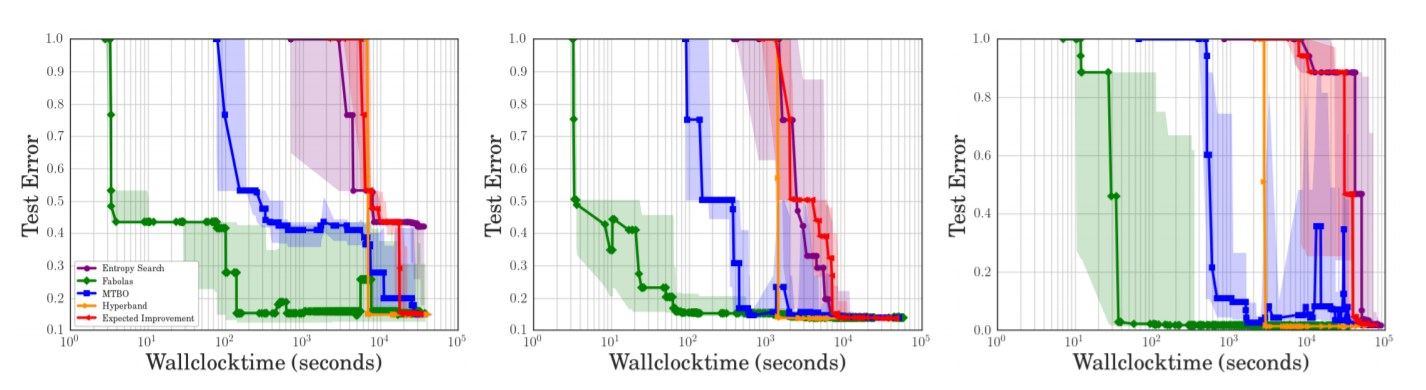
\includegraphics[width=1.\textwidth]{../w07_hpo_speedup/images/fabolas/fabolas_results.jpg}

\hspace{12cm}{\lit{\href{http://proceedings.mlr.press/v54/klein17a/klein17a.pdf}{Klein et al. 2017}}}
\end{frame}
%----------------------------------------------------------------------
%----------------------------------------------------------------------


\begin{frame}{Questions to Answer for Yourself / Discuss with Friends}

\bigskip

\begin{itemize}
    \item \alert{Discussion.} 
    \begin{itemize}
        \item What kind of cost model should be incorporated into the FABOLAS algorithm?
        \item Could one use other acquisition functions than entropy search for FABOLAS?
    \end{itemize}
    

\end{itemize}

\end{frame}
%%----------------------------------------------------------------------
\section{Hyperband}

%-----------------------------------------------------------------------

% \begin{frame}{Bandit-Based Hyperparameter Optimization}
% \begin{columns}[T]

% \begin{column}{.45\textwidth}
%     \begin{itemize}
%         \item Idea: Allocate more resources to promising configurations, eliminate poor ones early.
%         \pause
%     \end{itemize}
% \end{column}
%     \begin{column}{.45\linewidth}
%     \begin{figure}
%     \centering
%     \includegraphics[width=0.9\linewidth]{w07_hpo_grey_box/images/hyperband/Figure_1_2.png}
% \end{figure}
%     \end{column}
%     \end{columns}
%     \begin{columns}
    
%     \begin{column}{.45\linewidth}
%     \vspace{-9em}
%     \begin{itemize}
% 	\item Result: Examine more configurations.
% 	\pause
% 	\item Resources:
% 	\pause
% 	\begin{itemize}
% 	    \item Runtime
% 	    \pause
% 	    \item Number of epochs/iterations
% 	    \pause
% 	    \item Number of trees
% 	    \pause
% 	    \item Data subset size
% 	    \pause
% 	    \item Number of features
% 	    \pause
% 	    \item Number of cross validation folds
	    
% 	    \item ...
% 	\end{itemize}
% \end{itemize}
% \end{column}

% \begin{column}{.45\textwidth}

% \end{column}

% \end{columns}

% \end{frame}

% %-----------------------------------------------------------------------

% \begin{frame}{Successive Halving(SH)}
% \begin{columns}

% \begin{column}{.45\textwidth}
% \vspace{-1em}
% \begin{itemize}
%     \item Simple technique
%     \item Assumes promising configurations outperform bad configurations, even early on in the algorithm run.
%     %\item Bandit-based approach to hyperparameter optimization.
%     \pause
%     \item Uniformly allocate a budget to a set of configurations.
%     \pause
% \end{itemize}
% \end{column}

% \begin{column}{.5\textwidth}
% \begin{figure}
%     \centering
%     \vspace{3em}
%     \only<3>{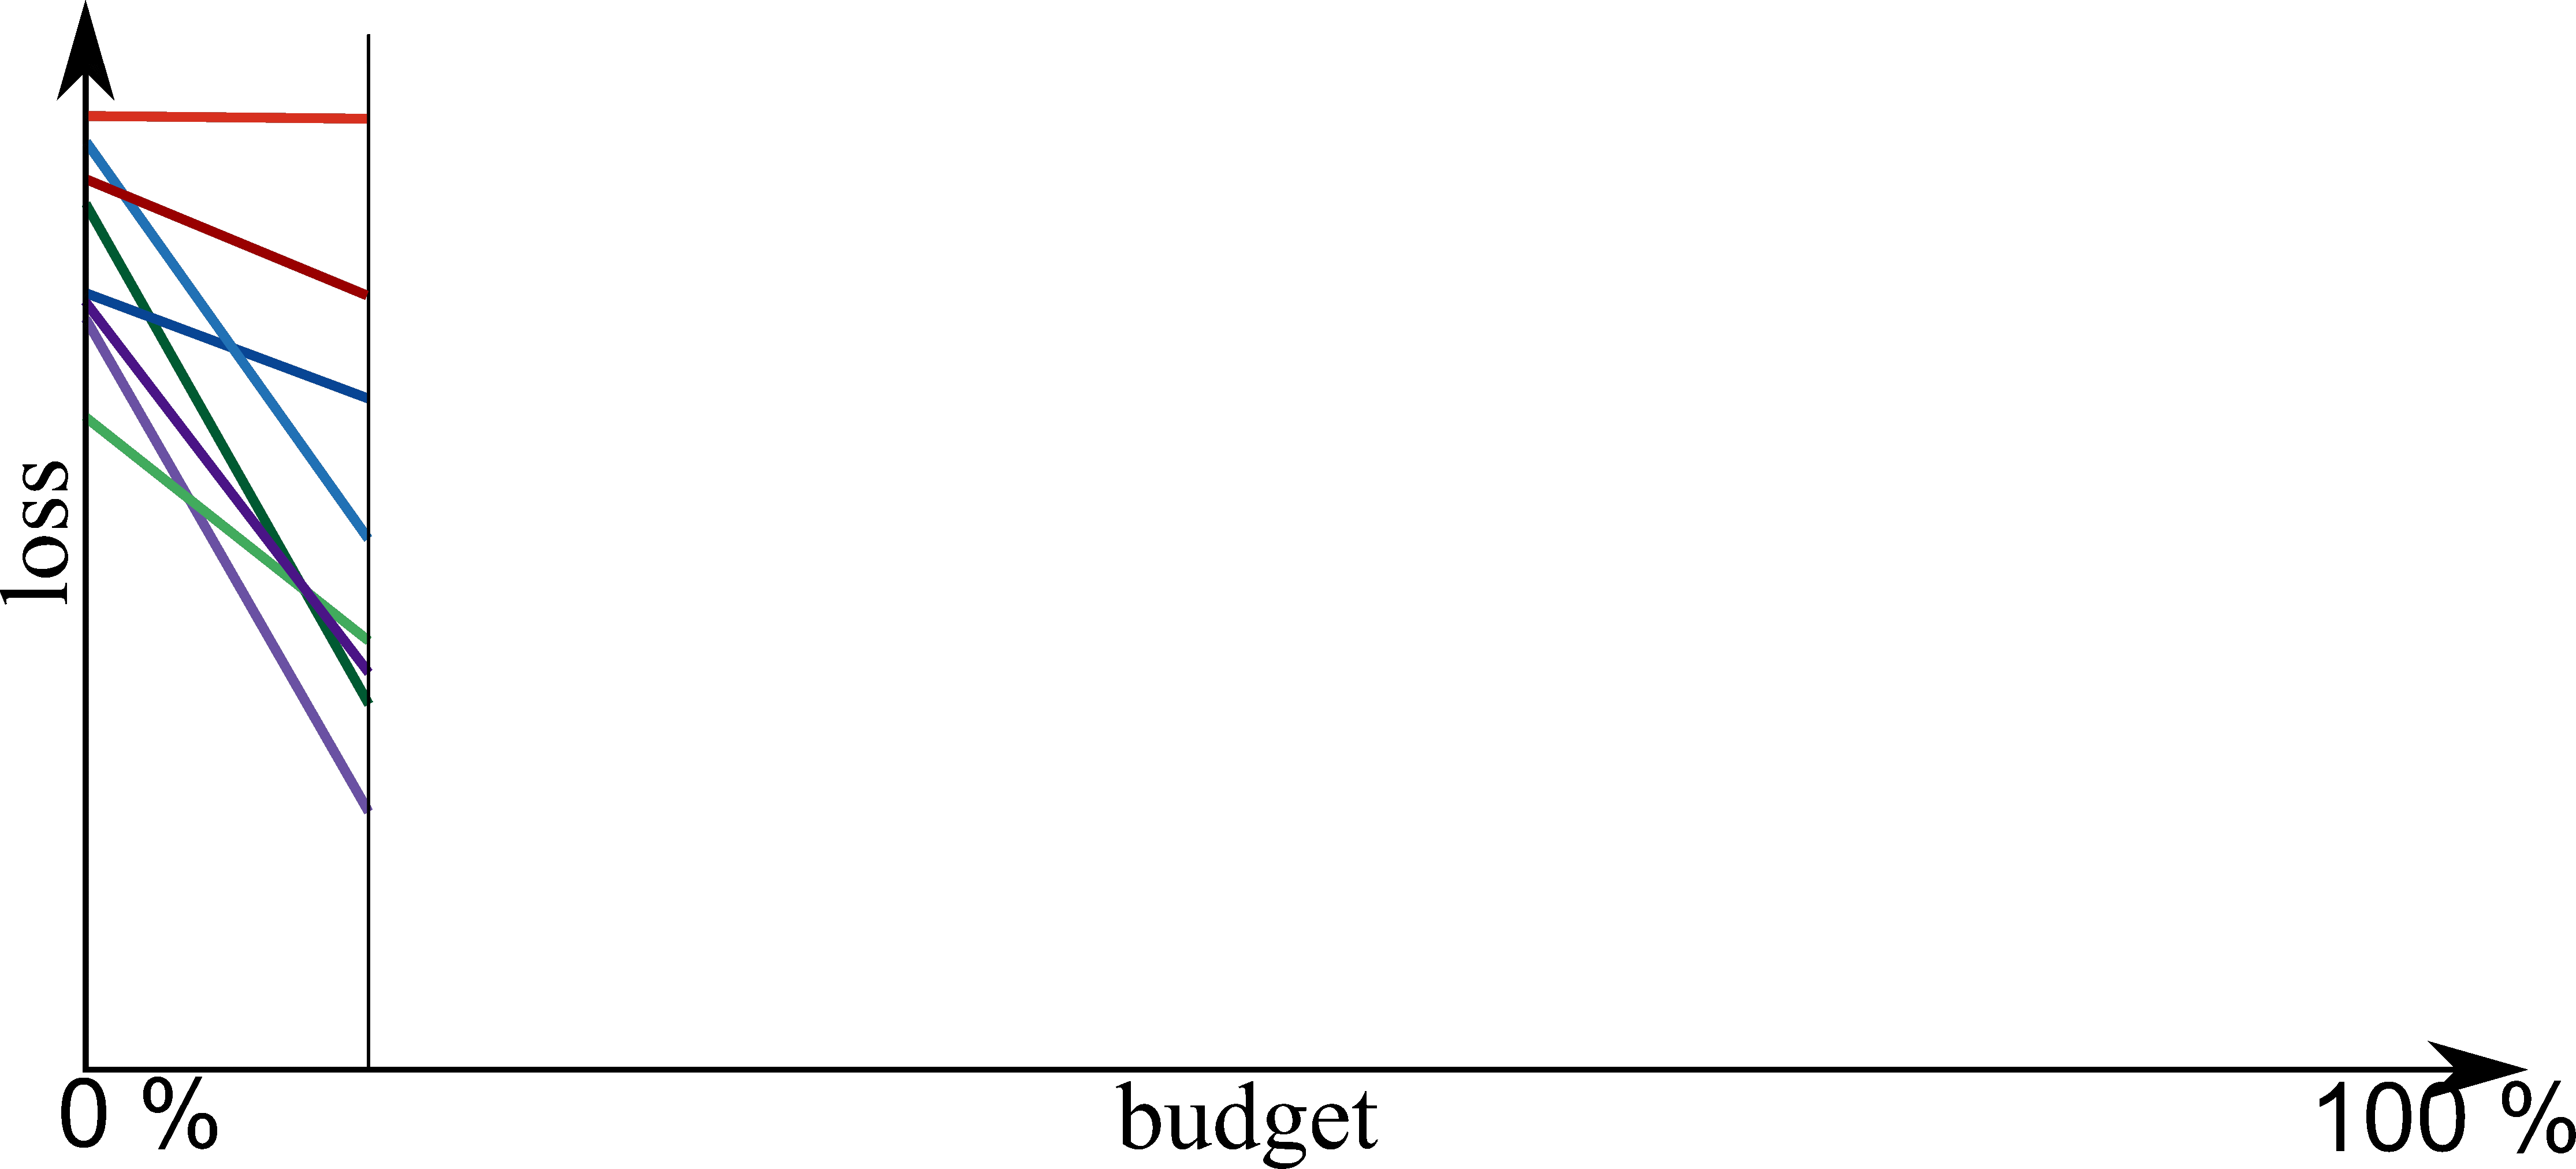
\includegraphics[width=\linewidth]{w07_hpo_grey_box/images/hyperband/SH-1.png}}
%     \only<4>{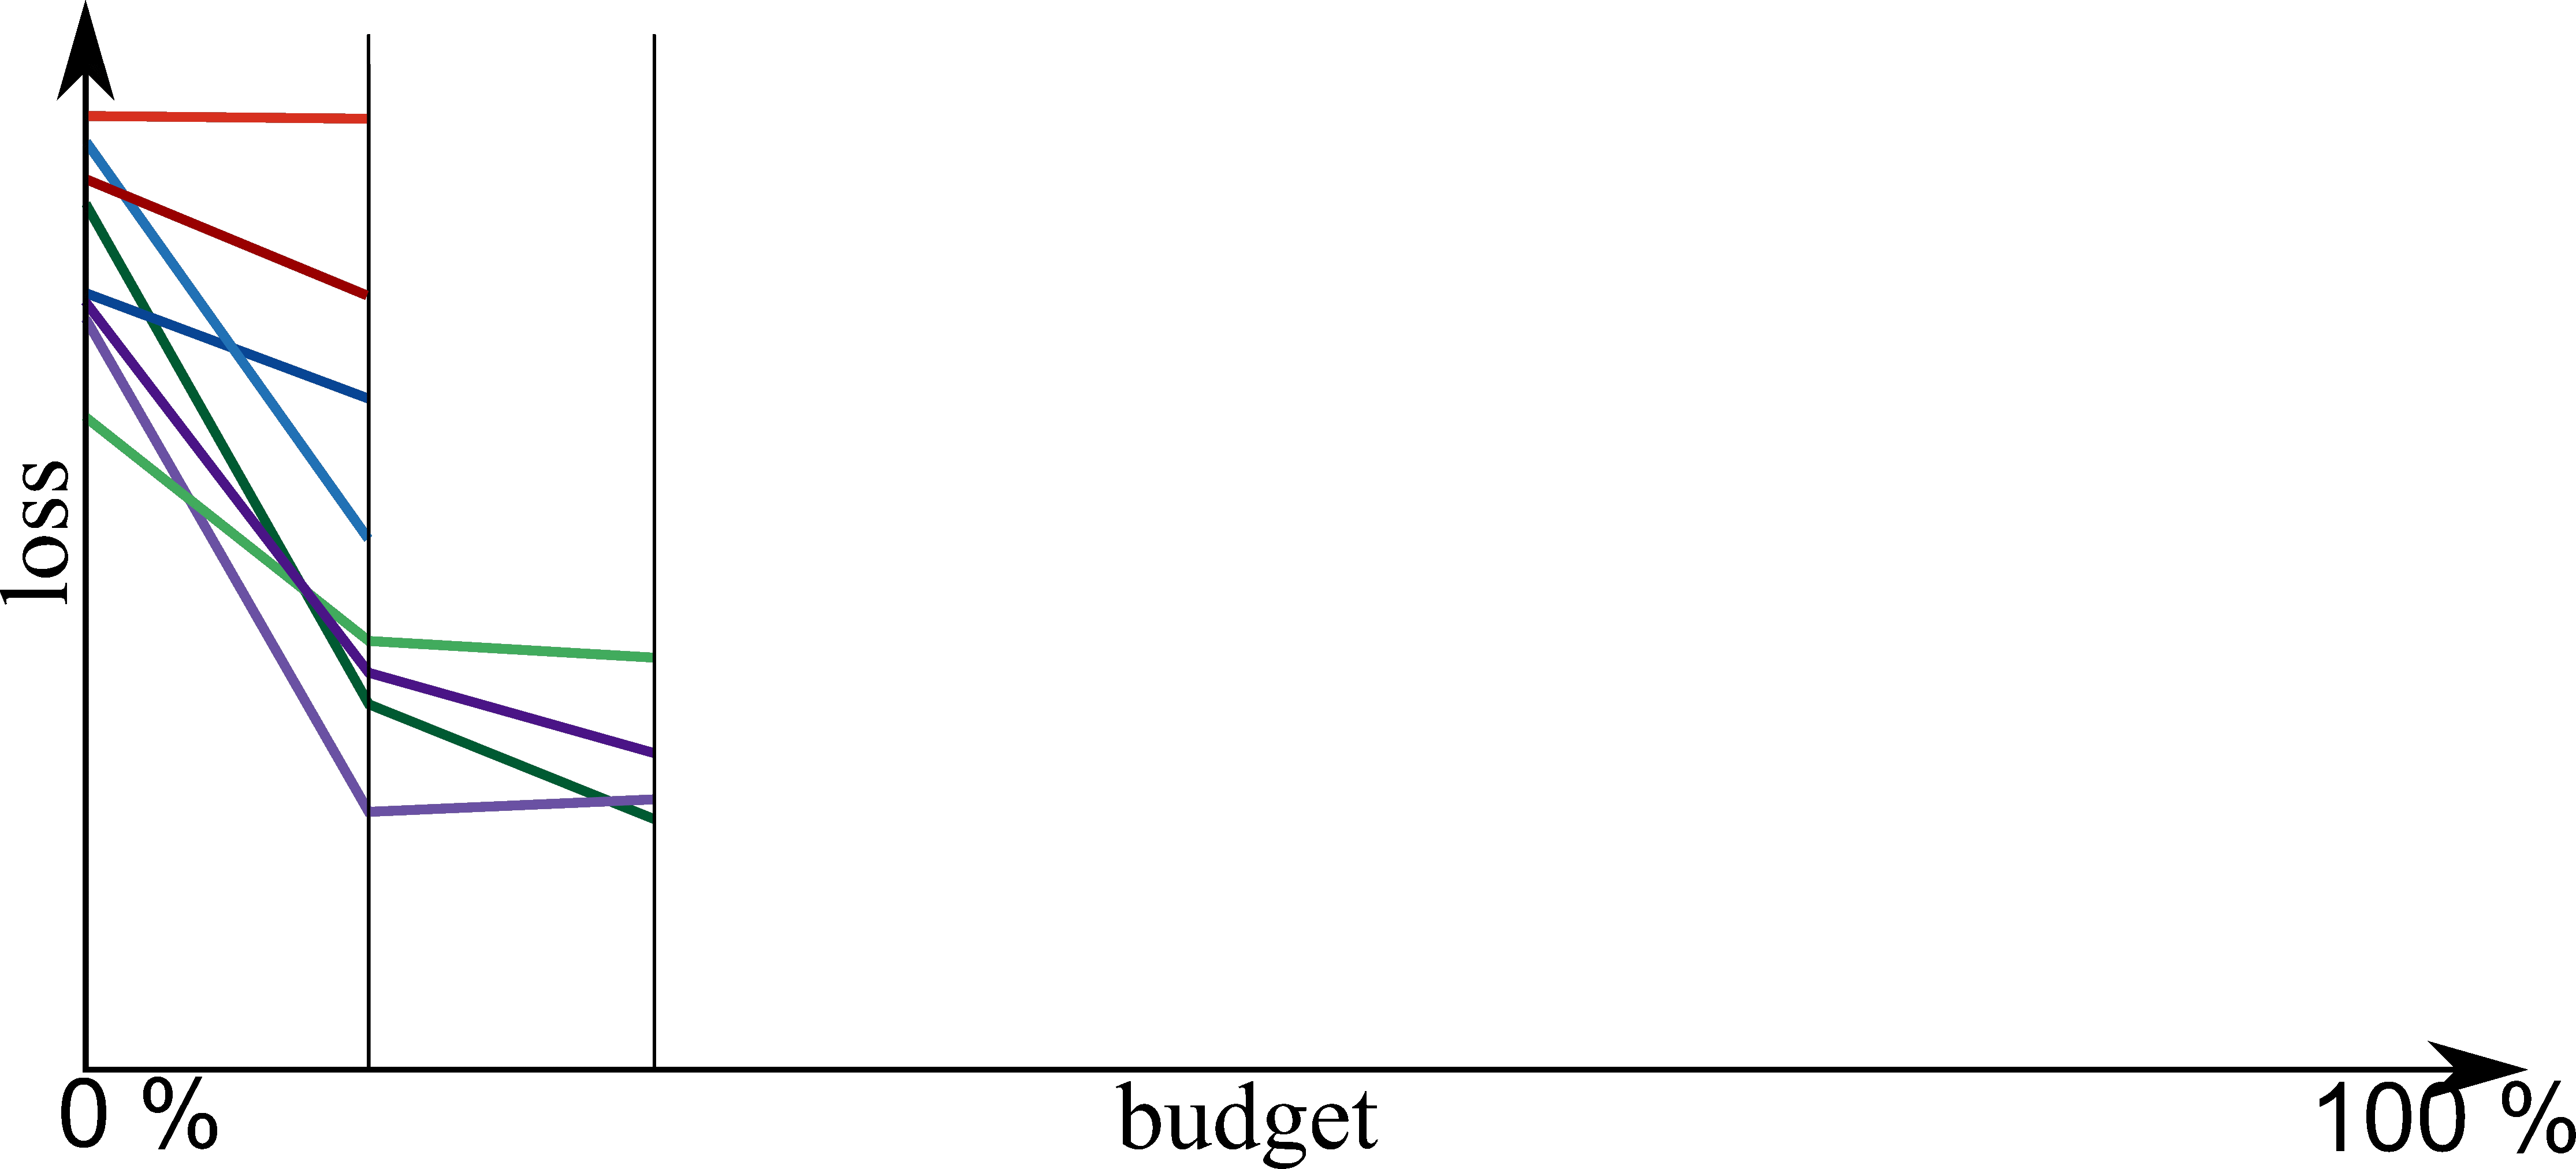
\includegraphics[width=\linewidth]{w07_hpo_grey_box/images/hyperband/SH-2.png}}
%     \only<5>{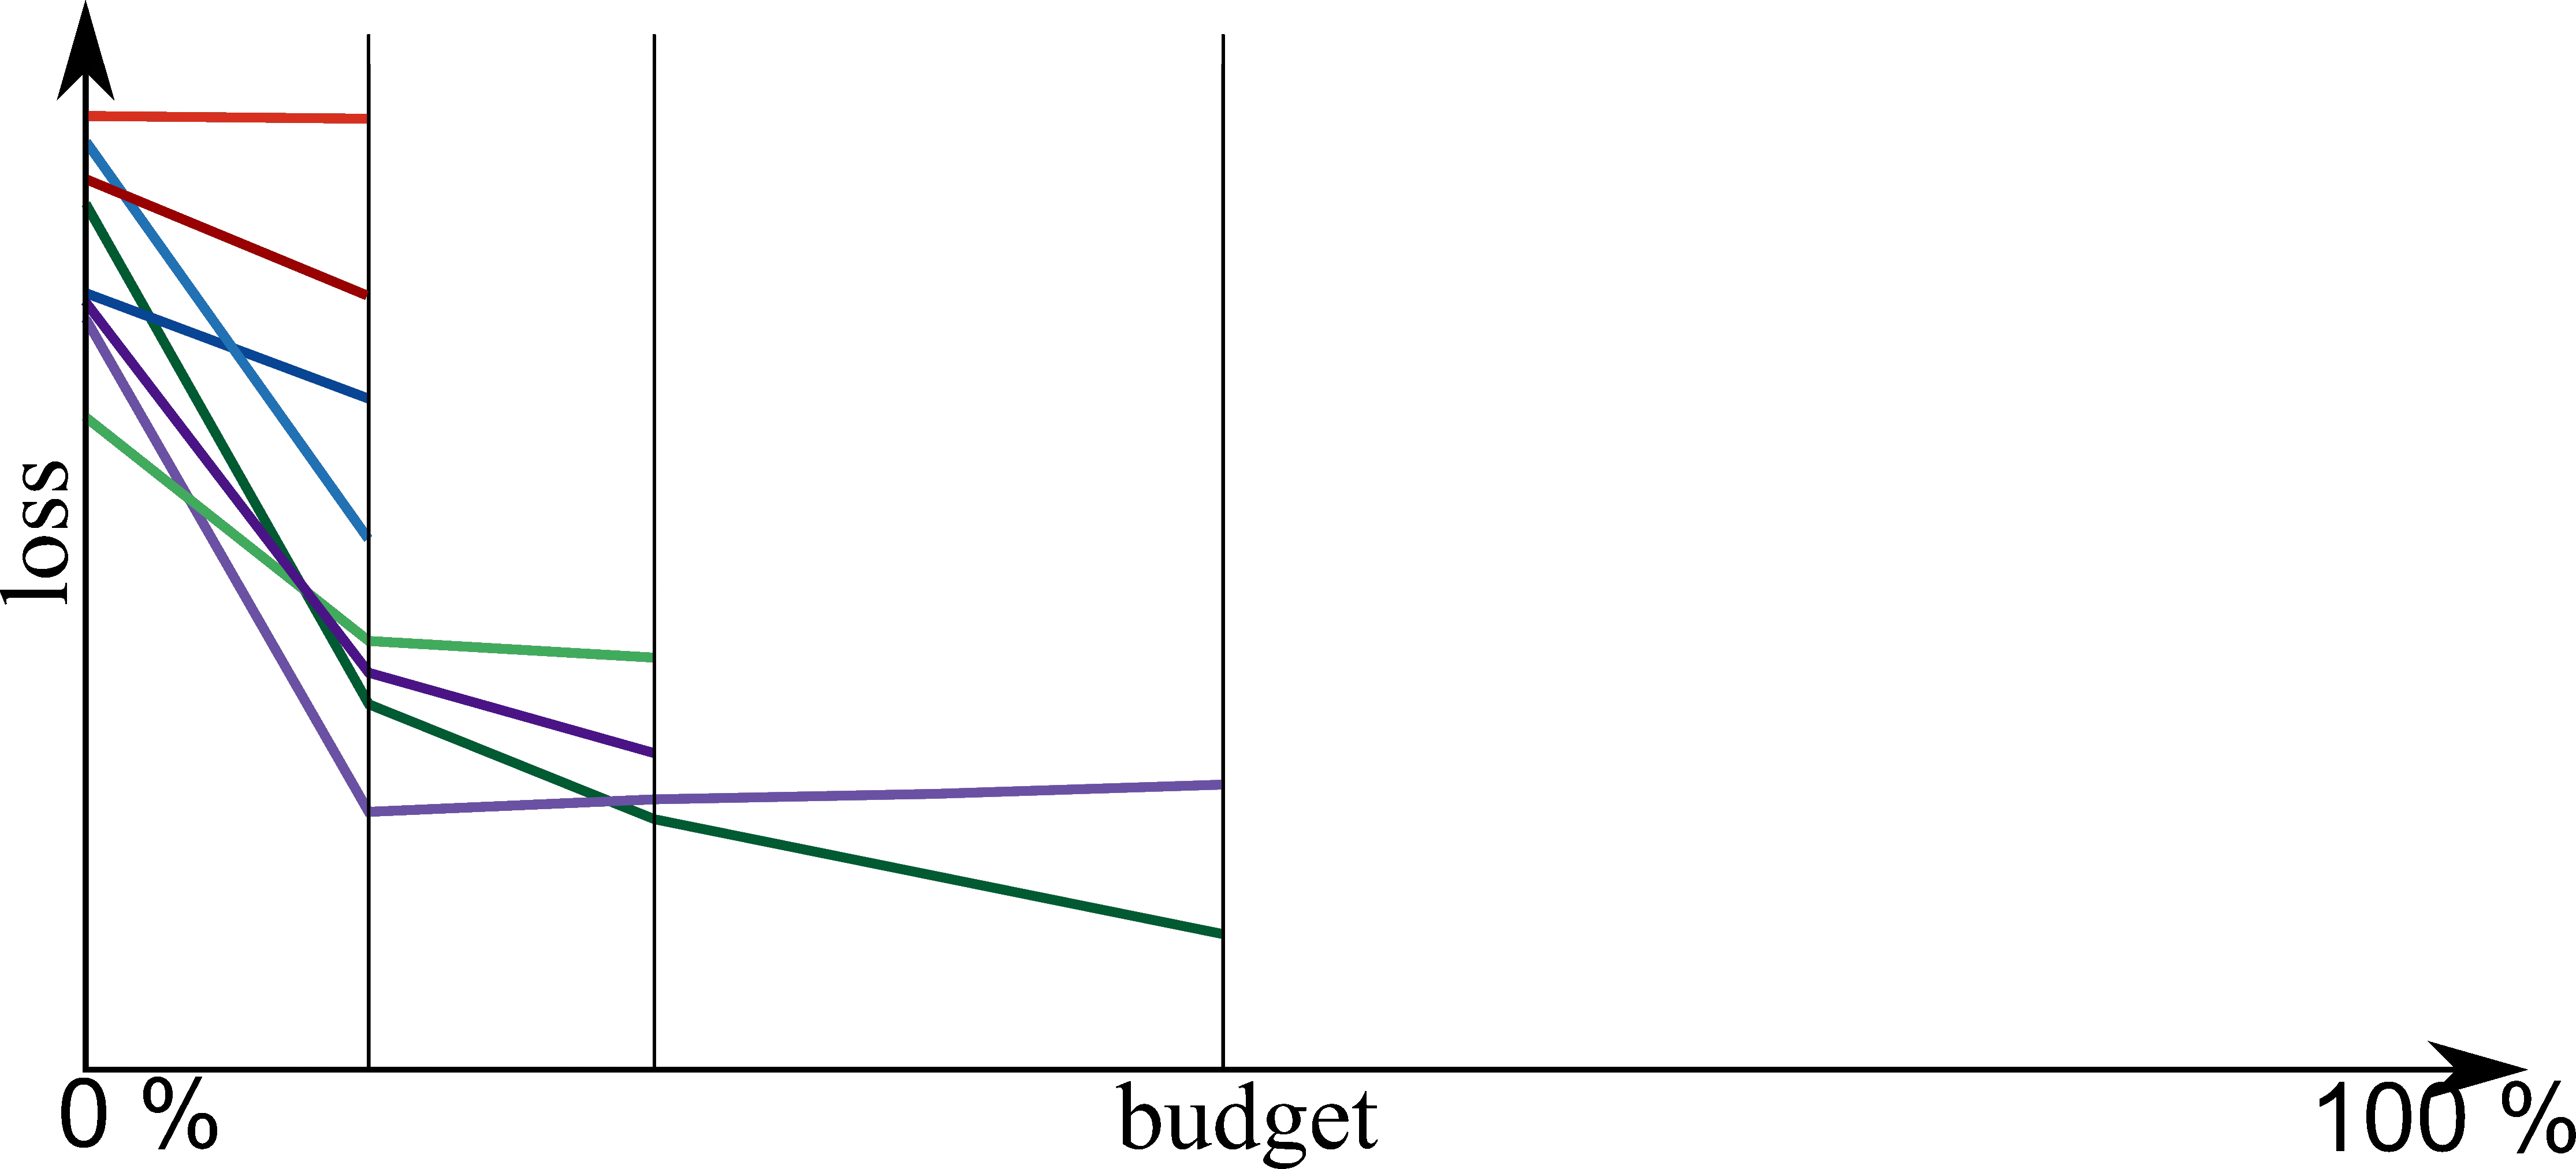
\includegraphics[width=\linewidth]{w07_hpo_grey_box/images/hyperband/SH-3.png}}
%     \only<6>{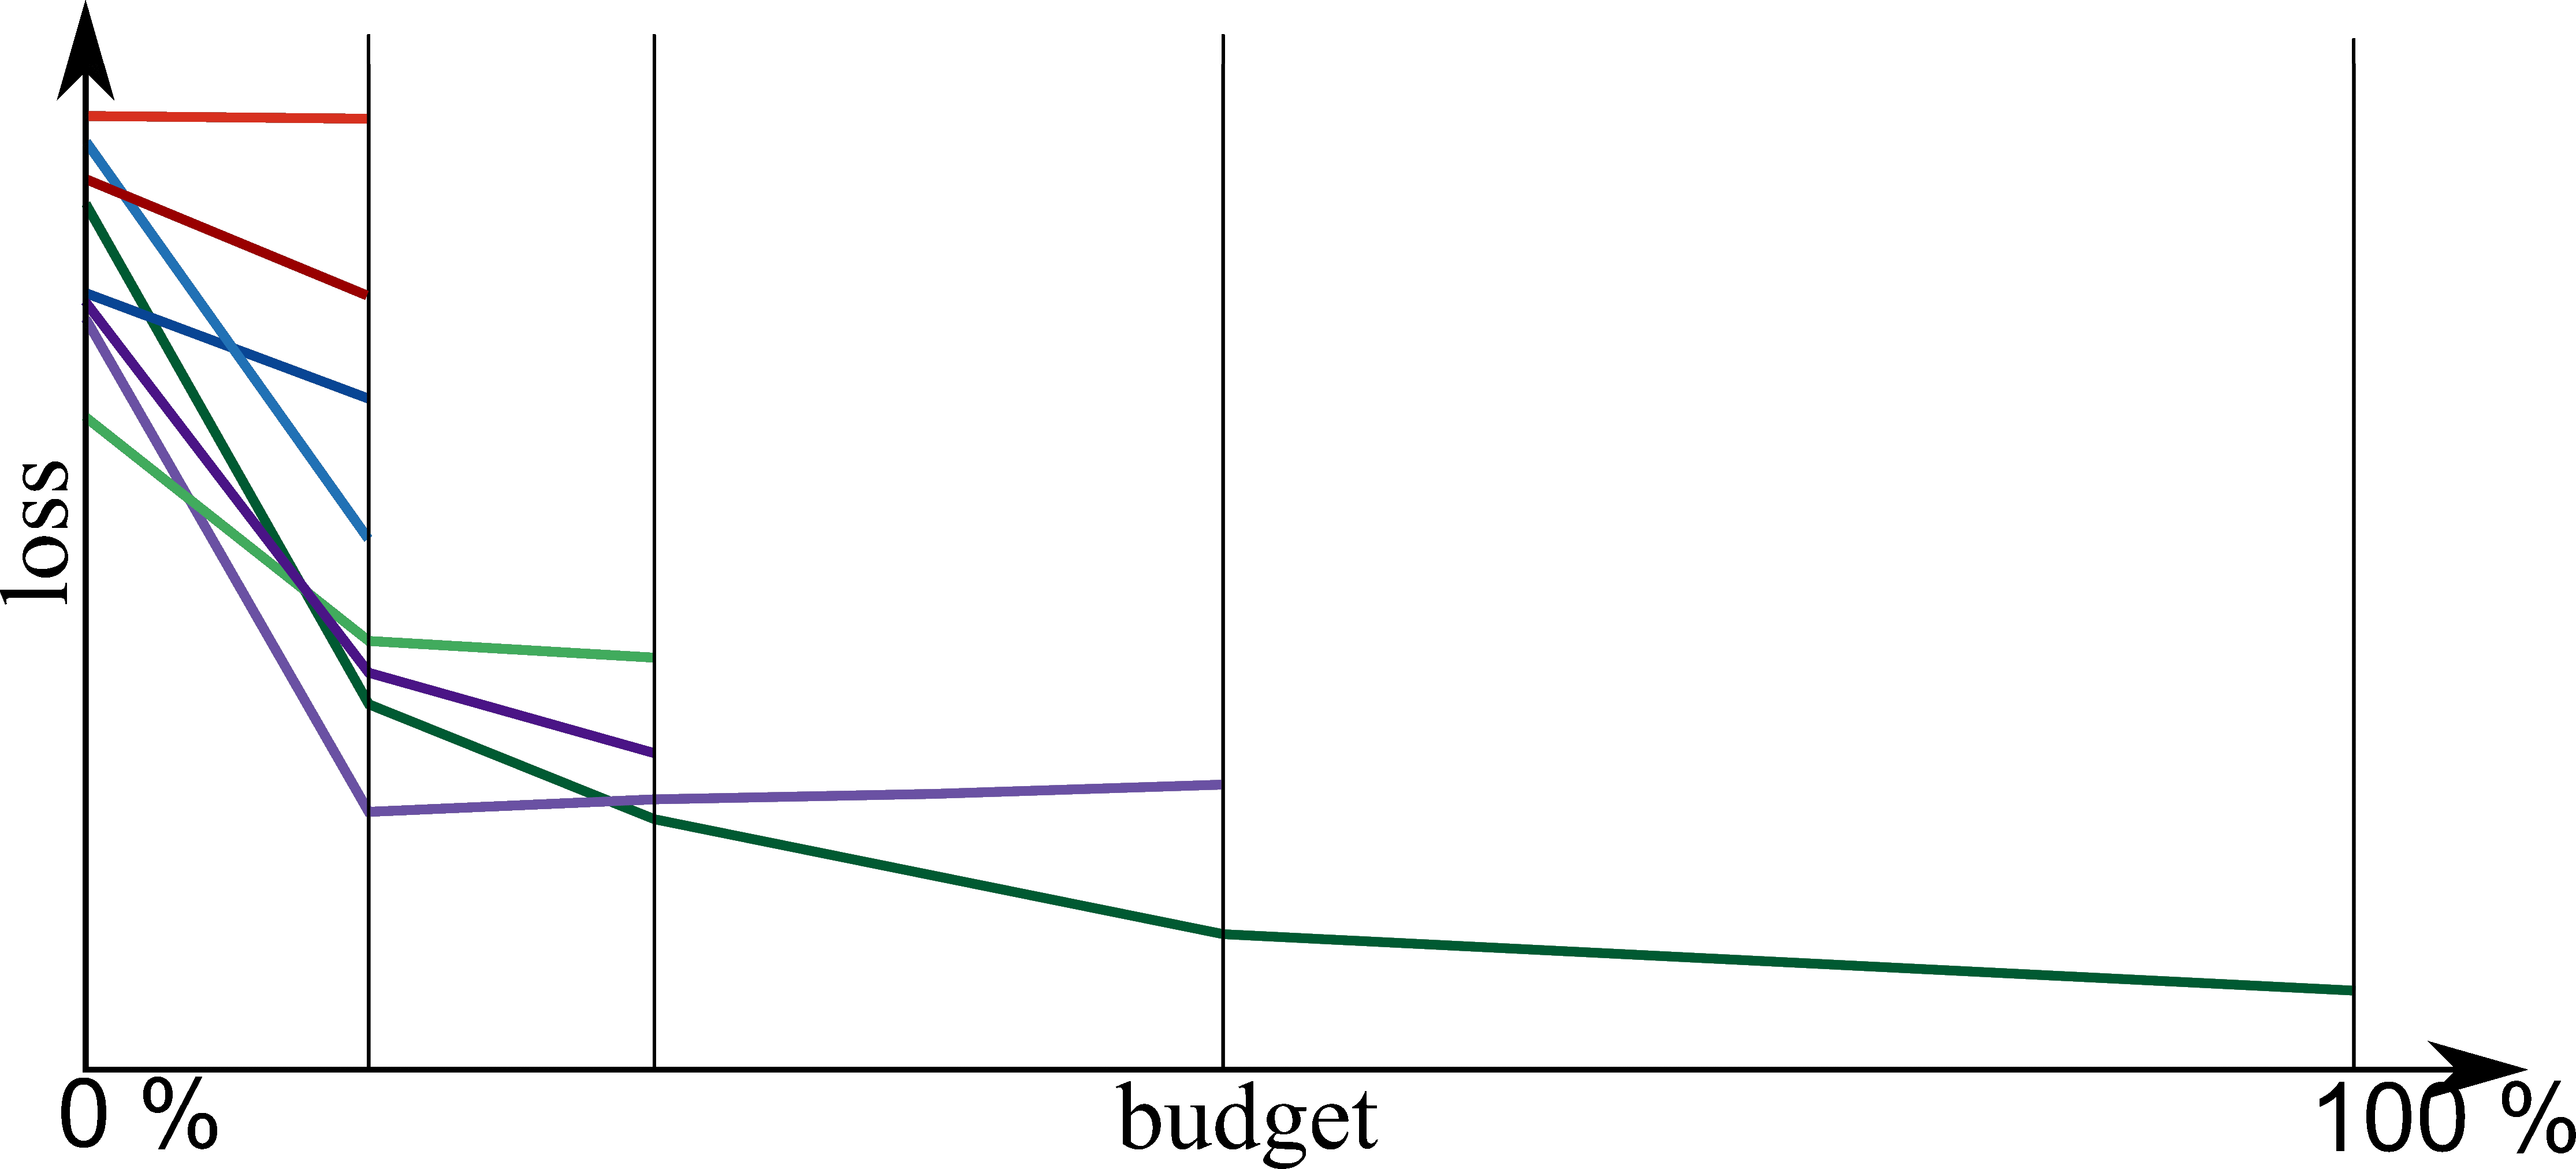
\includegraphics[width=\linewidth]{w07_hpo_grey_box/images/hyperband/SH-4.png}}

% \end{figure}
% \end{column}
% \end{columns}
% \vspace{-5em}
% \begin{columns}
% \begin{column}{.45\textwidth}
% Given a budget $B$ and the number of configurations $n$ as an input:
% \pause
% \begin{itemize}
%     \item Evaluate the performance of all configurations.
%     \pause
%     \item Drop the worst performing half.
%     \pause
%     \item Repeat until termination criterion is met e.g. maximum budget.

% \end{itemize}
% \end{column}

% \begin{column}{.45\textwidth}
% \end{column}

% \end{columns}

% \end{frame}

\begin{frame}{A Simple Multi-Fidelity Algorithms: Successive Halving (SH)}
\vskip -10pt
\hskip 270pt
\lit{\href{http://proceedings.mlr.press/v51/jamieson16.pdf}{Jamieson and Talwalkar, AISTATS 2016}}

\begin{columns}

    \column{0.8\textwidth}
    \begin{itemize}
        \item A very simple algorithm:
        \begin{itemize}
            \item Sample N configurations uniformly at random \& evaluate them on the cheapest fidelity
            \item Keep the best half (or third), move them to the next fidelity
            \item Iterate until the most expensive fidelity (= original expensive black box)
        \end{itemize}
    \end{itemize}
    
    \column{0.2\textwidth}
    \begin{figure}
        \centering
        \includegraphics[width=0.6\textwidth]{w07_hpo_grey_box/images/hyperband/black_blocks.png}
    \end{figure}

\end{columns}

\begin{figure}
    \centering
    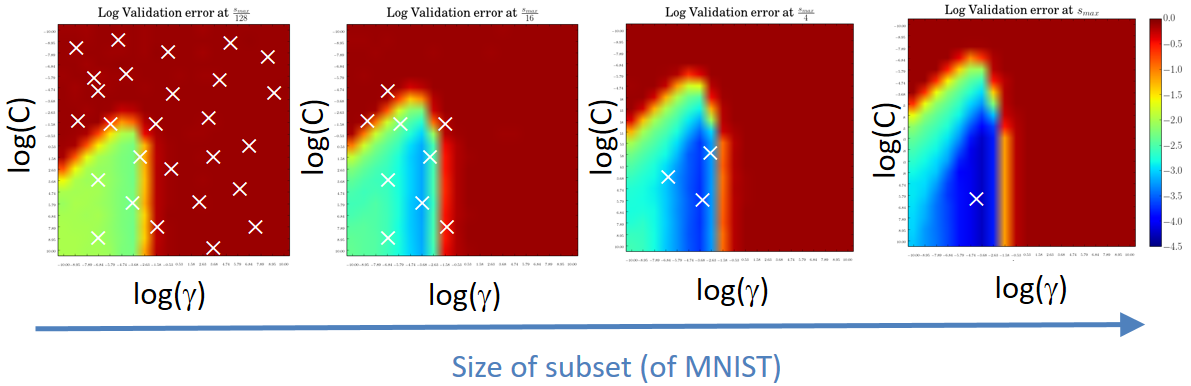
\includegraphics[width=0.8\textwidth]{w07_hpo_grey_box/images/hyperband/hyperband_fidelities.png}
\end{figure}
    
\end{frame}

%-----------------------------------------------------------------------
%-----------------------------------------------------------------------

\begin{frame}{The Same SH Algorithm When the Fidelity is Runtime}
\vskip -10pt
\hskip 270pt
\lit{\href{http://proceedings.mlr.press/v51/jamieson16.pdf}{Jamieson and Talwalkar, AISTATS 2016}}
    
\begin{figure}
    \centering
    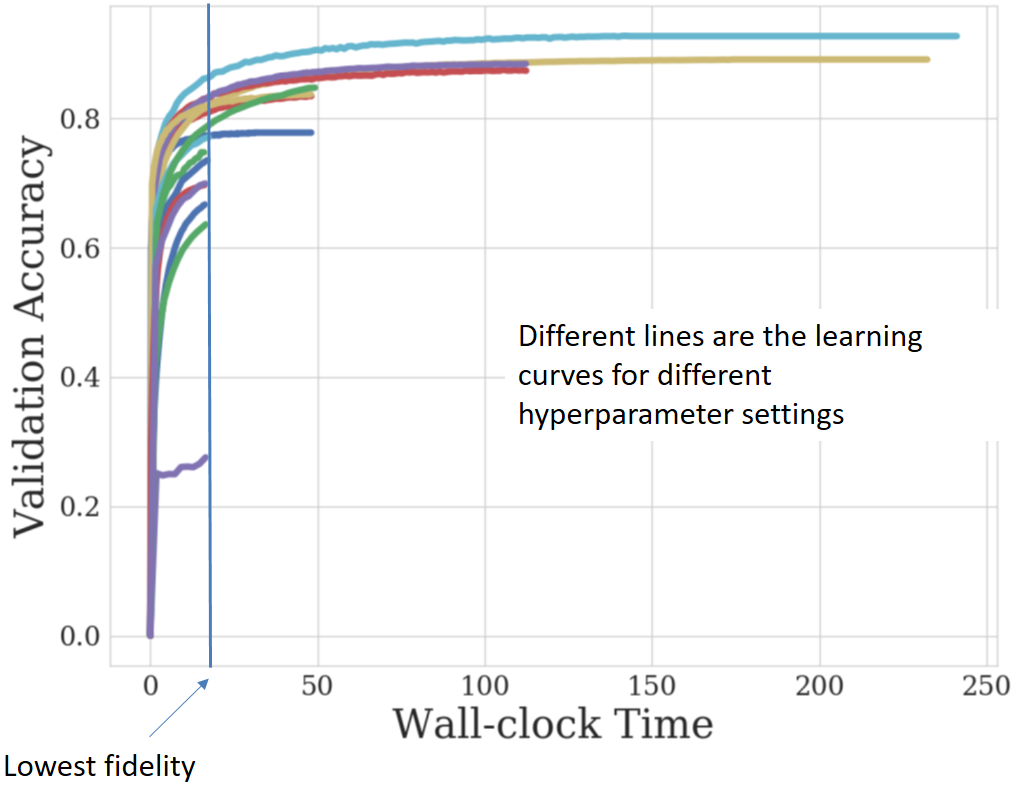
\includegraphics[width=0.6\textwidth]{w07_hpo_grey_box/images/hyperband/sh_accuracy_over_time.png}
\end{figure}
    
\end{frame}

%-----------------------------------------------------------------------
%-----------------------------------------------------------------------

\begin{frame}{Successive Halving(SH): Algorithm}
\begin{algorithm}[H]
    %\DontPrintSemicolon
    \LinesNumbered
    \SetAlgoLined
    \setcounter{AlgoLine}{0}
    \SetKwInOut{Input}{Input}
    \DeclarePairedDelimiter\ceil{\lceil}{\rceil}
    \DeclarePairedDelimiter\floor{\lfloor}{\rfloor}
    \DeclarePairedDelimiter\abs{\lvert}{\rvert}
    
    \Input{ initial budget $b_0,$ maximum budget $b_{max},$ set of $n$ configurations $C=\{\conf_1, \conf_2,\dots, \conf_{n}\}$}
    $b=b_0$\\
    \While{$b\leq b_{max}$}{
    $L=\{\Tilde{\cost}(\conf,b):\conf \in C\}$;\
    
    $C=top_{k}(C,L,\lfloor\lvert C \rvert\ / \eta \rfloor)$;\
    
    $b=\eta \cdot b$;\
    }
    
 
        
    
    \caption*{Pseudocode for SuccessiveHalving used by Hyperband as a subroutine}
\end{algorithm}

\end{frame}

%-----------------------------------------------------------------------

\begin{frame}{\emph{"n versus B/n" Problem}}
\begin{columns}

\begin{column}{.45\linewidth}
\begin{itemize}
    \item SH requires $B$ and $n$ as an input.
    \item Given finite $B$, $B/n$ resources are allocated across the configurations.
    \item Configurations need enough minimal resources to differentiate between them in terms of quality.
\end{itemize}
\end{column}

\begin{column}{.45\linewidth}

\begin{figure}
    \centering
    \vspace{2em}
    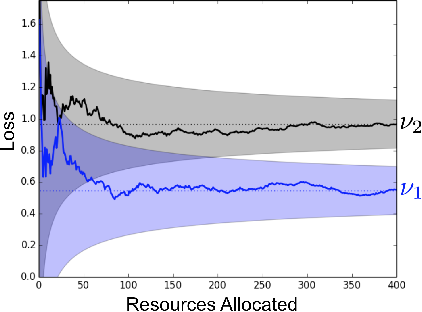
\includegraphics[width=0.9\linewidth]{w07_hpo_grey_box/images/intro/differetiatingConfigurations.png}
\end{figure}
\end{column}
\end{columns}

\vspace{-6.5em}
\begin{columns}

\begin{column}{.45\linewidth}
\begin{itemize}

    \item Issue: Optimal allocation strategy is unknown in practice.
    \item Idea: Perform grid search over a feasible set of tuples of $n$ and minimal resource $r$. (Hyperband) 
\end{itemize}
\end{column}

\begin{column}{.45\linewidth}

\end{column}
    
\end{columns}
    
\end{frame}

% %-----------------------------------------------------------------------
% \begin{frame}{Hyperband}
% \begin{itemize}
%     \item Issue of successive halving (for a fixed B):
%     \begin{itemize}
%         \item Do you want to run many configurations with aggressive rejection?
%         \item Or: Do you want to run few configurations with non-aggressive rejection?
%     \end{itemize}
%     \item Ideas:
%     \begin{itemize}
%         \item Add an outer loop to try different trade-offs between $\#$configurations and budget.
%         \item Add further parameter: proportion of configurations discarded in each round of successive halving
%     \end{itemize}
%     \item Starts with many configurations that gets aggressively rejected.
%     \item In later iterations, fewer configurations with more budget each.
%     \item Returns: configuration with the smallest intermediate loss seen so far.
% \end{itemize}
% \end{frame}

%-----------------------------------------------------------------------

\begin{frame}{An Extension of SH with Theoretical Guarantees: Hyperband}
    
\vskip -10pt
\hskip 330pt
\lit{\href{http://jmlr.org/papers/v18/16-558.html}{Li et al., JMLR 2018}}
    
\begin{columns}

    \column{0.25\textwidth}
    \begin{itemize}
        \item Main Idea: \\ hedge against errors in cheap approximations
        \item Algorithm: \\ run multiple copies of SH in parallel, starting at different cheapest fidelities
    \end{itemize}
    
    \column{0.75\textwidth}
    \vskip -20pt
    \begin{figure}
        \centering
        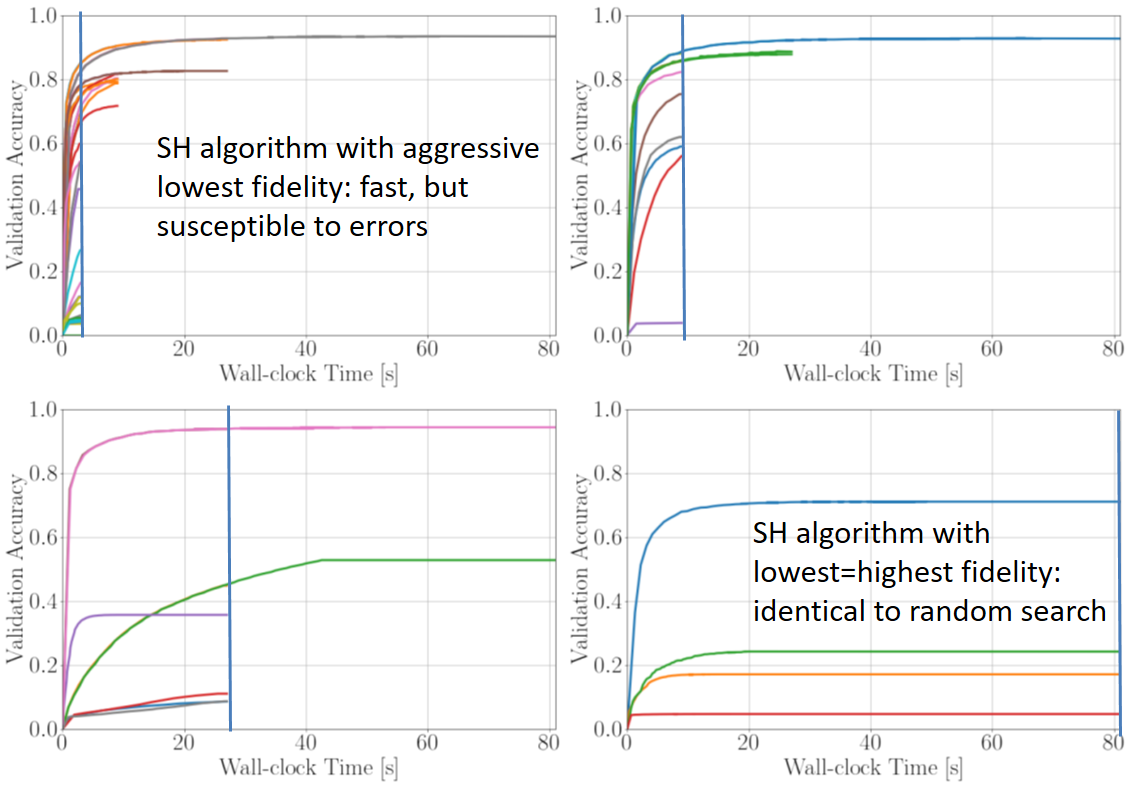
\includegraphics[width=0.9\textwidth]{w07_hpo_grey_box/images/hyperband/hyperband_illustration.png}
    \end{figure}

\end{columns}
    
\end{frame}

%-----------------------------------------------------------------------

\begin{frame}{Hyperband: Algorithm}
\begin{minipage}{0.75\textwidth}
\begin{algorithm}[H]
    %\DontPrintSemicolon
    \LinesNumbered
    \SetAlgoLined
    \setcounter{AlgoLine}{0}
    \DeclarePairedDelimiter\ceil{\lceil}{\rceil}
    \DeclarePairedDelimiter\floor{\lfloor}{\rfloor}
    
    \Input{budgets $b_{min}$ and $b_{max}, \eta$}
    
    $s_{max}=\floor*{\log_{\eta}\frac{b_{max}}{b_{min}}}$;\
    
    \For{$s\in \{s_{max}, s_{max}-1, \dots, 0\}$}
    {
        sample $\eta=\lceil\frac{s_{max}+1}{s+1} \cdot\eta^{s}\rceil$;\
        
        run SH on them with $\eta^{s}\cdot b_{max}$;\
    }
 
        
    
    \caption*{Pseudocode for Hyperband using SuccessiveHalving (SH) as a subroutine}
\end{algorithm}
\end{minipage}
\end{frame}
% %-----------------------------------------------------------------------
% %-----------------------------------------------------------------------
% \begin{frame}{Tradeoffs between n and B/n}
% \vspace{2em}
% \begin{figure}
%     \centering
%     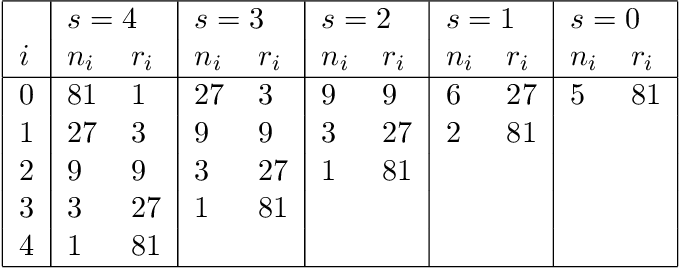
\includegraphics[width=0.7\textwidth]{w07_hpo_grey_box/images/hyperband/Hyperband_Table1-1.png}
%     \caption{The values of $n_i$ and $r_i$ for the brackets of Hyperband corresponding to various values of $s$, when $R = 81$ and $\eta = 3$.}
% \end{figure}

    
% \end{frame}

% %-----------------------------------------------------------------------
% %-----------------------------------------------------------------------
% \begin{frame}{Empirical comparison between individual brackets}
% \begin{figure}
%     \centering
%     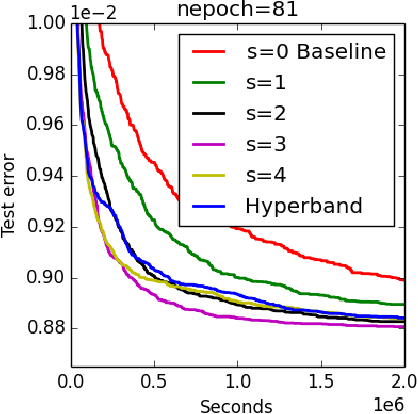
\includegraphics[width=0.4\textwidth]{w07_hpo_grey_box/images/hyperband/Hyperband_figure_3.png}
%     \caption{Performance of individual brackets $s$ and Hyperband.}
% \end{figure}
% \begin{itemize}
%     \item Hyperband is slower than SuccessiveHalving by a small factor if aggressive early-stopping is not suitable for the task.
% \end{itemize}

    
% \end{frame}

% %-----------------------------------------------------------------------
% \begin{frame}{Hyperband: Comparison}
% \begin{figure}
%     \centering
%     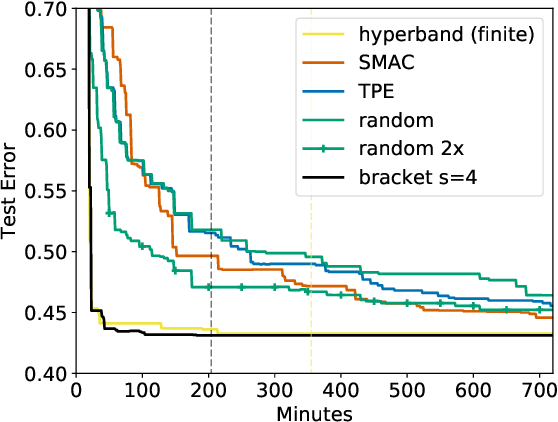
\includegraphics[width=0.55\textwidth]{w07_hpo_grey_box/images/hyperband/Figure_experiments.png}
%     \caption{Average test error of the best kernel regularized least square classification model found by each searcher on CIFAR-10.}
% \end{figure}

    
% \end{frame}

%-----------------------------------------------------------------------

%-----------------------------------------------------------------------
\begin{frame}{Empirical Evaluation: Hyperband vs. Random Search}

\vskip -10pt
\hskip 270pt
\lit{\href{http://proceedings.mlr.press/v80/falkner18a/falkner18a.pdf}{Falkner, Klein \& Hutter, ICML 2018}}

\begin{figure}
    \centering
    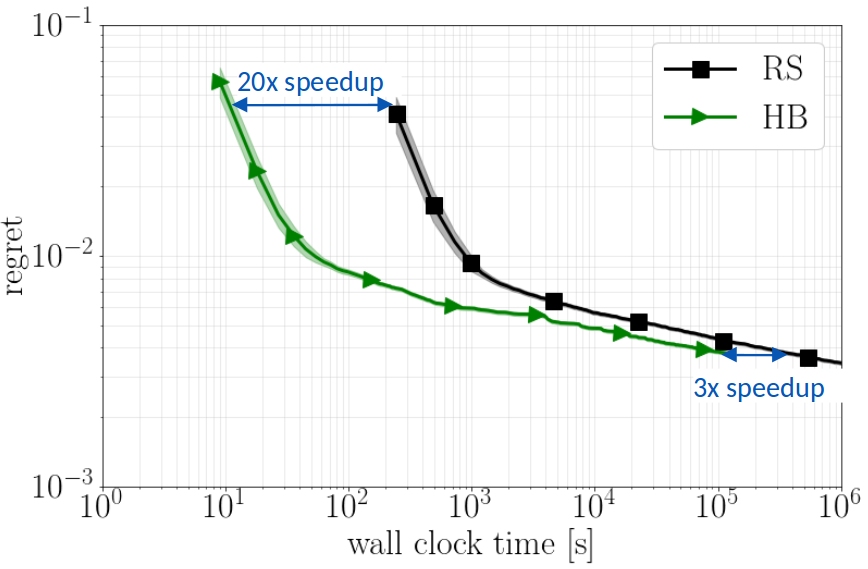
\includegraphics[width=0.7\textwidth]{w07_hpo_grey_box/images/hyperband/bohb_2.png}
\end{figure}

\begin{center}
    Biggest advantage: much improved \emph{anytime performance}
    
    \tiny{Auto-Net on dataset adult}
\end{center}

\end{frame}

%-----------------------------------------------------------------------
\begin{frame}{Random Search vs. Hyperband}

\begin{itemize}
    \item In practice HB performs very well for small to medium budgets
    \item Outperforms random search and vanilla BO
    \item However, its convergence is limited by its reliance on randomly-drawn configurations
    \item With larger budgets its advantage over random search diminishes
\end{itemize}
\begin{figure}
    \centering
    \includegraphics[width=0.6\textwidth]{w07_hpo_grey_box/images/hyperband/comparison_rs_hb.png}
\end{figure}


\end{frame}

%-----------------------------------------------------------------------

%-----------------------------------------------------------------------
\begin{frame}{Questions to Answer for Yourself / Discuss with Friends}

\bigskip

\begin{itemize}
    \item \alert{Repetition.} Why can't one simply use both a large $B$ and $n$ for doing hyperparameter optimization?

\medskip
    \item \alert{Discussion.} 
    Can you think of settings where the stopping heuristic is futile?

\end{itemize}

\end{frame}
%----------------------------------------------------------------------
%----------------------------------------------------------------------	
%\videotitle{BOHB}
%----------------------------------------------------------------------

\begin{frame}[c]{Robust and Efficient Hyperparameter Optimization at Scale}
Desiderata for a practical solution to the hyperparamenter optimization problem:
\begin{itemize}
    \item Strong Anytime Performance
    \item Strong Final Performance
    \pause
    \item Scalability
    \item Robustness $\&$ Flexibility
    \pause
    \item Computational Efficiency
    \item Effective Use of Parallel Resources
    \pause
    \item Conceptual / Algorithmic Simplicity
    \pause
\end{itemize}
\bigskip
To fulfill all of these desiderata, BOHB \lit{\href{http://proceedings.mlr.press/v80/falkner18a.html}{Falkner, Klein and Hutter, ICML 2018}} combines Bayesian Optimization with Hyperband 

\end{frame}
%-----------------------------------------------------------------------
%----------------------------------------------------------------------
\begin{frame}[c]{BOHB}
\begin{itemize}
    \item BOHB combines the advantages of Bayesian Optimization and Hyperband
    \myit{
        \item Bayesian Optimization for choosing configurations to achieve strong final performance
        \item Hyperband to choose the budgets for good anytime performance    
    }
\pause
\bigskip
    \item BOHB replaces the random selection of configurations at the beginning of each HB iteration by a model-based search
\pause
\bigskip
    \item Details of the model
    \myit{
        \item Variant of the Tree Parzen Estimator, with a product kernel
        \item Models are fitted independently to the data for one budget at a time
        \myit{
            \item Specifically, always the highest budget that has enough data points
        }
    }
\end{itemize}

\end{frame}
%-----------------------------------------------------------------------
%----------------------------------------------------------------------
%\begin{frame}[c]{BOHB}
%\begin{itemize}
%    \item Strong anytime performance of BOHB(desideratum 1) stems from its use of Hyperband.
%    \begin{itemize}
%        \item Quickly evaluating lots of configurations on small budgets allows BOHB to quickly identify promising configurations.
%        \pause
%    \end{itemize}
%    \item The strong final performance (desideratum 2) stems from BOHB's BO part as the guided search is able to refine the selected configurations.
%    \pause
%    \item BOHB also efficiently takes advantage of parallel resources (desideratum 3).
%    \begin{itemize}
%        \item In each iteration BOHB is evaluations multiple configurations, which can be independently run on multiple workers.
%        \item The parallelism in TPE is achieved by limiting the number of samples to optimize EI.
%        \item Single pool of workers, and whenever a worker becomes available preferentially execute waiting runs with smaller budgets.
%    \end{itemize}
%\end{itemize}
%
%\end{frame}
%-----------------------------------------------------------------------
%----------------------------------------------------------------------
\begin{frame}{BOHB: Algorithm}

\begin{centering}
\begin{minipage}{0.75\textwidth}
\begin{algorithm}[H]
    %\DontPrintSemicolon
    \LinesNumbered
    \SetAlgoLined
    \setcounter{AlgoLine}{0}
    \DeclarePairedDelimiter\ceil{\lceil}{\rceil}
    \DeclarePairedDelimiter\floor{\lfloor}{\rfloor}
    \DeclarePairedDelimiter\abs{\lvert}{\rvert}
    
    \Input{observations D, fraction of random runs $\rho$, percentile $q$, number of samples $N_s$,
     minimum number of points $N_{min}$ to build a model, and bandwidth factor $b_w$}
    \Output{next configuration to evaluate}
    \lIf{$rand()<\rho$}{\Return{random configuration}}
    $b=\argmax \{D_b:\lvert D_b \rvert \geq N_{min}+2\}$
    
    \lIf{$b=\varnothing$}{\Return{random configuration}}
    
    Fit KDEs according to Equation~\ref{eq:TPE_Densities}
    
    Draw $N_s$ samples acoording to $l'(\conf)$
    
    \Return{sample with highest ratio $l(\conf)/g(\conf)$}
       
    
    \caption*{Pseudocode for sampling in BOHB}
\end{algorithm}
\end{minipage}
\end{centering}

%\vspace{-2em}
\begin{equation}
    l(\conf)=p(\obs<\alpha| D_b)\quad\quad\quad\quad
    g(\conf)=p(\obs>\alpha| D_b)
    \label{eq:TPE_Densities}
\end{equation}

\begin{itemize}
    \item To optimize EI, we sample $N_s$ points from $l^{'}(\conf)$ which is $l(\conf)$ but with all bandwidths multiplied by a factor $b_w$ to encourage more exploration around the promising configurations.
\end{itemize}

\end{frame}
%-----------------------------------------------------------------------
%----------------------------------------------------------------------
\begin{frame}{BOHB: Comparison}
\begin{figure}
    \centering
    \includegraphics[width=0.68\textwidth]{../w07_hpo_speedup/images/bohb/BOHB_1.pdf}
    \caption{Performance of RS and BOHB on Auto-Net on datasted Adult}
\end{figure}

\end{frame}
%-----------------------------------------------------------------------
%----------------------------------------------------------------------
\begin{frame}{BOHB: Comparison}
\begin{figure}
    \centering
    \includegraphics[width=0.68\textwidth]{../w07_hpo_speedup/images/bohb/BOHB_2.pdf}
    \caption{Performance of RS and BOHB on Auto-Net on datasted Adult}
\end{figure}

\end{frame}
%-----------------------------------------------------------------------
%----------------------------------------------------------------------
\begin{frame}{BOHB: Comparison}
\begin{figure}
    \centering
    \includegraphics[width=0.68\textwidth]{../w07_hpo_speedup/images/bohb/BOHB_3.pdf}
    \caption{Performance of RS and BOHB on Auto-Net on datasted Adult}
\end{figure}

\end{frame}
%-----------------------------------------------------------------------
%----------------------------------------------------------------------
\begin{frame}{BOHB: Comparison}
\begin{figure}
    \centering
    \includegraphics[width=0.68\textwidth]{../w07_hpo_speedup/images/bohb/BOHB_4.pdf}
    \caption{Performance of RS, TPE, HB and BOHB on Auto-Net on datasted Adult}
\end{figure}

\end{frame}
%-----------------------------------------------------------------------
%----------------------------------------------------------------------
\begin{frame}{BOHB: Different number of parallel workers}
\begin{figure}
    \centering
    \includegraphics[width=0.70\textwidth]{../w07_hpo_speedup/images/bohb/parallelization_letter.png}
    \caption{Performance of BOHB with different number of parallel workers on the letter surrogate benchmark for 128 iterations}
\end{figure}

\end{frame}
%-----------------------------------------------------------------------
%----------------------------------------------------------------------
\begin{frame}{BOHB: Optimization of a Bayesian neural network}
\begin{figure}
    \centering
    \includegraphics[width=0.70\textwidth]{../w07_hpo_speedup/images/bohb/bnn_boston-1.png}
    \caption{Optimization of 5 hyperparameters of a Bayesian neural network trained with SGHMC.}
\end{figure}

\end{frame}
%-----------------------------------------------------------------------
%----------------------------------------------------------------------
\begin{frame}{BOHB: Optimization of a reinforcement learning agent}
\begin{figure}
    \centering
    \includegraphics[width=0.70\textwidth]{../w07_hpo_speedup/images/bohb/cartpole-1.png}
    \caption{Hyperparameter optimization of 8 hyperparameters of PPO on the cartpole task.}
\end{figure}

\end{frame}
%-----------------------------------------------------------------------
%----------------------------------------------------------------------
\begin{frame}{BOHB: Optimization of an SVM}
\begin{figure}
    \centering
    \includegraphics[width=0.70\textwidth]{../w07_hpo_speedup/images/bohb/svm_surrogate_test_pdf-1.png}
    \caption{Comparison on the SVM on MNIST surrogates}
\end{figure}

\end{frame}
%-----------------------------------------------------------------------
%----------------------------------------------------------------------
\begin{frame}{BOHB: Counting Ones }
\begin{figure}
    \centering
    \includegraphics[width=0.70\textwidth]{../w07_hpo_speedup/images/bohb/countingones_bohb.png}
    \caption{Results for the counting ones problem in 16 dimensional
space with 8 categorical and 8 continuous hyperparameters.}
\end{figure}

\end{frame}
%-----------------------------------------------------------------------
%----------------------------------------------------------------------
\begin{frame}{BOHB: Surrogate on poker }
\begin{figure}
    \centering
    \includegraphics[width=0.70\textwidth]{../w07_hpo_speedup/images/bohb/surrogate_on_poker.png}
    \caption{Optimizing six hyperparameter of a feed-forward neural
network on featurized datasets; results are based on surrogate
benchmarks. }
\end{figure}

\end{frame}
%-----------------------------------------------------------------------

%-----------------------------------------------------------------------
\begin{frame}{Questions to Answer for Yourself / Discuss with Friends}

\bigskip

\begin{itemize}
    \item \alert{Repetition.} Why does BOHB interleave randomly sampled configurations in the optimization process?

\medskip
    \item \alert{Discussion.} 
    What are the advantages of the Parzen estimator model over more advanced models such as random forests or Gaussian processes?

\end{itemize}

\end{frame}
%----------------------------------------------------------------------
%----------------------------------------------------------------------
%\videotitle{Success Stories}

%----------------------------------------------------------------------
\begin{frame}[c]{Spearmint \litw{\href{https://papers.nips.cc/paper/4522-practical-bayesian-optimization-of-machine-learning-algorithms.pdf}{Snoek et al. 2012}}}

\small
\begin{itemize}
    \item First successful open source Bayesian optimization implementation     
%    \item Was used to tune a neural network to state-of-the-art performance on CIFAR-10 in 2012
    \item Implements standard Bayesian optimization with MCMC integration of the acquisition function, asynchronous parallelism, 
    input warping 
    and constraints
    \item \alert{Startup based on Spearmint got acquired by Twitter in 2015}
    \item Still heavily used and cited and available at \url{https://github.com/HIPS/spearmint}:
    \begin{center}
        \only{\includegraphics[width=0.7\linewidth, keepaspectratio=true]{images/success_stories/jsnoek_spearmint_git_stats.png}}
        
        \only{\includegraphics[width=0.7\linewidth, keepaspectratio=true]{images/success_stories/hips_spearmint_git_stats.png}}
        
        \only{\includegraphics[width=.5\linewidth, keepaspectratio=true]{images/success_stories/spearmint_alt_stats.png}}
%        \newline Google Scholar screenshot from 3rd March, 2020
    \end{center}
\end{itemize}
\end{frame}

%-----------------------------------------------------------------------
\begin{frame}[c]{Hyperopt \litw{\href{https://papers.nips.cc/paper/4443-algorithms-for-hyper-parameter-optimization.pdf}{Bergstra et al. 2011}; \href{http://proceedings.mlr.press/v28/bergstra13.pdf}{Bergstra et al. 2013}; \href{http://citeseerx.ist.psu.edu/viewdoc/download?doi=10.1.1.704.3494&rep=rep1&type=pdf}{Bergstra et al. 2013}; \href{https://iopscience.iop.org/article/10.1088/1749-4699/8/1/014008/ampdf}{Bergstra et al. 2015}}}
\begin{itemize}
    \item Hyperopt is another successful open source Bayesian optimization package
    \item Implements the TPE algorithm and supports asynchronous parallel evaluations
    \item Maintained since 2013
    \item Available at \url{https://github.com/hyperopt/hyperopt}
\end{itemize}
\vspace{1cm}
\includegraphics[width=\linewidth, height=\textheight, keepaspectratio=true]{images/success_stories/hyperopt_git_stats.png}

\vspace{1cm}
\hspace{2cm}


\end{frame}

%---------------------------------------------------------------------
\begin{frame}[c]{SMAC  \litw{\href{https://ml.informatik.uni-freiburg.de/papers/11-LION5-SMAC.pdf}{Hutter et al. 2011}}}

\begin{itemize}
    \item Standard BO tool based on random forests (RFs), reflecting the strengths of RFs in terms of \alert{scalability \& flexibility}:
    \begin{itemize}
        \item High dimensionality (low effective dimensionality)
        \item Computational efficiency ($\rightarrow$ low overhead)
        \item Supports continuous/categorical/conditional parameters
        \item Supports non-standard noise (non-Gaussian, heteroscedastic)
        \item Usability off the shelf (robustness towards model's own hyperparameters)
    \end{itemize}

\fhpause
\smallskip
    \item SMAC also handles a more general problem:
    $\argmin_{\conf\in\confs} \sum_{i=1}^N \cost(\conf,i)$
\fhpause
\smallskip
    \item Maintained since 2011, now available in version 3: \url{https://github.com/automl/SMAC3}

\begin{columns}
\column{0.05\textwidth}
\column{0.45\textwidth}
~\\
%\vspace*{0.1cm}
\includegraphics[width=1\linewidth, keepaspectratio=true]{images/success_stories/SMAC_citations.png}
\column{0.45\textwidth}
~\\
~\\
~\\
\includegraphics[width=1\linewidth, keepaspectratio=true]{images/success_stories/SMAC_paper.png}
~\\
\column{0.05\textwidth}
\end{columns}    
\end{itemize}
\end{frame}
%----------------------------------------------------------------------

%-----------------------------------------------------------------------
\begin{frame}[c]{Tuning AlphaGo \litw{\href{https://arxiv.org/pdf/1812.06855.pdf}{Chen et al. 2018}}}
\begin{itemize}
    \item ``During the development of AlphaGo, \alert{its many hyperparameters were tuned with Bayesian optimization multiple times.}''
\medskip
    \item ``This automatic tuning process resulted in \alert{substantial improvements in playing strength}. For example, prior to the match with Lee Sedol, we tuned the latest AlphaGo agent and this \alert{improved its win-rate from 50\% to 66.5\%} in self-play games. \alert{This tuned version was deployed in the final match.}
\medskip
    \item Of course, since we tuned AlphaGo many times during its development cycle, the \alert{compounded contribution was even higher than this percentage.}
\end{itemize}

\end{frame}

%-----------------------------------------------------------------------
\begin{frame}[c]{Company usage}
\begin{itemize}
    \item SIGOPT: startup offering Bayesian optimization as a service
    \item Facebook provides an open source Bayesian optimization package \lit{\href{https://botorch.org/}{BoTorch}}
    \item Amazon provides an open source Bayesian optimization package \lit{\href{https://amzn.github.io/emukit/}{EmuKit}}
    \item Uber tunes algorithms for \emph{Uber Pool}, \emph{UberX} and \emph{Uber Eats} \lit{\href{http://mcqmc2016.stanford.edu/Frazier-Peter.pdf}{source}}
    \item Many more, but less openly
\end{itemize}
\end{frame}

%-----------------------------------------------------------------------
\begin{frame}[c]{Auto-WEKA \litw{\href{https://ml.informatik.uni-freiburg.de/papers/13-KDD2013-AutoWEKA.pdf}{Thornton et al. 2013}; \href{http://www.jmlr.org/papers/volume18/16-261/16-261.pdf}{Kotthoff et al. 2017}; \href{https://www.jmlr.org/papers/volume18/16-261/16-261.pdf}{Kotthoff et al. 2019}}}

    \myit{
        \item First \alert{general AutoML system}, carrying out  \alert{\textbf{C}ombined \textbf{A}lgorithm \textbf{S}election and \textbf{H}yperparameter optimization} (CASH), jointly optimizing
        \begin{itemize}
            \item Choice of algorithm (out of 26 classifiers)
            \item The algorithm's hyperparameters (up to 10)
            \item Choice of preprocessing method and its hyperparameters
            \item Choice of ensemble \& meta methods
        \end{itemize}
    }

\begin{columns}
\column{0.0\textwidth}
\column{0.55\textwidth}

\onslide<2->
\vspace*{-0.4cm}
    \myit{
        \item Parameterized WEKA: \alert{768 hyperparameters}, 4 leves of conditionality \lit{\href{https://www.cs.waikato.ac.nz/ml/weka/Witten_et_al_2016_appendix.pdf}{Frank et al. 2016}}
    }
    \onslide<3->{
    \myit{\item Optimized 10-fold cross-validation via SMAC 
    \lit{\href{https://ml.informatik.uni-freiburg.de/papers/11-LION5-SMAC.pdf}{Hutter et al. 2011}}
    }
    }
\column{0.45\textwidth}
\vspace*{-0.4cm}
\onslide<2->{
\includegraphics[width=\linewidth, keepaspectratio=true]{images/success_stories/AutoWEKA_space.png}
    }
\end{columns}

\onslide<4->
    \myit{
    \vspace*{-0.9cm}
    \item Results: 
        \myit{
                \item \alert{Better than an oracle of the 26 base classifiers} with default hyperparameters
                \item \alert{100$\times$ faster than grid search} over base classifiers, and still better in 14/21 cases
                \item Better than the only other applicable method TPE in \alert{19/21 cases}
        }
    \item Impact for practitioners: Auto-WEKA plugin was downloaded tens of thousands of times
    }

\end{frame}

%-----------------------------------------------------------------------

%-----------------------------------------------------------------------
\begin{frame}[c]{Questions to Answer for Yourself / Discuss with Friends}

\begin{itemize}
    \item \alert{Repetition.} List several success stories of Bayesian optimization
\medskip
    \item \alert{Repetition.} List several prominent tools for Bayesian optimization
\medskip
    \item \alert{Discussion.} Recall the algorithm selection  problem; how does CASH relate to this (after all, it also has ``algorithm selection'' as part of its name)? 
    (Hint: they are quite different.)
\end{itemize}

\end{frame}

\end{document}
